\documentclass[svgnames,smaller,table]{beamer}
\usepackage{multirow}
\usepackage{tikz}
\usefonttheme[onlymath]{serif}

\usepackage{listings}
% Configura o listings
\lstset{
  language=C++,
  %  basicstyle=\footnotesize,\small,...\tiny
  basicstyle=\ttfamily\scriptsize,
  commentstyle=\color{mygreen},
  numbers=left,
  stepnumber=1,
  showstringspaces=false,
  tabsize=2,
  breaklines=true,
  breakatwhitespace=false
 columns=fixed,
 fontadjust=true,
 basewidth=0.5em
}


\usetheme{ufmg}
\setbeamercolor*{normal text}{fg=black}
% -----------------------------------------------------------------------------------------------------------------

\title[Transparência]{Acoplamento neutrônico e termo-hidráulico usando os
  códigos milonga e OpenFOAM: uma abordagem com \textit{software} livre}
\author{Vitor Vasconcelos Araújo Silva}
\date{19 de dezembro de 2016}
%\data{\today}
%\orientador{Cláubia Pereira Bezerra Lima}
%\coorientador{André Augusto Campagnole dos Santos}
\institute{%
  Universidade Federal de Minas Gerais -- UFMG
  \par
  Departamento de Engenharia Nuclear
  \par
  Programa de Pós-Graduação em Ciências e Técnicas Nucleares}

\begin{document}

%-------------------------------------------------
\begin{frame}
\titlepage
\end{frame}

%-------------------------------------------------
\begin{frame}
  \frametitle{Sumário}
  \tableofcontents%[pausesections]
\end{frame}


\section{Introdução}
%-------------------------------------------------
\begin{frame}
  \frametitle{Introdução}
  Reator nuclear do tipo TRIGA
  \centering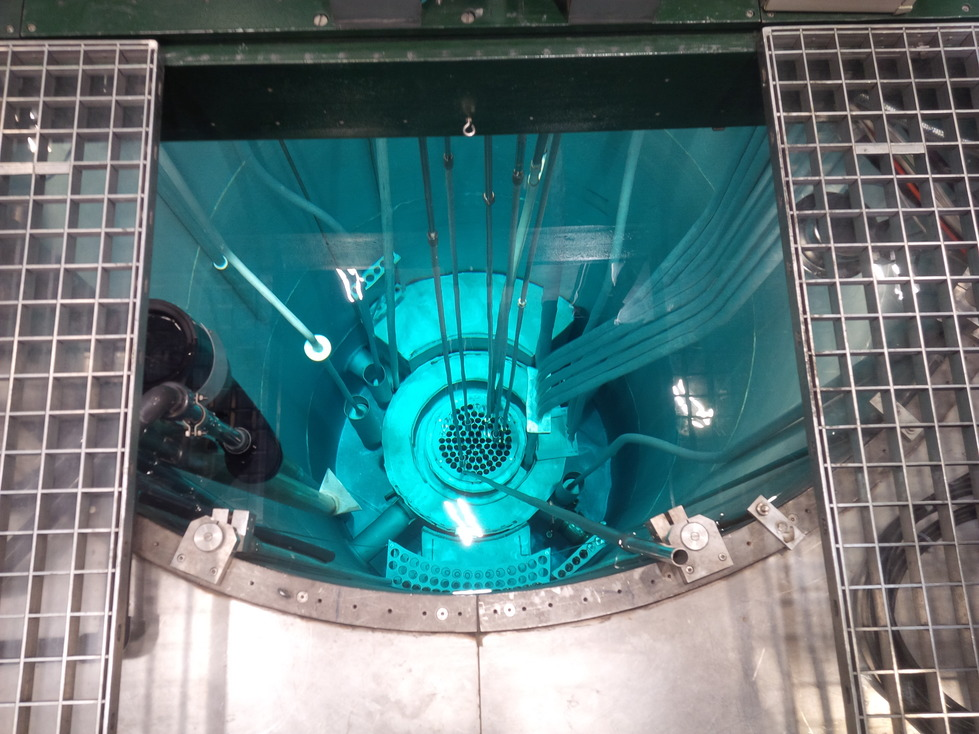
\includegraphics[scale=0.25]{../figuras/triga-thcoax-2.jpg}
  \\
  \vspace{0.2cm}
  \scriptsize{(Fonte: Thermocoax, França)}
\end{frame}

%\begin{frame}
%  \frametitle{O que é isso?}
%  \framesubtitle{Definições}
%  \begin{itemize}
%  \item \textbf{Neutrônica:} Estudo do transporte de nêutrons.
%    \begin{itemize}
%      \item \textbf{Seções de choque:} [Aguarde].
%      \end{itemize}
%  \item \textbf{Termo-hidráulica:} Estudo da transferência de calor e massa, processos fluido-mecânicos com transporte
%    de energia e massa em sistemas nucleares \cite{Todreas2012}.
%  \item \textbf{\textit{Software} Livre:} O usuário tem liberdade de executar, modificar e redistribuir versões, modificadas ou não,
%    de um programa \cite{Stallman2002}.
%%  \item \textbf{Memória compartilhada:} Forma padrão de utilização do mesmo espaço de memória pois dois ou mais programas de computador.
%  \item \textbf{Acoplamento (ou multi-física):} Análise de fenômenos físicos distintos de forma combinada \cite{Lethbridge2005}.
%  \end{itemize}
%  \centering
%  \alert{E por que acoplar?}
%  
%\end{frame}
%
%\subsection{Justificativa}
%-------------------------------------------------
%{\setbeamercolor{background canvas}{bg=black}
%  \setbeamercolor{frametitle}{fg=red}
%  \setbeamercolor{normal text}{fg=red}
\subsection{Justificativa}
  \begin{frame}
    \frametitle{Justificativa}
    \framesubtitle{Relações entre os fenômenos físicos}
    \centering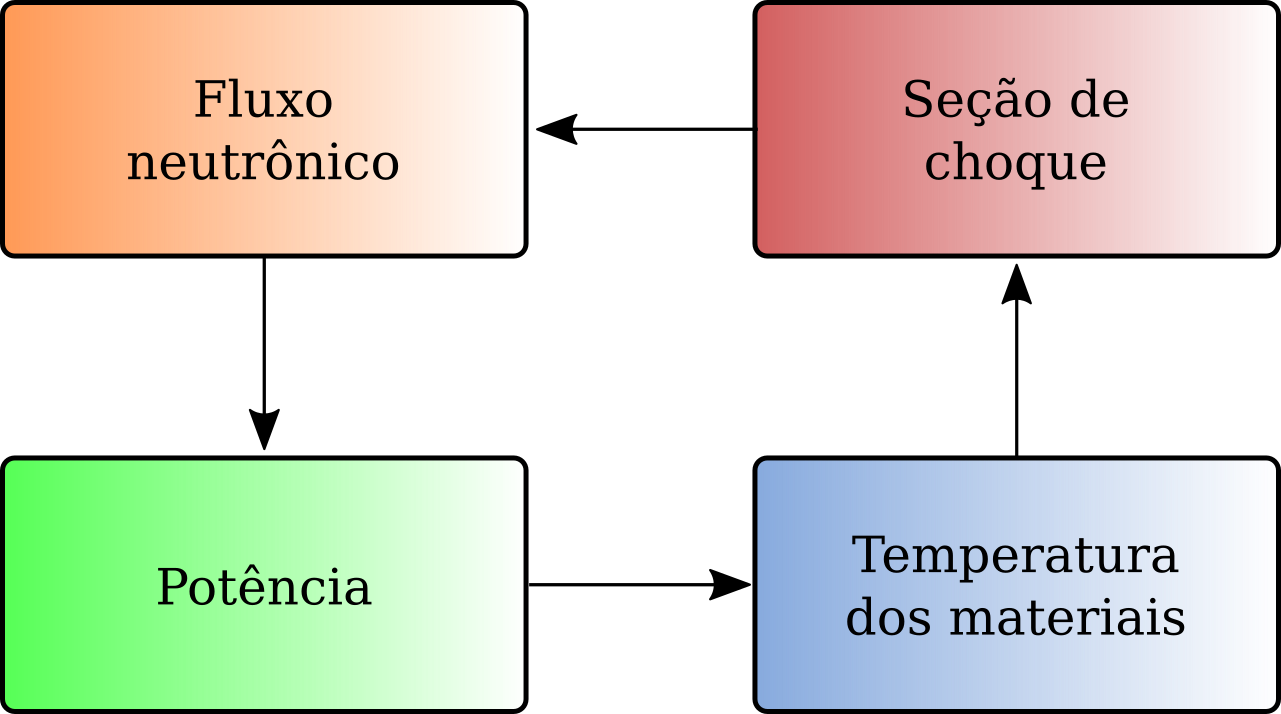
\includegraphics[scale=0.9]{../figuras/justificativa.png}
%    \centering\includegraphics[scale=0.9]{../figuras/justificativa-neg.png}
\end{frame}
%}

\subsection{Objetivo}
%-------------------------------------------------
\begin{frame}
  \frametitle{Objetivo}
%  \framesubtitle{Qual a razão de um sistema acoplado?}

\Large{Desenvolvimento de um sistema acoplado para cálculos neutrônicos e
  termo-hidráulicos aberto e gratuito basedo em \textit{CFD} e
  volumes finitos utilizando o mesmo domínio de solução.}
  
\end{frame}

\section{Metodologia}
%-------------------------------------------------
\begin{frame}
  \frametitle{Metodologia}
  \framesubtitle{Como acoplar neutrônica e termo-hidráulica?}
  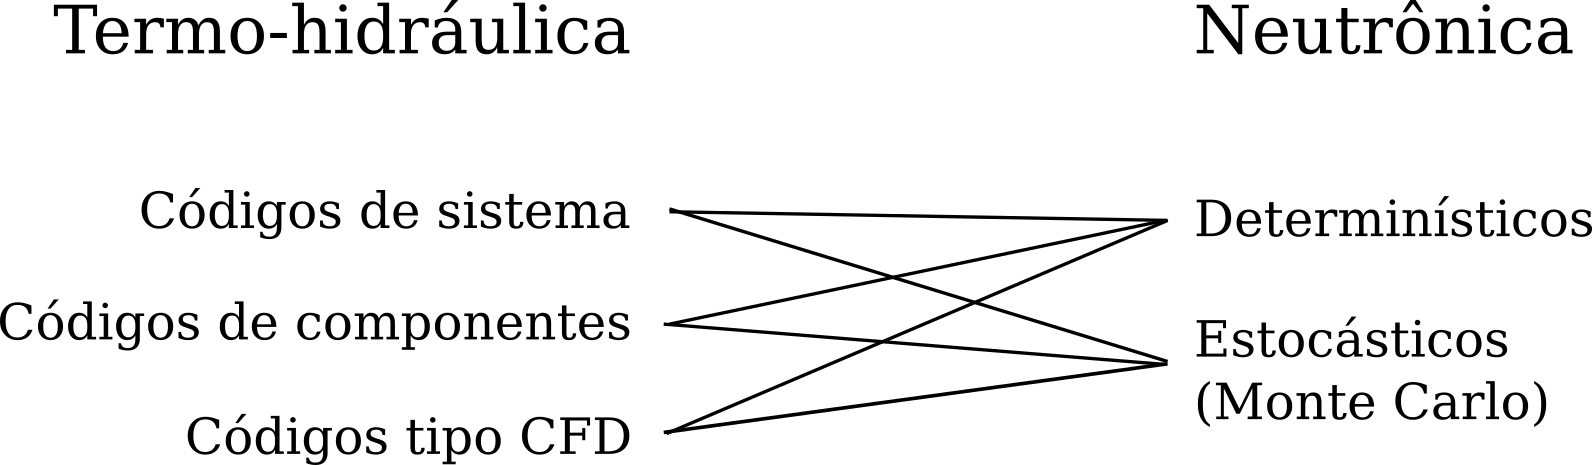
\includegraphics[scale=0.8]{../figuras/th-neu-1.png}
%  \begin{tikzpicture}
%    \node(img1) {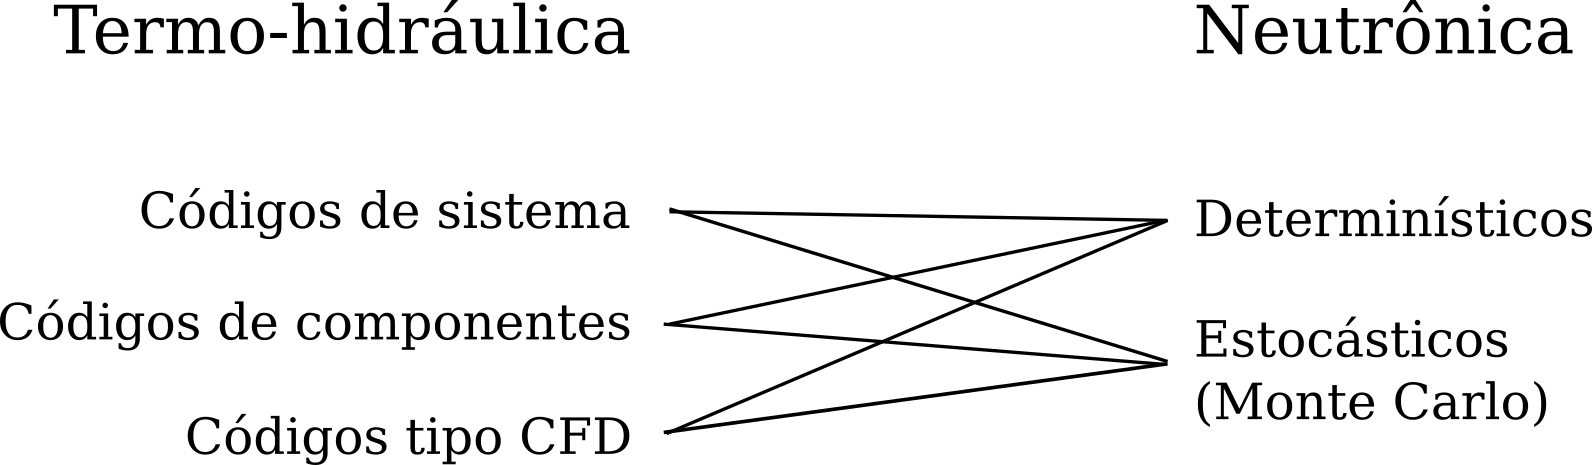
\includegraphics[scale=0.8]{../figuras/th-neu-1.png}};
%    \pause
%    \node(img2) {\includegraphics[scale=0.8]{../figuras/th-neu-2.png}};
%  \end{tikzpicture}
\end{frame}

%-------------------------------------------------
\begin{frame}[noframenumbering]
  \frametitle{Metodologia}
  \framesubtitle{Como acoplar neutrônica e termo-hidráulica?}
  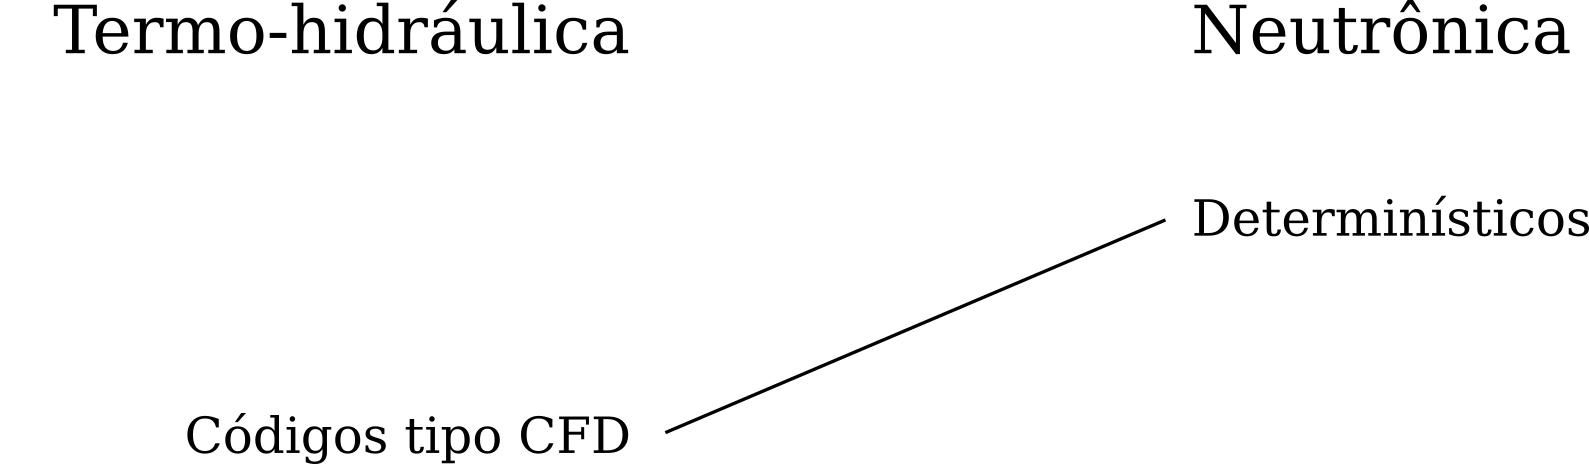
\includegraphics[scale=0.8]{../figuras/th-neu-4.png}
\end{frame}

%-------------------------------------------------
%{\setbeamercolor{background canvas}{bg=black}
%  \setbeamercolor{frametitle}{fg=red}
%  \setbeamercolor{framesubtitle}{fg=red}
%  \setbeamercolor{normal text}{fg=red}
%  \setbeamercolor{itemize item}{fg=white}
%\begin{frame}
%  \frametitle{Percurso}
%  \framesubtitle{O caminho é tortuoso...}
%  \textbf{Inicialmente:} \textit{Desenvolvimento do Acoplamento
%Neutrônico e Termo-hidráulico usando os códigos PARCS
%e OpenFOAM: Aplicação à Segurança de Reatores} \cite{PARCS2006}
%
%  \begin{itemize}
%    \item Trabalho \cite{Silva2013} e registro de \textit{software} \cite{TrigaFuel2013}.
%  \end{itemize}
%   \textbf{Doutorado sanduíche:} Universidade Politécnica de Valência.
%    Acoplamento com código da UPV, dessa vez aplicado a reatores
%    de potência (PWR).
%  \begin{itemize}
%    \item Trabalho \cite{Silva2015}.
%  \end{itemize}
%  \textbf{Finalmente:} \textit{Acoplamento neutrônico termo-hidráulico usando
%    os códigos milonga e OpenFOAM: uma abordagem com sotware livre}.
%  \begin{itemize}
%    \item Artigo (aceito).
%  \end{itemize}
%  \centering
%  \Large{Esta tese!}
%
%\end{frame}
%}
%  
%-------------------------------------------------
\begin{frame}
  \frametitle{Metodologia}
  \framesubtitle{Ferramentas usadas}
  CFD $\rightarrow$ \textit{Computational Fluid Dynamics}
  \\
  \vspace{0.5cm}
  É o estudo da Mecânica dos Fluidos e Transferência de Calor utilizando análise numérica.
  \\
  \vspace{0.5cm}
  Etapas comuns:
  \begin{itemize}
  \item Definição da geometria;
  \item \textbf{Discretização do domínio};
  \item Modelagem física;
  \item Definição de condições iniciais e condições de contorno;
  \item Solução propriamente dita;
  \item Pós-processamento;
  \end{itemize}
  \centering
  \vspace{0.5cm}
  \textit{Software} utilizado: \textit{OpenFOAM}
\end{frame}

%-------------------------------------------------
\begin{frame}
  \frametitle{Metodologia}
  \framesubtitle{Ferramentas usadas}
  Método Determinístico utilizado $\rightarrow$ Aproximação por difusão
  \\
  \vspace{0.5cm}
  Assume que os nêutrons se comportam como moléculas de um gás,
  se difundindo aleatoriamente de regiões de maior concentração
  para regiões de menor concentração.
  \\
  \vspace{0.5cm}
  É uma simplificação.
  \begin{itemize}
  \item Apesar disso, útil e aplicável em situações práticas
  \item Resolvida por métodos numéricos utilizando \textbf{discretização de domínio};
  \end{itemize}
\end{frame}

%-------------------------------------------------
{\setbeamercolor{background canvas}{bg=black}
  \setbeamercolor{frametitle}{fg=red}
  \setbeamercolor{normal text}{fg=red}
  \usebeamercolor[fg]{normal text}
  
\begin{frame}
  \frametitle{Discretização de domínio}
  \framesubtitle{O que é?}
\centering
Domínio contínuo e discretizado.
\\
\vspace{0.5cm}
  \centering
  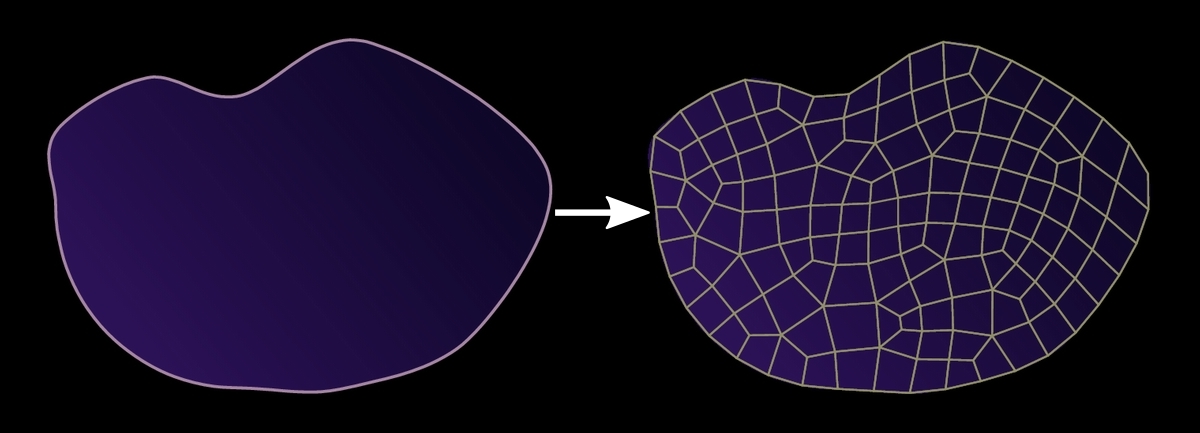
\includegraphics[scale=1.1]{../figuras/dom-neg.png}
  \vspace{0.5cm}
  \scriptsize(Fonte: Germán Theler)
\end{frame}
}
%-------------------------------------------------
\begin{frame}
  \frametitle{Metodologia}
  \framesubtitle{Equação de difusão discretizada}
  \textit{milonga} $\rightarrow$ Resolve a equação de difusão para nêutrons
  \\
  \vspace{0.5cm}
\begin{equation*}
  \label{eq:difusao}
  \begin{split}
  & 0 = \nabla . \big[\textcolor{blue}{-D_g({\mathbf{x}})} \nabla \phi_g(\mathbf{x})\big] 
- \textcolor{blue}{\Sigma_{tg}(\mathbf{x})}.\phi(\mathbf{x}) \\
& + \sum_{g'\neq g}^{G} \textcolor{blue}{\Sigma_{sg'\rightarrow g}(\mathbf{x})} . \phi_{g'}(\mathbf{x})
+ \chi(g)  \sum_{g'=1}^{G} \frac{\nu \textcolor{blue}{\Sigma_{fg'}(\mathbf{x})}}{k_{eff}} . \phi_{g'}(\mathbf{x}) \\
  \end{split}
  \end{equation*}
  
\end{frame}

%-------------------------------------------------
\begin{frame}
  \frametitle{Metodologia}
  \framesubtitle{Fenômenos físicos dependentes}
  %  Importante: falamos de reatores à água leve
  \centering
  \alert{Seções de choque}
  \\
  \vspace{0.5cm}
  O conceito de seção de choque é usado para descrever a probabilidade de cada
  tipo de reação nuclear.
  \\
  \vspace{0.5cm}
  Por hora, basta saber sobre as seções de choque que:
  \begin{itemize}
  \item são definidas para vários tipos de reações nucleares: fissão, espalhamento, absorção...
  \item dependem da velocidade (energia) dos nêutrons incidentes.
  \item dependem da densidade do alvo.
  \item \alert{não} são facilmente descritas em função da energia dos nêutrons.
  \end{itemize}
  
\end{frame}
%}

%-------------------------------------------------
{\setbeamercolor{background canvas}{bg=black}
  \setbeamercolor{frametitle}{fg=red}
  \setbeamercolor{normal text}{fg=red}

  \begin{frame}
  \frametitle{Seção de choque total para o $^{235}U$}
  \centering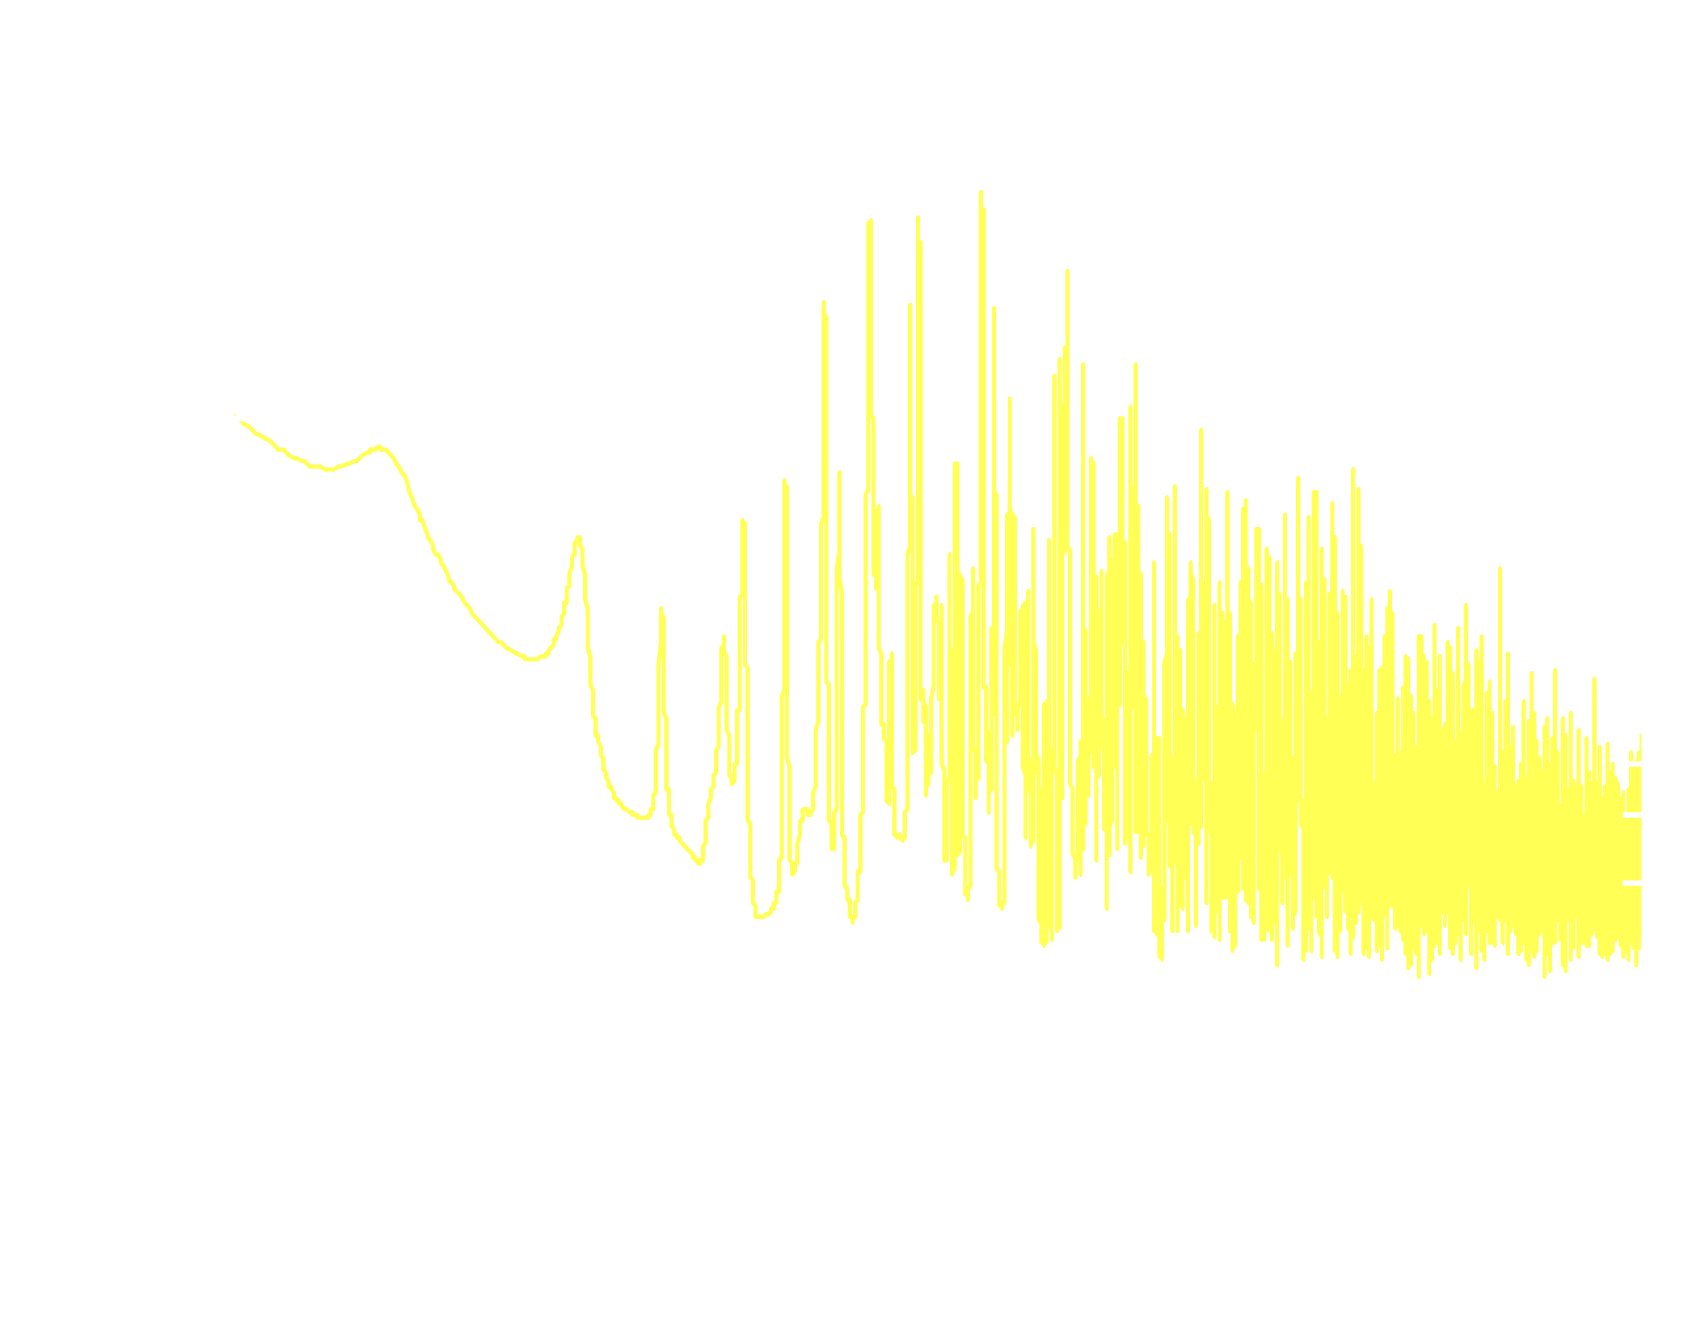
\includegraphics[scale=0.15]{../figuras/cu-neg.png}
  \\
  \centering
  \scriptsize{(Fonte: Projeto \textit{Multi-platform EXFOR-CINDA-ENDF}, V.Zerkin, IAEA-NDS, 1999-2016)}
\end{frame}
}

%-------------------------------------------------
\begin{frame}
  \frametitle{Metodologia}
  \framesubtitle{O acoplamento desenvolvido}
  %Equações da termo-hidráulica e da neutrônica $\rightarrow$ resolvidas por volumes finitos
  O sistema acoplado desenvolvido tem as seguintes características:
  \\
  \vspace{0.2cm}
  \begin{itemize}
  \item o domínio discretizado é representado por uma malha tridimensional;
  \item \textbf{a mesma malha é usada pelos dois códigos};
  \item \textbf{os dois códigos são livres $\rightarrow$ o sistema acoplado também};
  \item \textbf{trocam dados utilizando memória compartilhada};
  \end{itemize}
%  \centering
%  \vspace{0.5cm}
%  \Large{Objetivo: obtenção de detalhes no escoamento e na neutrônica}
  
\end{frame}

%-------------------------------------------------
{\setbeamercolor{background canvas}{bg=black}
  \setbeamercolor{frametitle}{fg=red}
  \usebeamercolor[fg]{normal text}
\begin{frame}
  \frametitle{Memória Compartilhada (\textit{Shared memory})}
  \framesubtitle{O que é?}
  \centering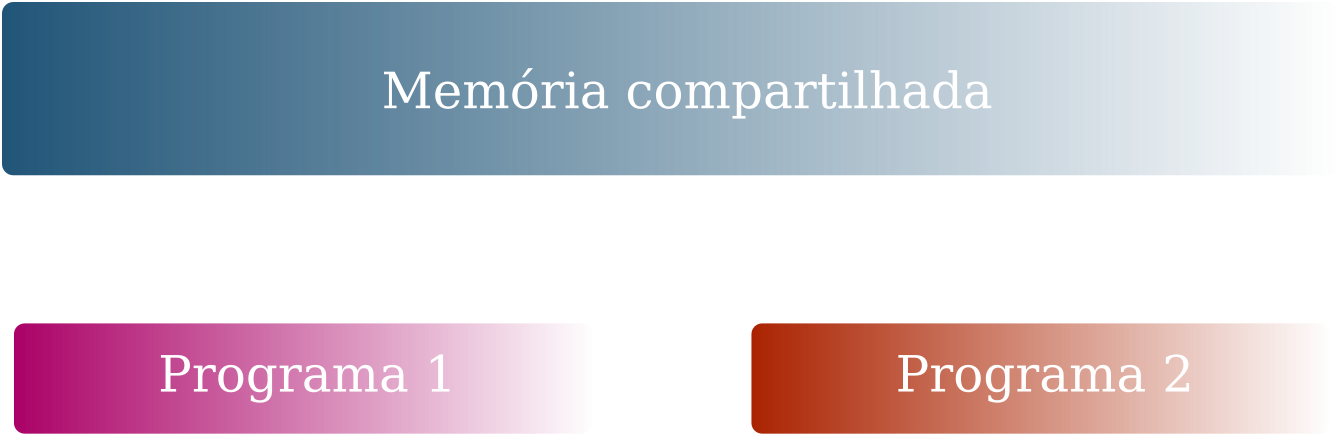
\includegraphics[scale=0.9]{../figuras/shm-neg.png}
\end{frame}
}

\subsection{Sistema acoplado}
%-------------------------------------------------
\begin{frame}
  \frametitle{O sistema acoplado}
  \framesubtitle{Visão Geral}
  \centering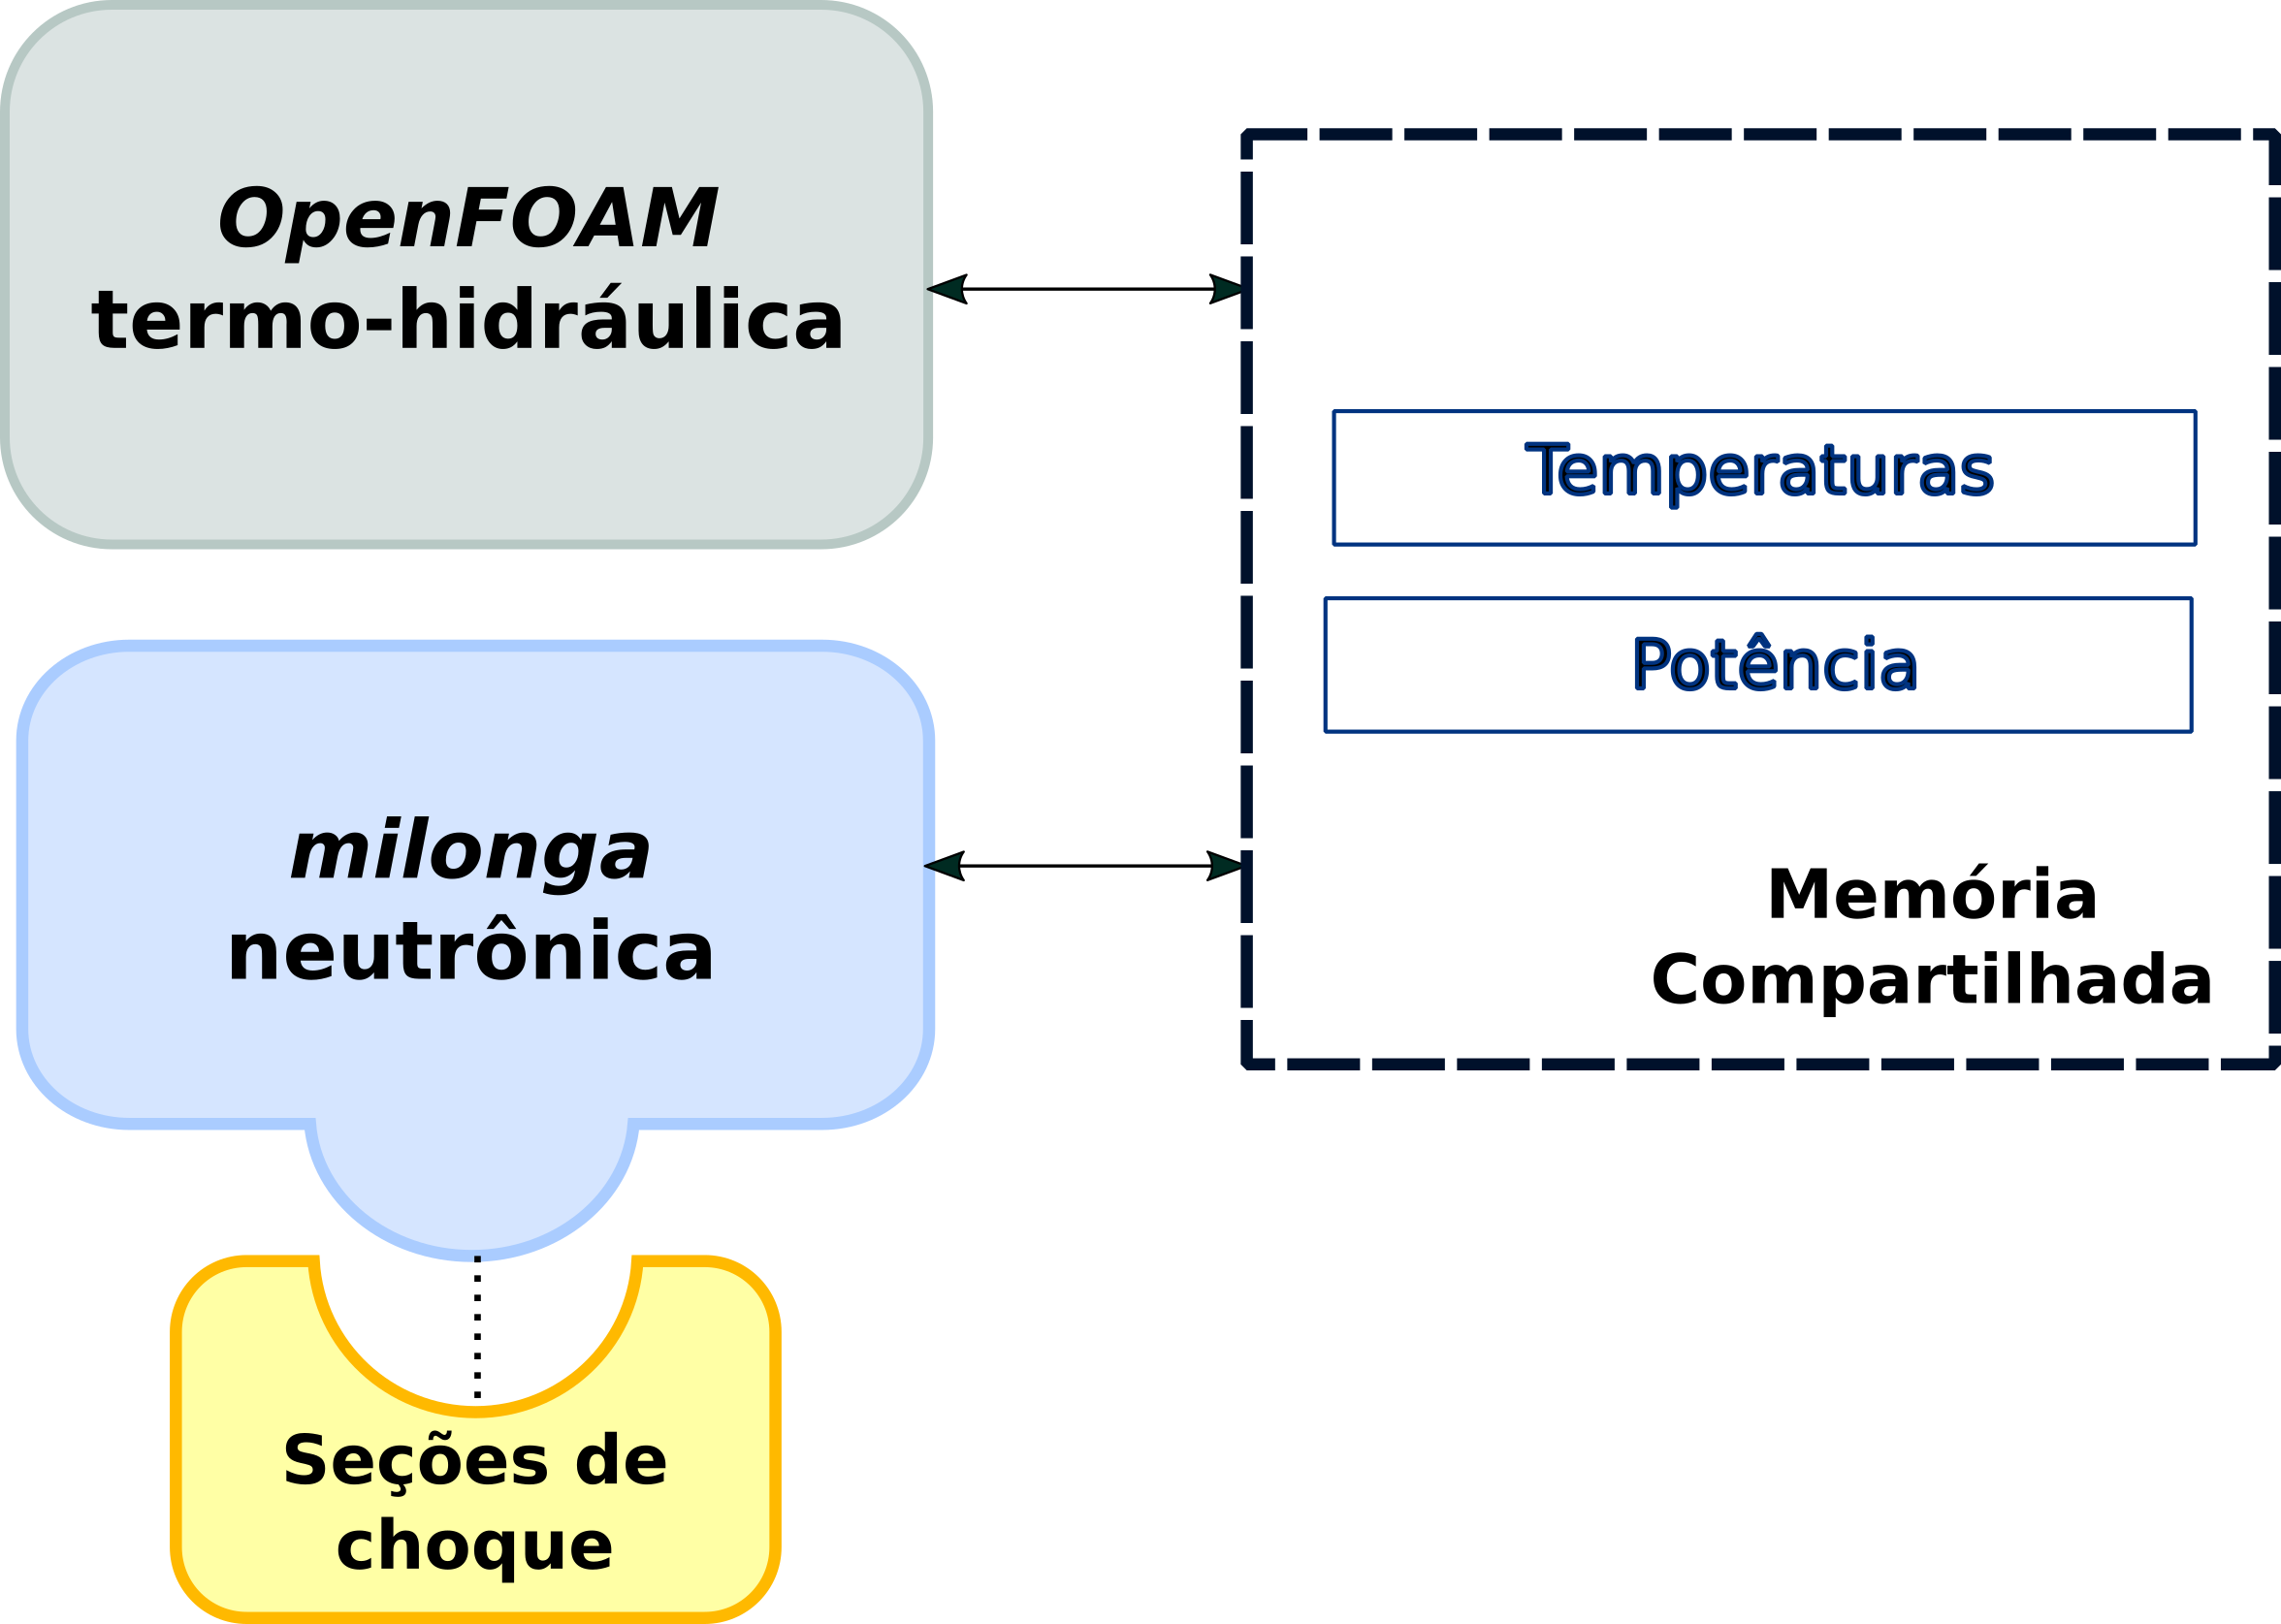
\includegraphics[scale=0.5]{../figuras/metodologia2.png}
\end{frame}


%-------------------------------------------------
%\begin{frame}
%  \frametitle{Metodologia}
%  \framesubtitle{Ferramentas usadas}
%  FVM $\rightarrow$ \textit{Finite Volume Method}
%  \\
%  \vspace{0.5cm}
%  Método para representar e calcular equações diferenciais parciais na forma
%  de equações algébricas.
%  \\
%  \vspace{0.5cm}
%  Como funciona?
%  \begin{itemize}
%  \item Valores são calculados em um \textbf{domínio discretizado};
%  \end{itemize}
%
%\end{frame}
%

\subsection{Implementação}
%-------------------------------------------------
\begin{frame}
  \frametitle{Desenvolvimento}
  \framesubtitle{Implementação}
  \centering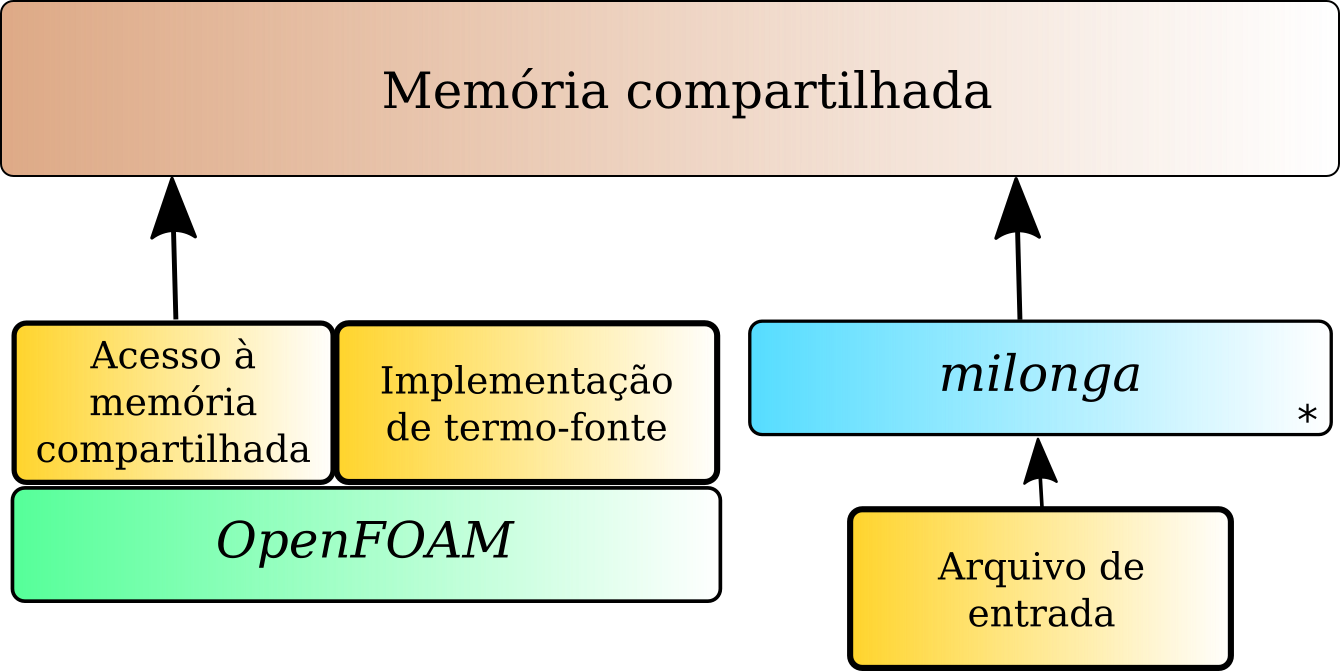
\includegraphics[scale=0.9]{../figuras/metod-2.png}
\end{frame}



%-------------------------------------------------
\begin{frame}[fragile]
  \frametitle{Acesso à memória compartilhada - Criação}
%  \framesubtitle{Exemplo1}
 \begin{lstlisting}%[caption={Fragmento do código-fonte da criação das estruturas de memória compartilhada.}\label{lst:createshm}]
   // Three C standard arrays are created to shared data with milonga
   double *shmTarray = NULL;
   double *shmQarray = NULL;
   
   void *shmT;
   void *shmQ;

   int shmTfile = 0;
   int shmQfile = 0;
   
   // Posix C semaphores
   sem_t *calcOf;
   sem_t *calcMil;
   
   // Posix structures initialization
   calcOf = sem_open("calcOf", O_CREAT, 0666);
   calcMil = sem_open("calcMil", O_CREAT, 0666);
   
   if(Pstream::master())
   {
     // Semaphores and shared memory files are tested at this point.
     // If milonga is not running, OpenFOAM runs uncoupled.
     shmTfile = shm_open("temperaturas", O_RDWR, 0666);
     shmQfile = shm_open("potencias", O_RDWR, 0666);
    
     if(shmTfile == -1 || shmQfile == -1) coupling = false; // Error finding shared memory
   }
 \end{lstlisting}
\end{frame}

%-------------------------------------------------
\begin{frame}[fragile]
  \frametitle{Acesso à memória compartilhada - Verificação}
 \begin{lstlisting}%[caption={Fragmento do código-fonte da criação das estruturas de memória compartilhada.}\label{lst:createshm}]
if(Pstream::master())
{
// After reading the shared memory files, they must be mapped to data
    shmT = mmap(NULL, totalNumberOfCells*sizeof(double), PROT_WRITE, MAP_SHARED, shmTfile, 0);
    shmQ = mmap(NULL, totalNumberOfCells*sizeof(double), PROT_WRITE, MAP_SHARED, shmQfile, 0);

// Check if all files were properly mapped
if((shmT == MAP_FAILED || shmQ == MAP_FAILED) && (coupling)) exit(errno); // Error mapping shared memory

// Make a C++ cast
    shmTarray = reinterpret_cast<double*>(shmT);
    shmQarray = reinterpret_cast<double*>(shmQ);
}
 \end{lstlisting}
\end{frame}

%-------------------------------------------------
\begin{frame}[fragile]
  \frametitle{Criação/Leitura do campo volumétrico de potências}
 \begin{lstlisting}
  PtrList<volScalarField> qVol(solidRegions.size());

  // Read Q if it exists. If not, create a null (zero) volScalarField
  IOobject Qfile("Q", runTime.timeName(), solidRegions[i],
                 IOobject::READ_IF_PRESENT, IOobject::AUTO_WRITE);

  // Must check it before creating the field
  if(Qfile.headerOk())
  {
    // Create a qvol field from dictionary
    qVol.set(i, new volScalarField (Qfile, solidRegions[i]));
  }
  else
  {
    // If file is not there, create a new IOobject
    // setting the dimensions of the field
    qVol.set(i,
    new volScalarField(IOobject
        ("Q", runTime.path(), solidRegions[i], IOobject::NO_READ,
          IOobject::AUTO_WRITE), solidRegions[i], dimensionedScalar
            ("dimension", dimensionSet(1, -1, -3, 0, 0), scalar(0.0))
        )
    );
  }
 \end{lstlisting}
\end{frame}

%-------------------------------------------------
\begin{frame}[fragile]
  \frametitle{Adição do termo-fonte à equação de energia do sólido}
 \begin{lstlisting}
  {
    for (int nonOrth=0; nonOrth<=nNonOrthCorr; nonOrth++)
    {
      fvScalarMatrix hEqn
      (
      - fvm::laplacian(betav*alpha, h, "laplacian(alpha,h)")

      // Source-term added to the equation
      - Q
      );

      hEqn.relax();
      hEqn.solve();
    }
  }
 \end{lstlisting}
\end{frame}


\subsection{Algoritmos}
%-------------------------------------------------
\begin{frame}
  \frametitle{Algoritmos}
  \framesubtitle{Controle da comunicação entre os códigos.}
  A memória é compartilhada $\rightarrow$ quem acessa quando?  
  \\
  \vspace{0.5cm}
  São usados semáforos:
  \begin{itemize}
  \item Evitam a ocorrência de condição de corrida;
  \item Mantém a atomicidade das operações;
  \item Garantem a não corrupção dos dados;
  \end{itemize}
  \vspace{0.5cm}
  O controle da comunicação é diferente para a neutrônica e termo-hidráulica.
\end{frame}


%-------------------------------------------------
\begin{frame}
  \frametitle{Algoritmo de controle da comunicação}
  \framesubtitle{Termo-hidráulica}
  \centering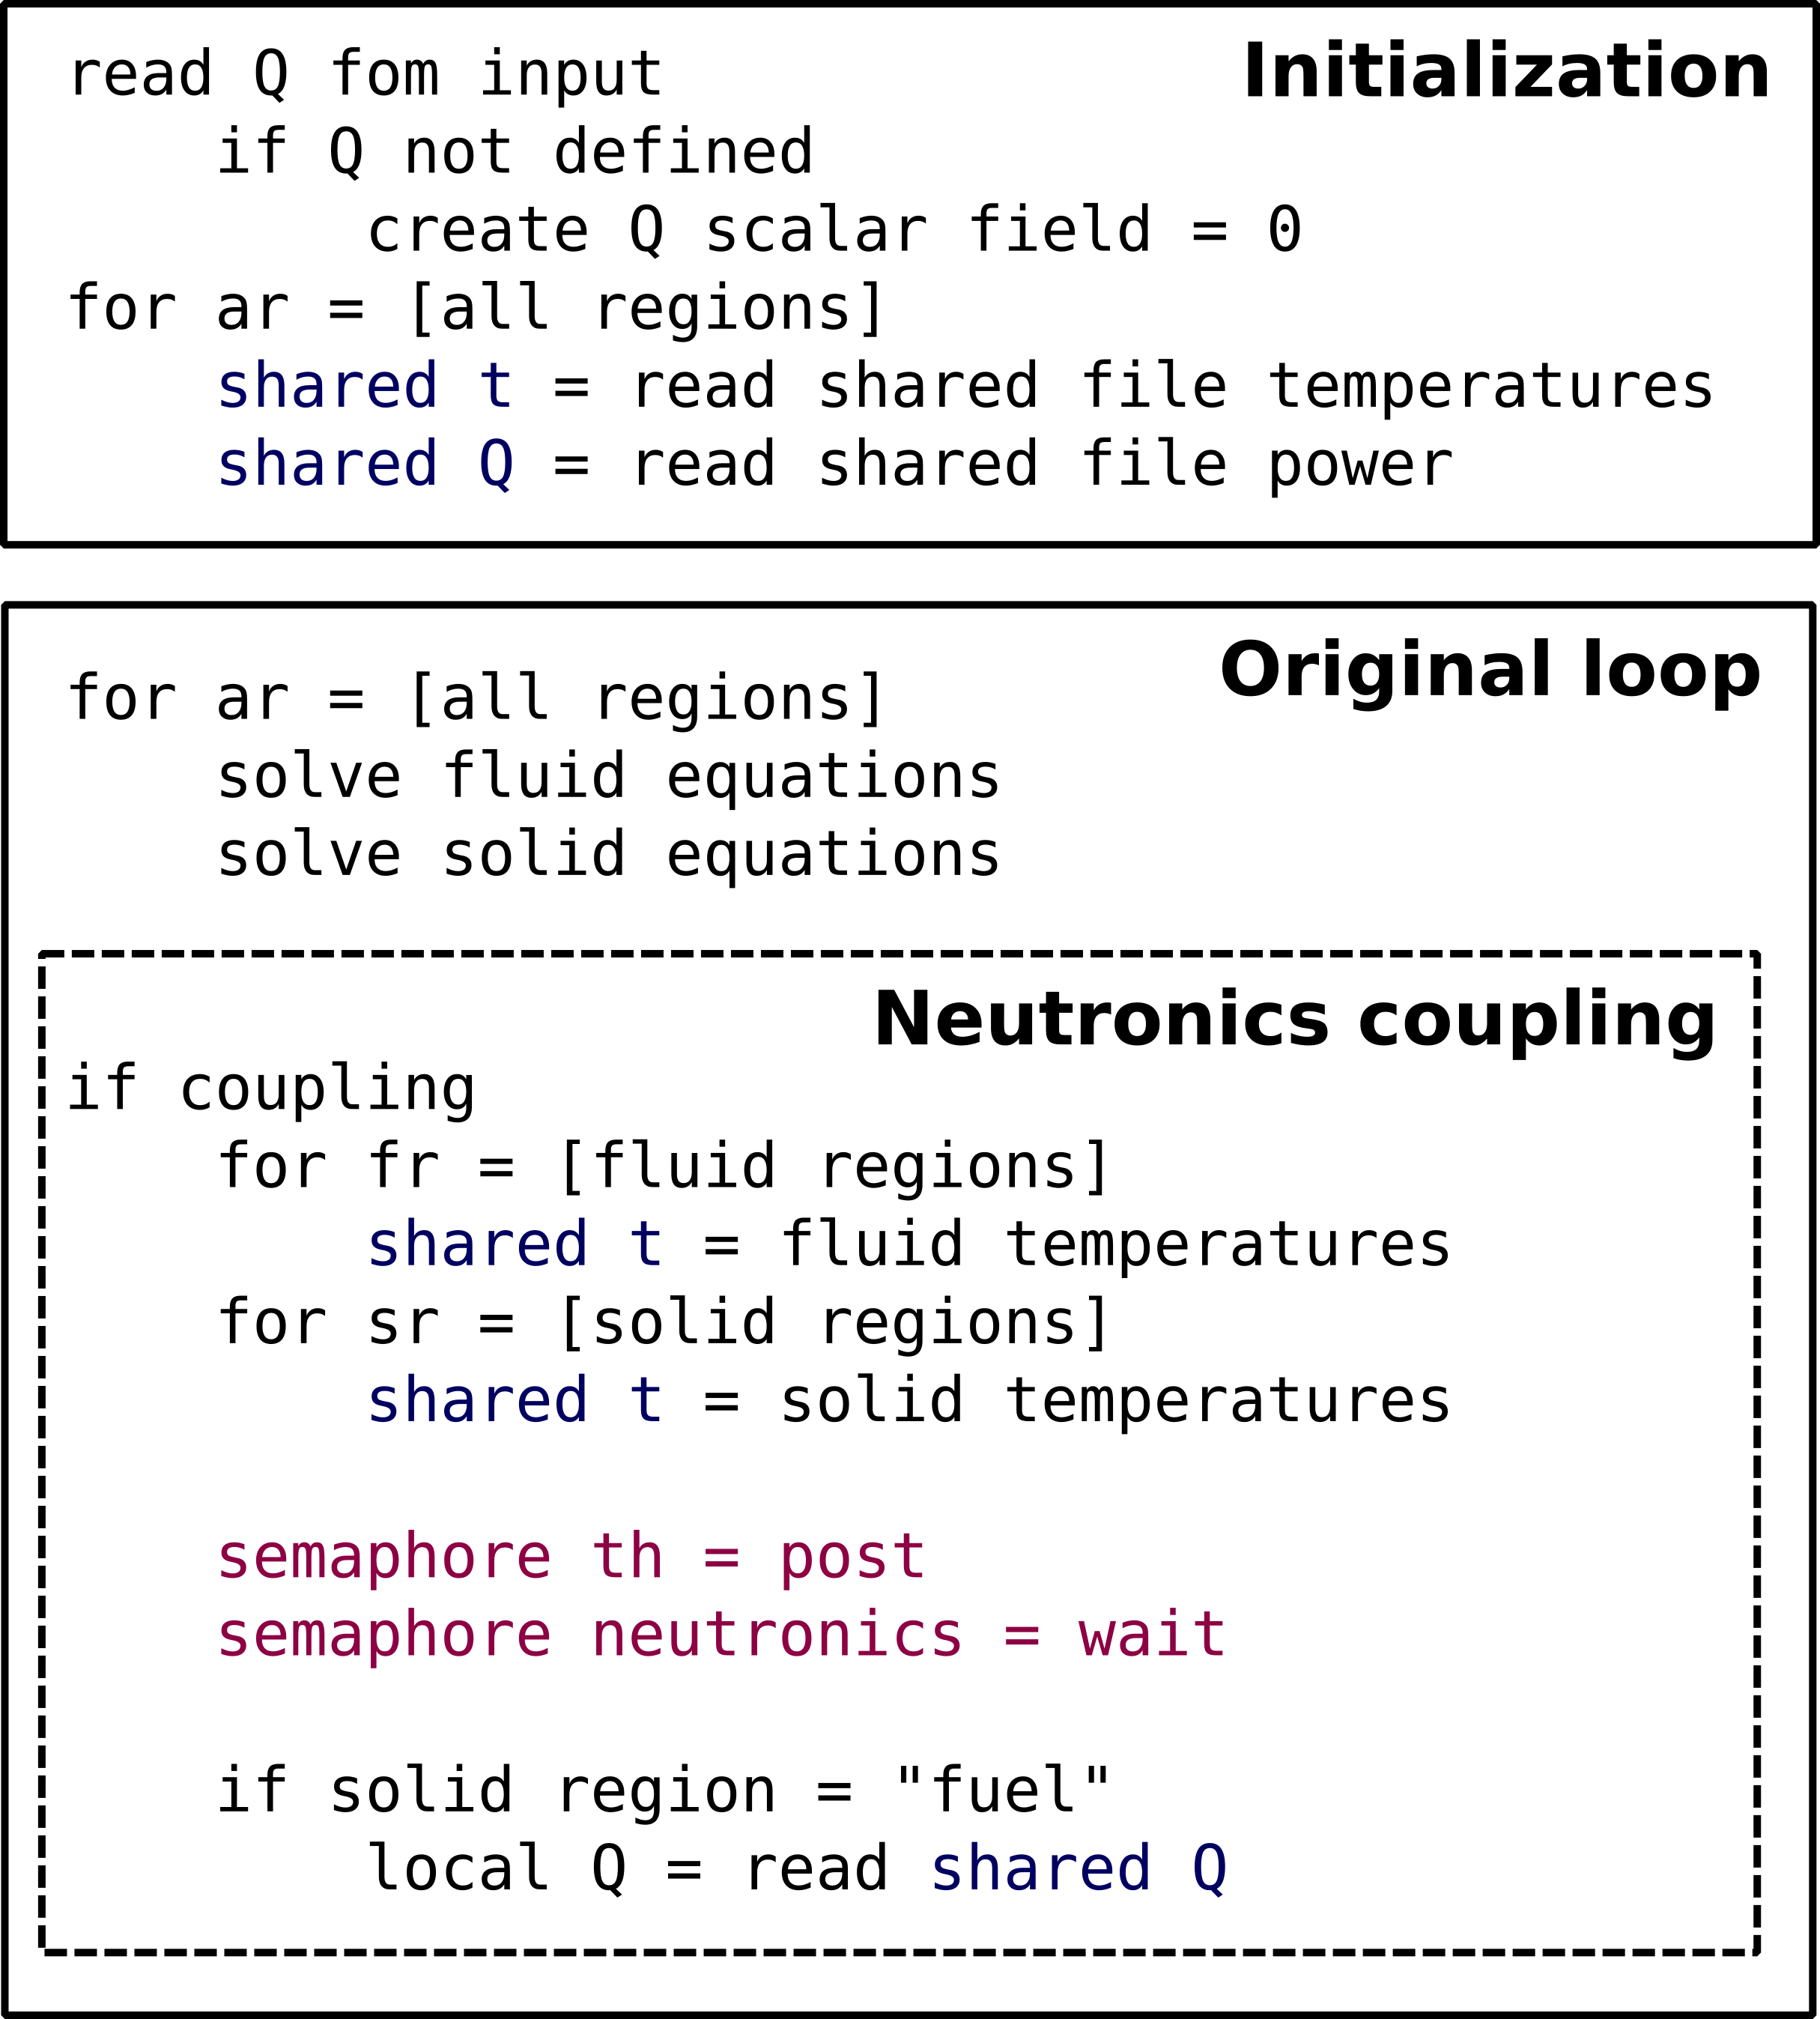
\includegraphics[scale=0.3]{../figuras/algoritmo_openfoam.png}  
\end{frame}


%-------------------------------------------------
\begin{frame}
  \frametitle{Algoritmo de controle de comunicação}
  \framesubtitle{Neutrônica}
  \centering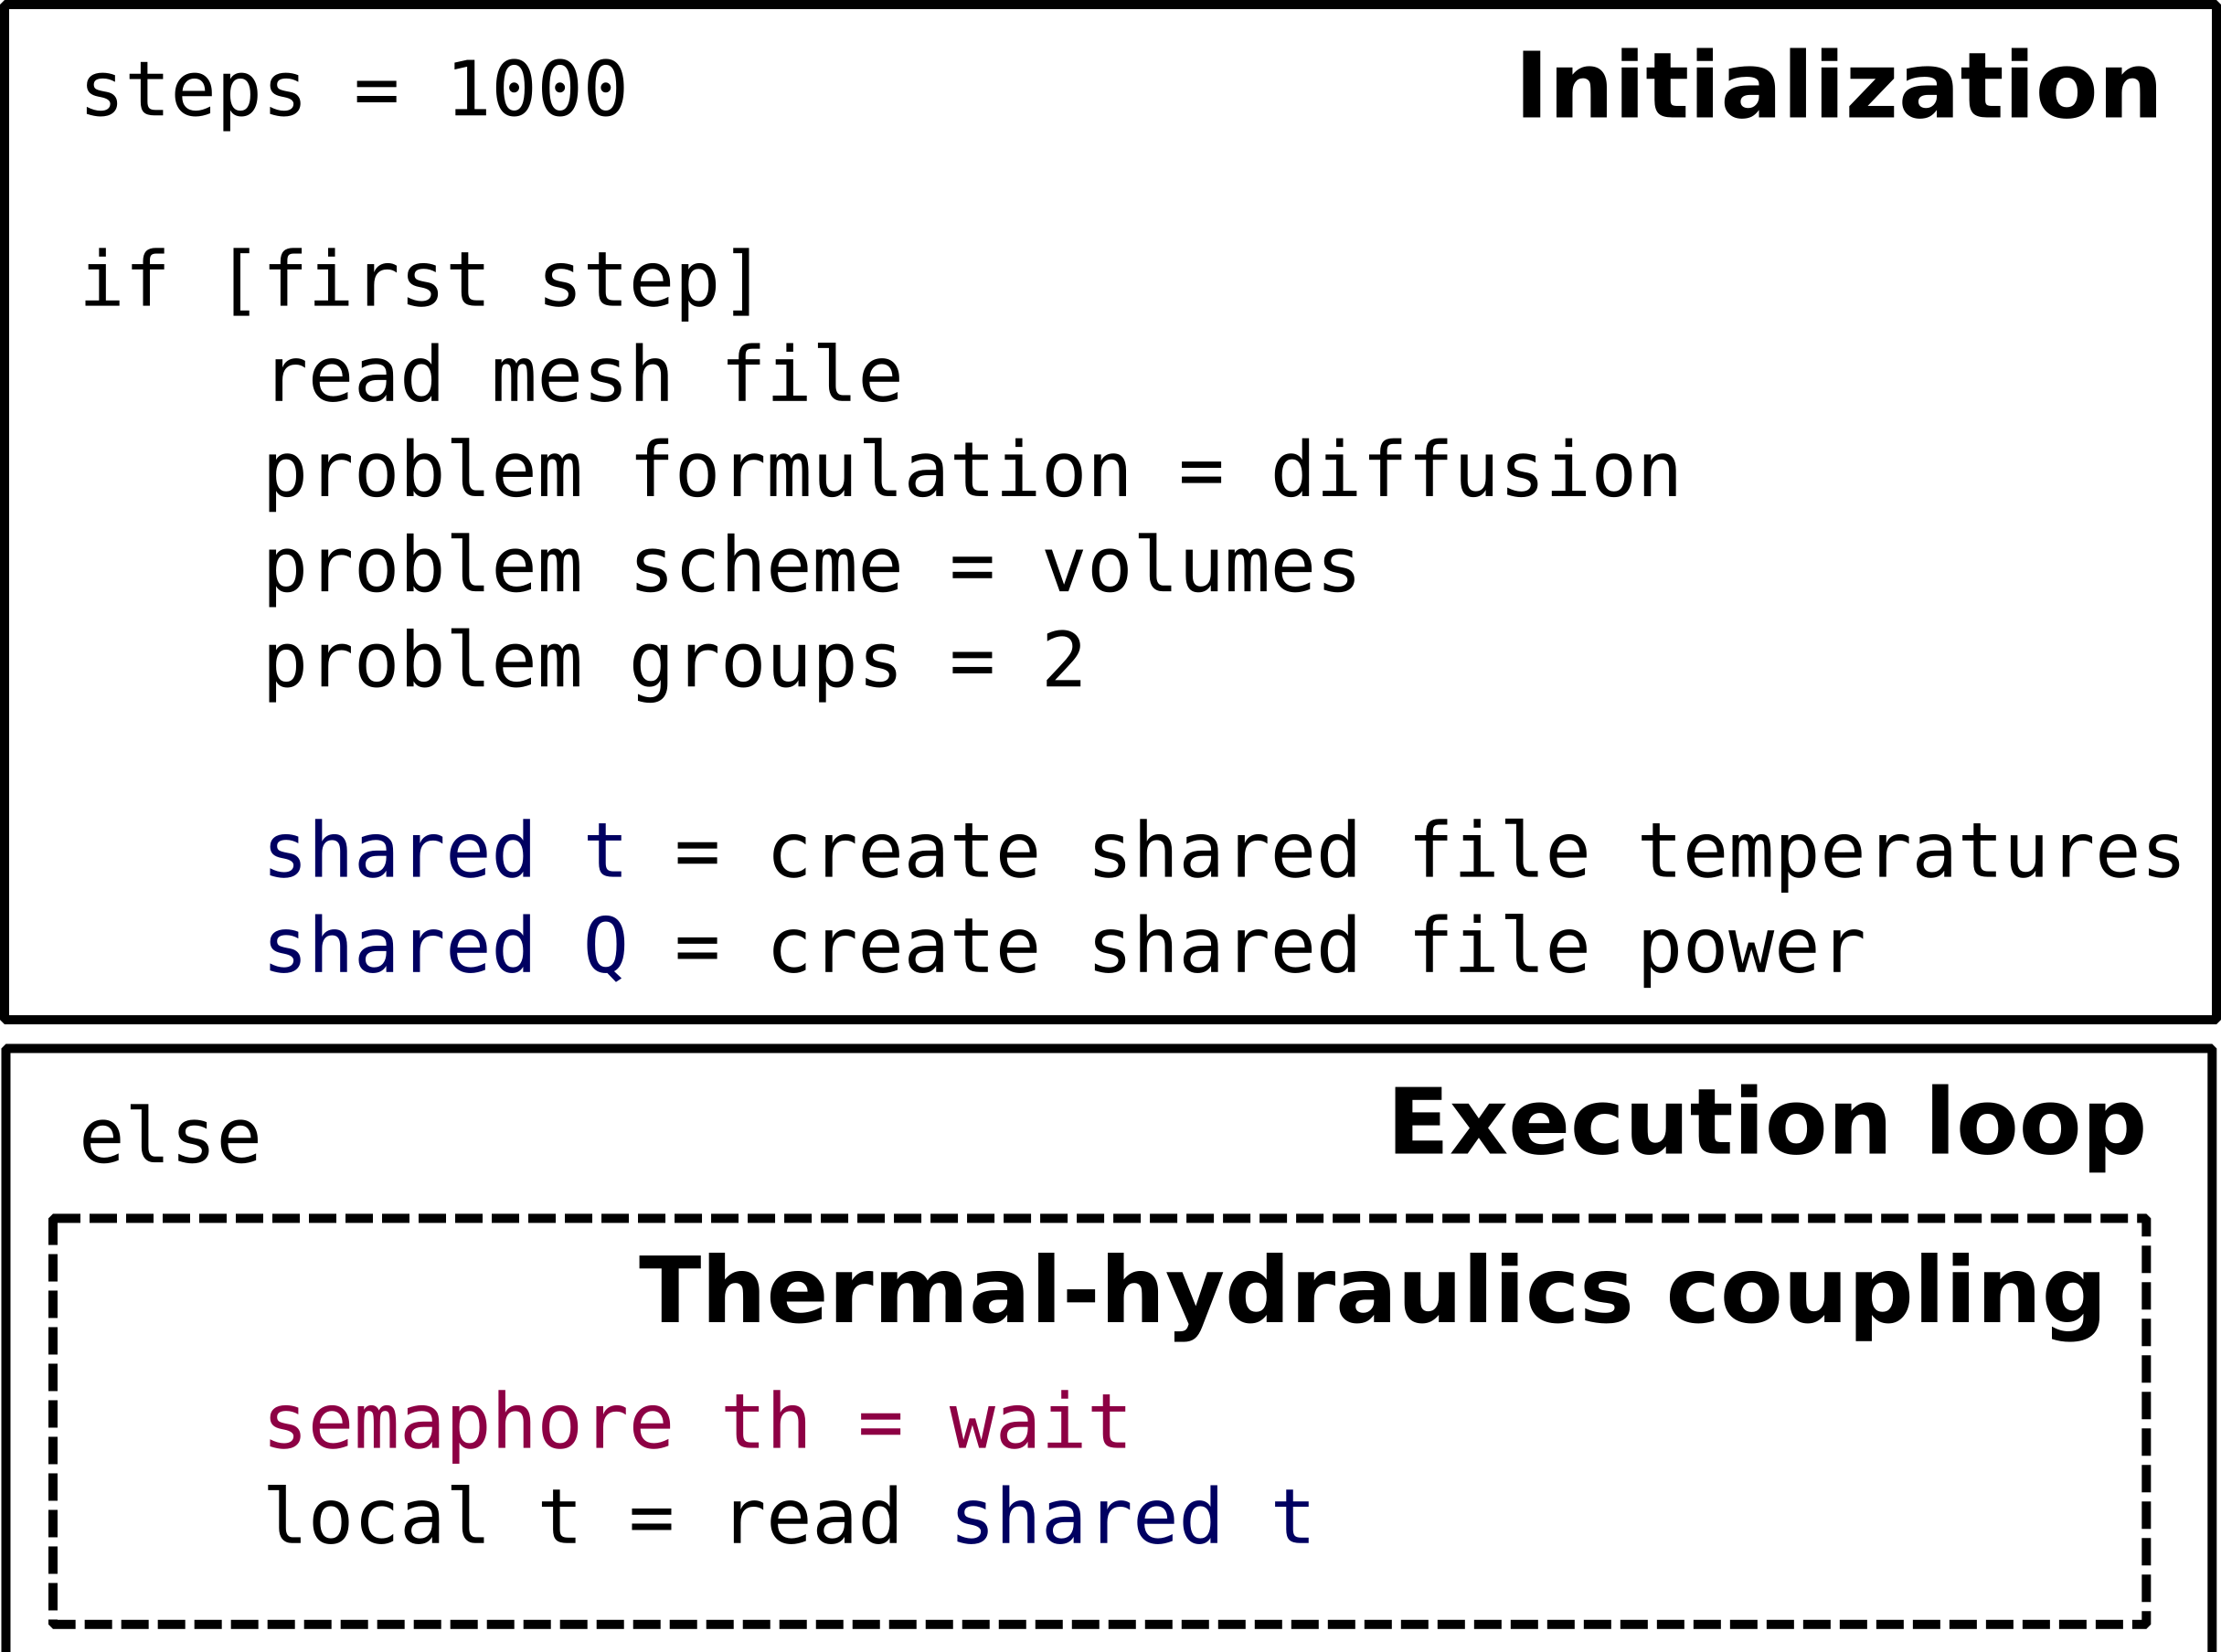
\includegraphics[scale=0.4]{../figuras/algo-mil-apre1.png}
\end{frame}

%-------------------------------------------------
\begin{frame}
  \frametitle{Algoritmo de controle de comunicação}
  \framesubtitle{Neutrônica}
  \centering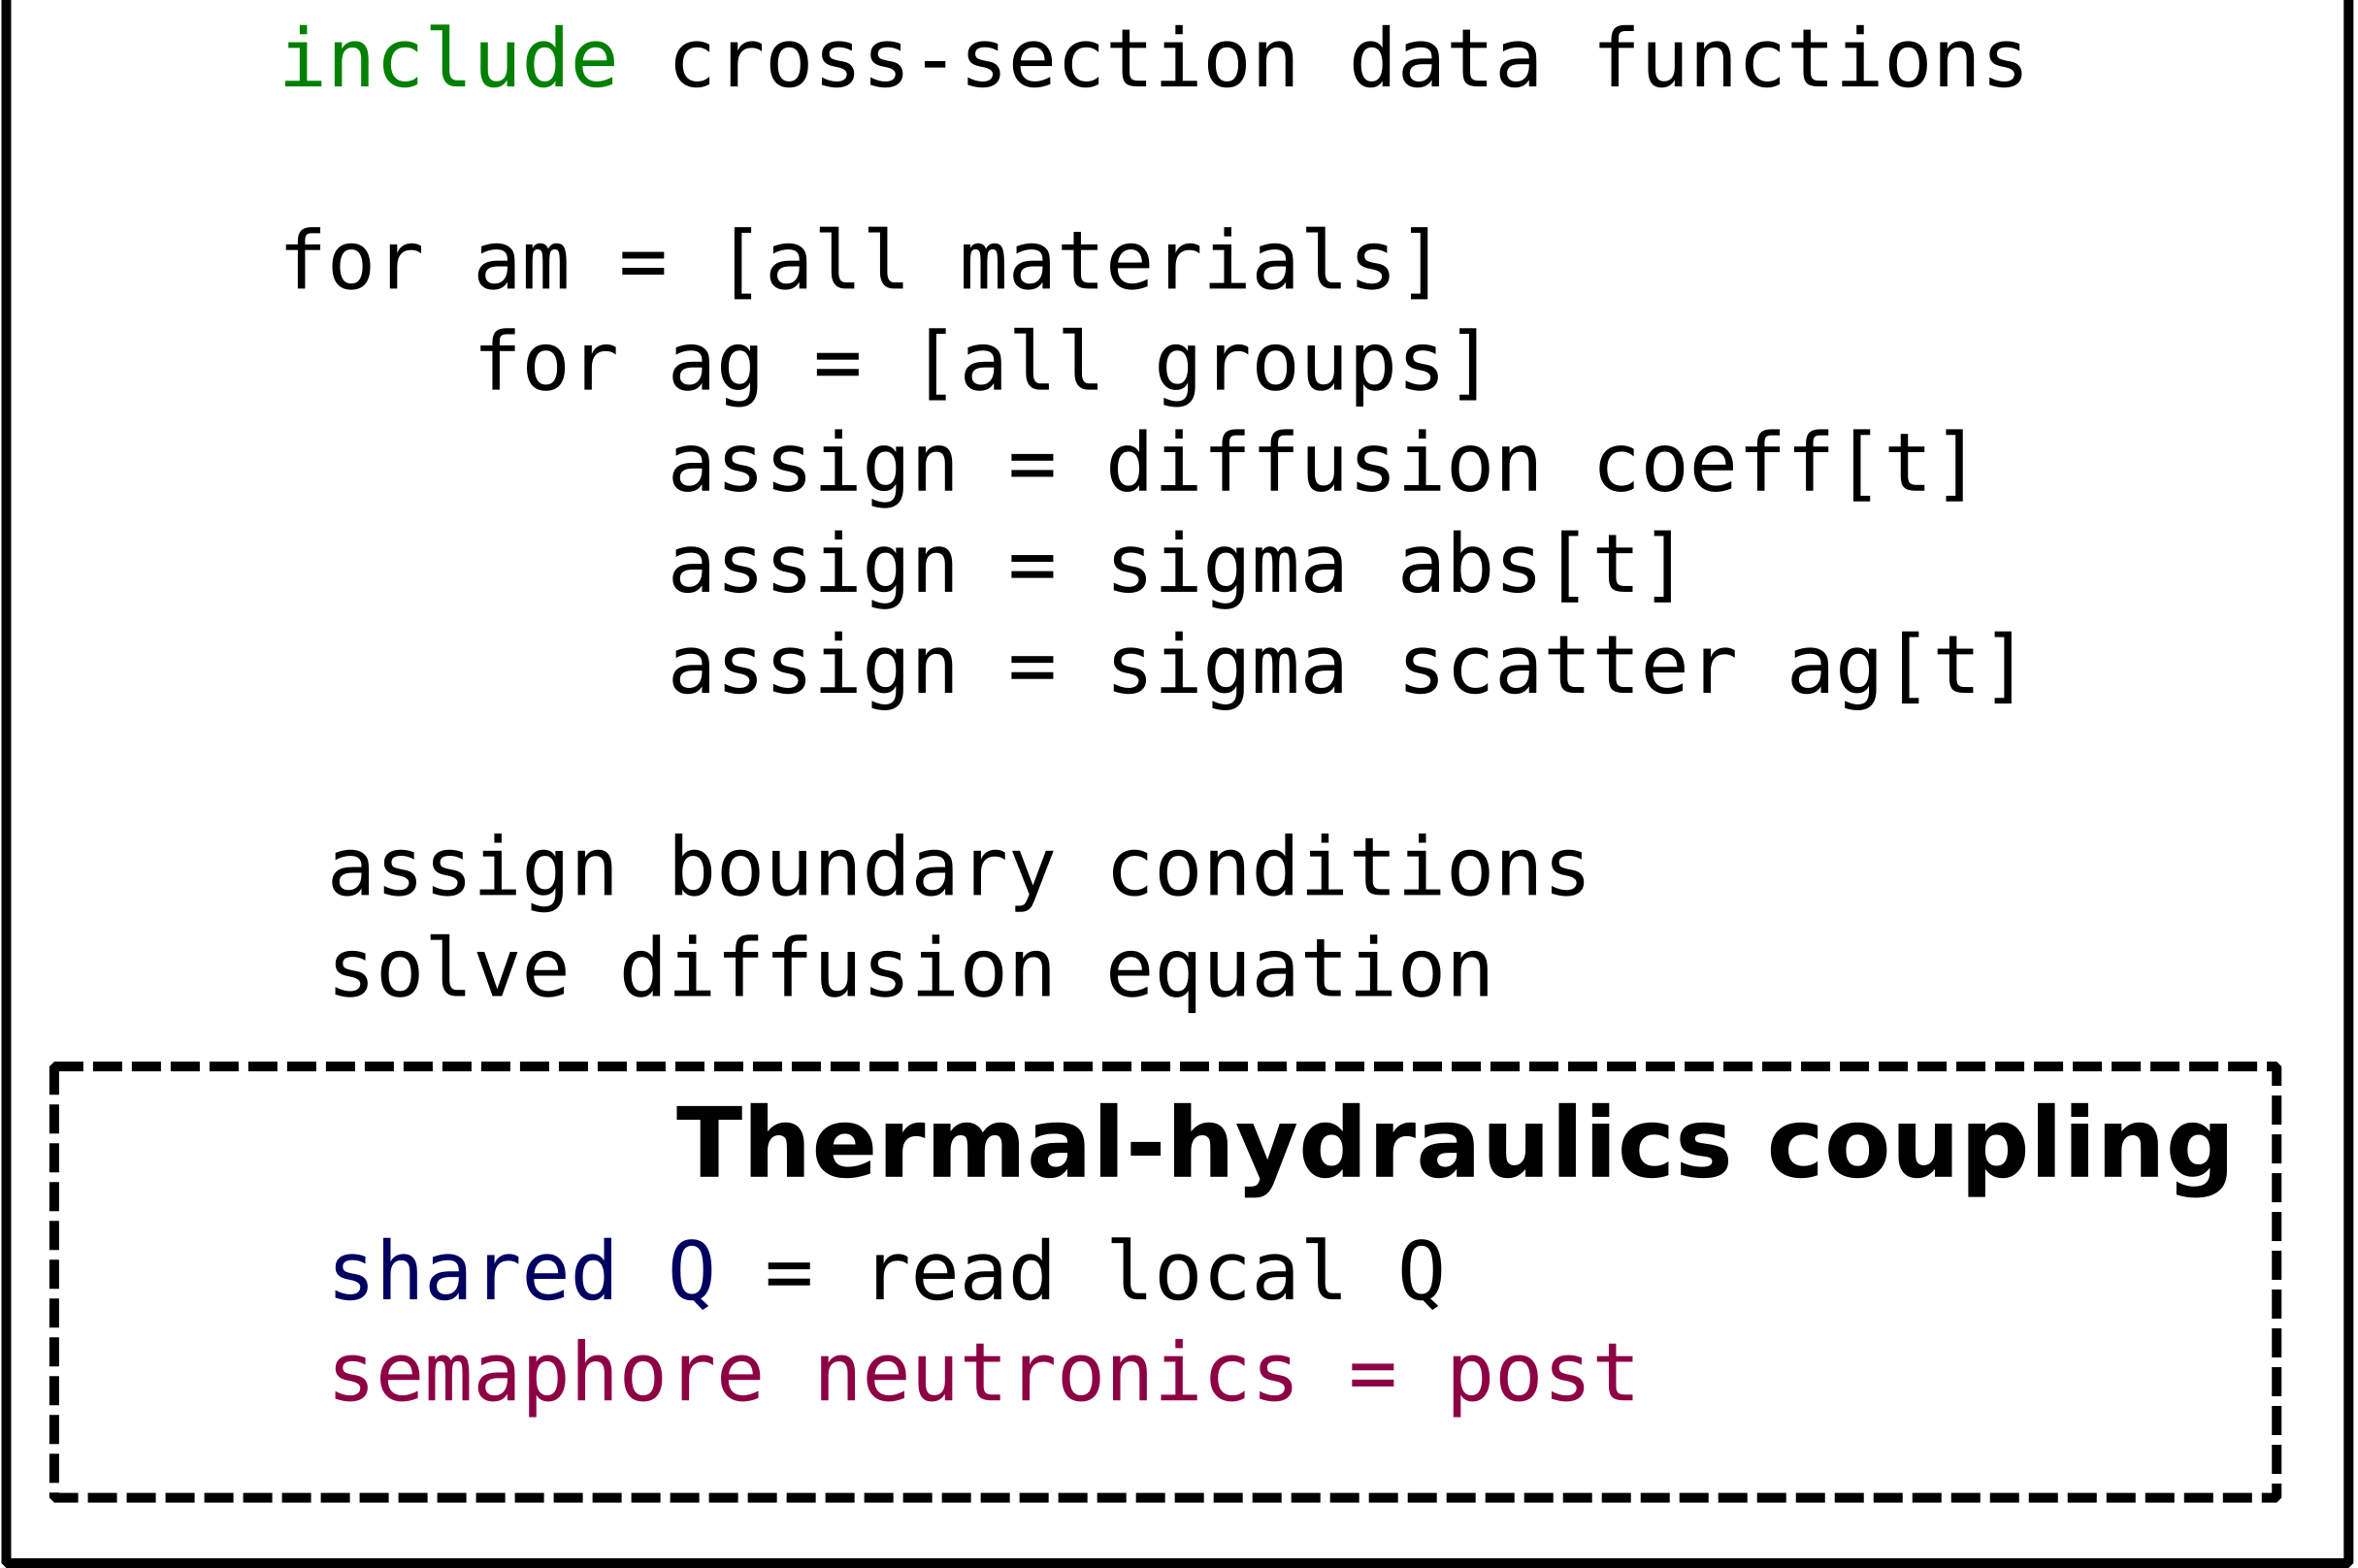
\includegraphics[scale=0.4]{../figuras/algo-mil-apre2.png}
\end{frame}

\subsection{Atualização das seções de choque}
%-------------------------------------------------
\begin{frame}
  \frametitle{Atualização das seções de choque}
  \framesubtitle{Antes de atualizar, é preciso \textbf{gerá-las}}
  Seções de choques para 2 grupos de nêutrons.\\
  \vspace{0.2cm}
  Utilização de uma metodologia estabelecida \cite{Reis2015}.\\
  \vspace{0.2cm}
  Utilização de um código específico: WIMSD-5B (\alert{restrito}).\\
  \vspace{0.2cm}
  \begin{itemize}
  \item modelo de célula mantendo a razão $\frac{material\quad físsil}{moderador}$;
  \item seções de choque geradas para 4 conjuntos de temperaturas;
  \item cada conjunto com as temperaturas dos 3 materiais;
  \end{itemize}
  \centering
  \vspace{0.2cm}
  \begin{tabular}{lrrrr}
    \multicolumn{5}{c}{Temperaturas dos materiais}                                                                                                       \\ \hline
    & \multicolumn{1}{l}{$T_1${[}K{]}} & \multicolumn{1}{l}{$T_2${[}K{]}} & \multicolumn{1}{l}{$T_3${[}K{]}} & \multicolumn{1}{l}{$T_4${[}K{]}}      \\ \hline
    Combustível  & 300                             & 400                             & 500                             & 600                             \\ \hline
    Revestimento & 300                             & 396                             & 403                             & 410                             \\ \hline
    Refrigerante & 300                             & 308,5                           & 317                             & 341                            
  \end{tabular}

\end{frame}

%-------------------------------------------------
\begin{frame}
  \frametitle{Atualização das seções de choque}
  \framesubtitle{Uma vez geradas, são apenas \textit{atualizadas}}
  A atualização é feita por interpolação linear simples.
  \\
  \vspace{0.2cm}
  Supondo que a temperatura em um material qualquer é de $350K$:
  \\
  \vspace{0.2cm}
  \texttt{assign = sigma abs[t]} é na prática:
  \centering
  \\
  \vspace{0.2cm}
  \begin{tabular}{llll}
                 & T=300  & \textcolor{red}{T=350} & T=400 \\ \hline
    $\Sigma_{A1}(T)$ & 0,771135       & \textcolor{red}{0,777381}         & 0,783626      
  \end{tabular}
  \\
  \vspace{0.2cm}
  Tem-se então:
  \\
  \vspace{0.2cm}
  $\Sigma_{A1}(350)$ = 0,777381.
  \\
  \vspace{0.2cm}
  Isso é feito para \textbf{cada} coeficiente de \textbf{cada} material para \textbf{cada} célula.
\end{frame}



%-------------------------------------------------
{\setbeamercolor{background canvas}{bg=black}
  \setbeamercolor{frametitle}{fg=red}
  \setbeamercolor{normal text}{fg=red}
  \usebeamercolor[fg]{normal text}

\begin{frame}
  \frametitle{O que significa o asterisco?}
  \framesubtitle{Mais um pouco de \textit{software} livre}
  \centering
  
\includegraphics[scale=1.0]{../figuras/mil-asterisco-neg.png}
  $\rightarrow$ correção no \textit{milonga}
  \\
  \vspace{0.5cm}
  Correção (\textit{patch}) submetida diretamente ao autor.
  \\
  Correção incorporada ao código.
  \\
  \vspace{0.5cm}
  \Large{$\rightarrow$ Contribuição para a comunidade.}
\end{frame}
}



\section{Aplicação}
%-------------------------------------------------
\begin{frame}
  \frametitle{Aplicação}
  \framesubtitle{Modelo \textbf{simplificado} de combustível do reator TRIGA IPR-R1}
  \vspace{0.2cm}
  \raggedright
%  \\
  Um modelo simplificado é útil para verificar o funcionamento do sistema desenvolvido.
  \\
  \vspace{0.2cm}
  \textbf{Prova de conceito}: do inglês ``proof of concept''.
  \\
  \vspace{0.2cm}
  Definição do dicionário \textit{Oxford:[mass noun] Evidence, typically deriving from an experiment or pilot project, which demonstrates that a design concept, business proposal, etc. is feasible: ``In academia, he says, a narrowly focused solution is acceptable as a proof of concept.''}
\end{frame}

%-------------------------------------------------
\begin{frame}
  \frametitle{Aplicação}
  \framesubtitle{Modelo \textbf{simplificado} de combustível do reator TRIGA IPR-R1}
  \centering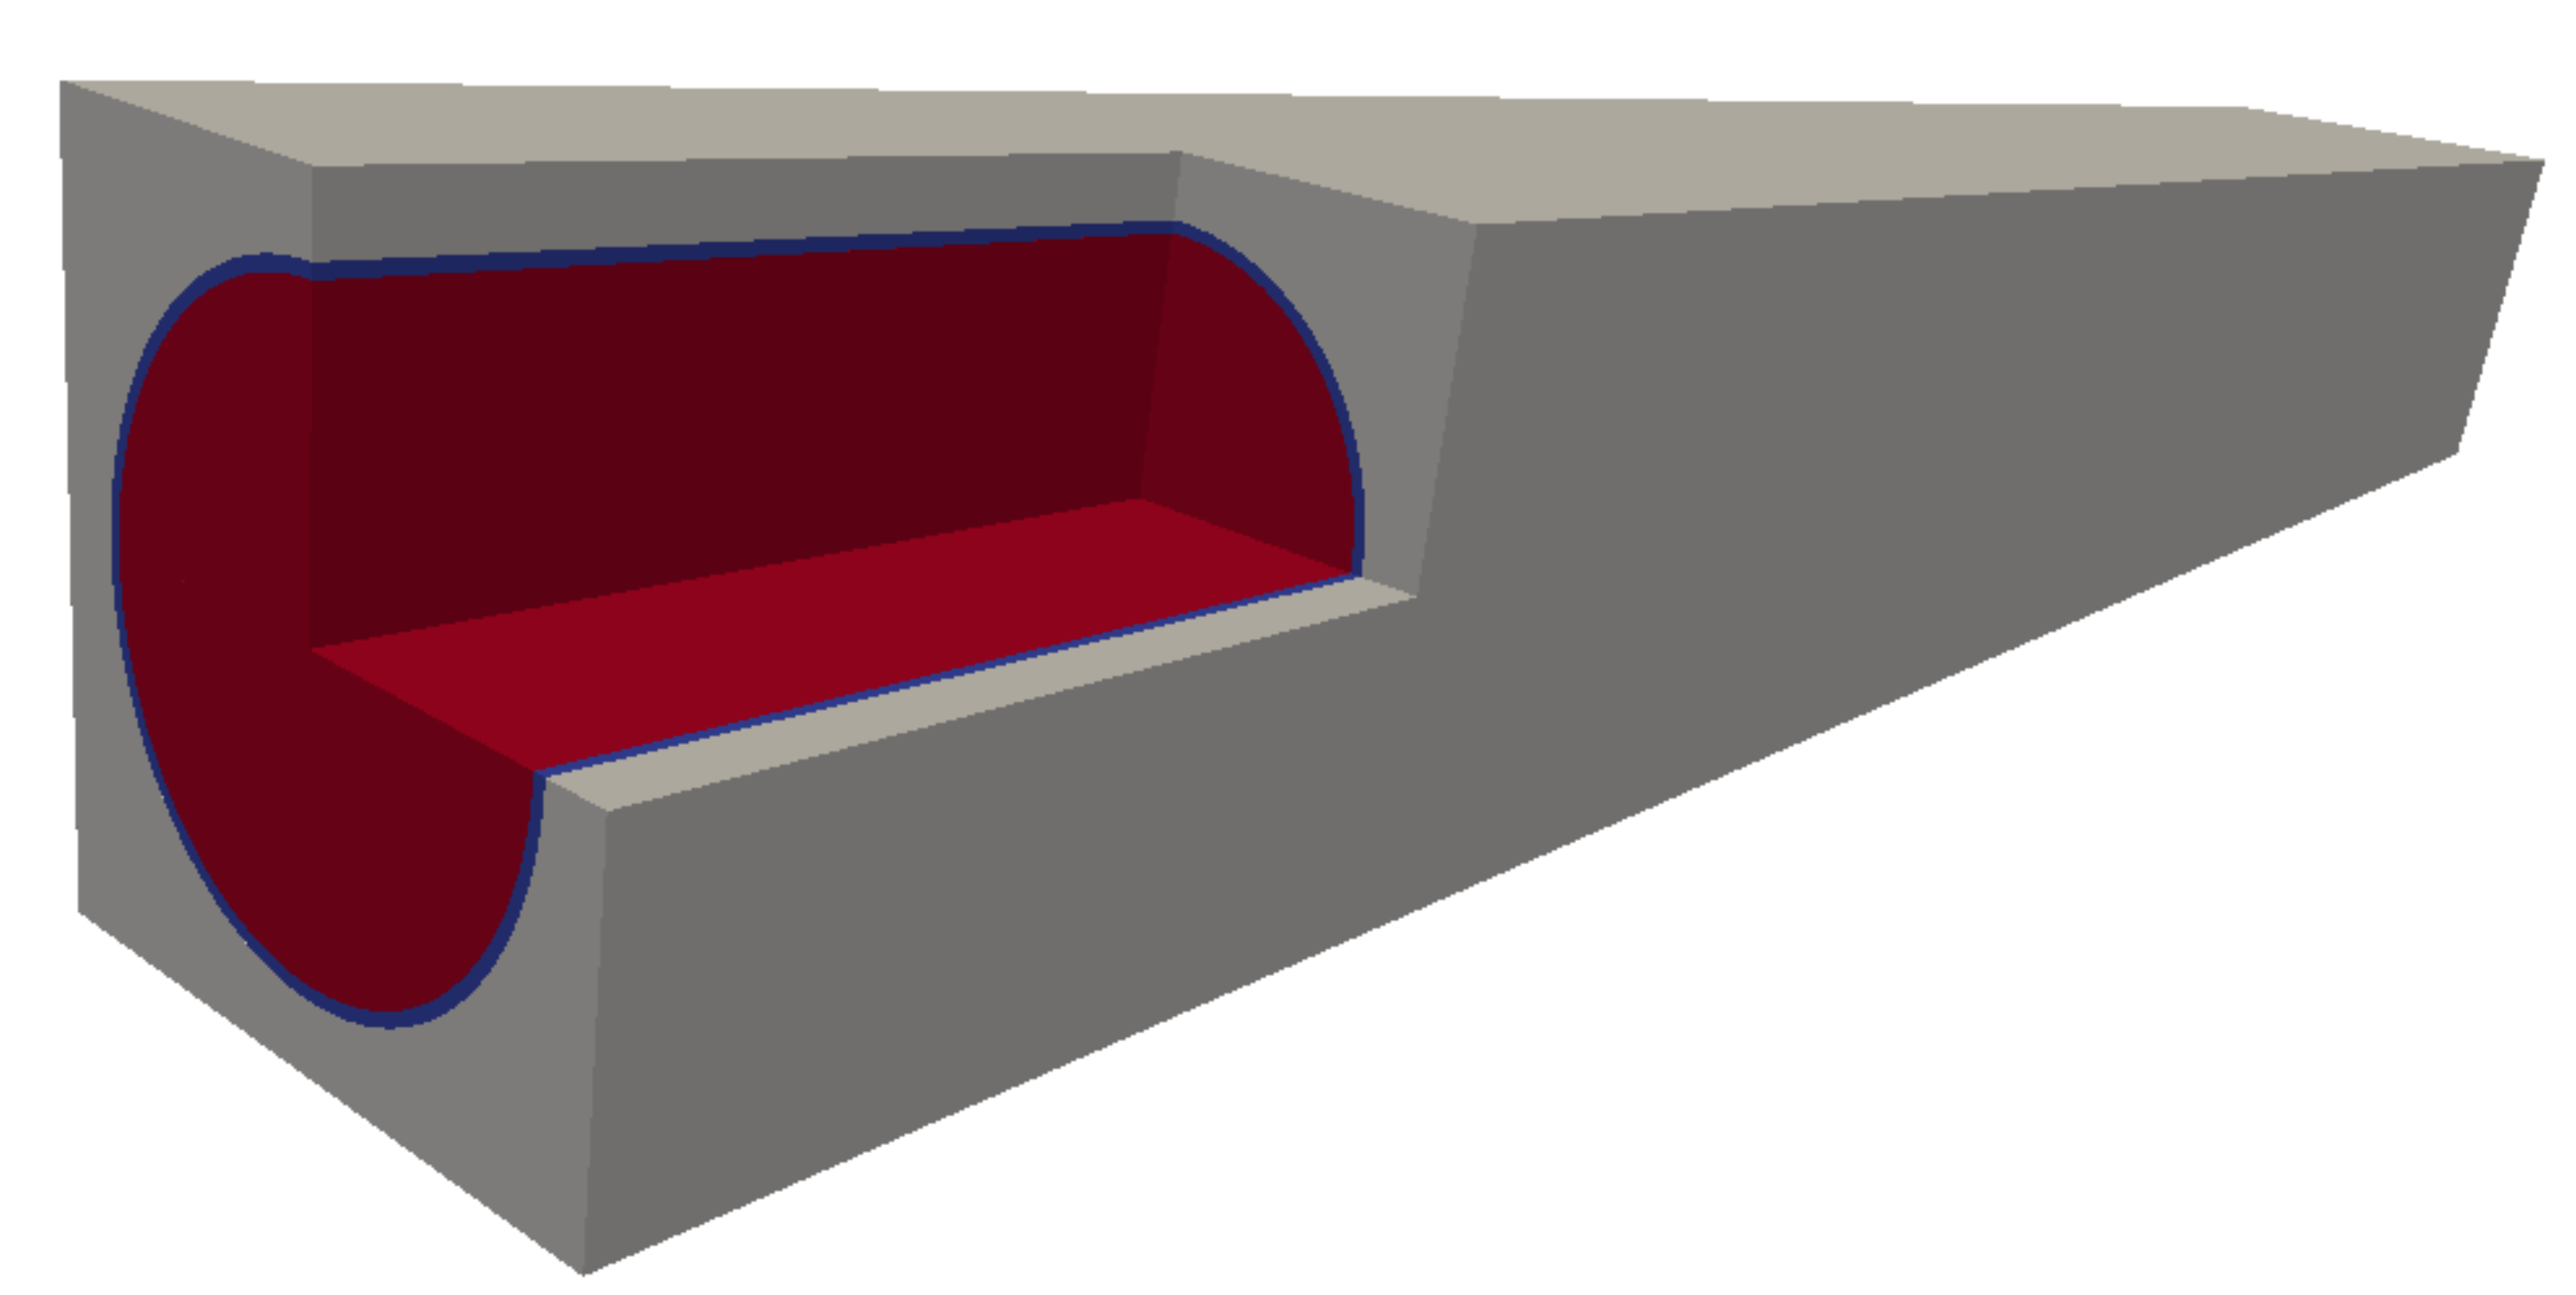
\includegraphics[scale=0.4]{../figuras/all_regions_isometric.png}
  \vspace{0.2cm}
  \raggedright
  \\
  Combustível: hidreto de zircônio e urânio (vermelho).
  \\
  Revestimento: alumínio (azul).
  \\
  Moderador/Refrigerante: água (cinza).
\end{frame}

%-------------------------------------------------
\begin{frame}
  \frametitle{Aplicação}
  \framesubtitle{Modelo \textbf{simplificado} de combustível do reator TRIGA IPR-R1: discretizado}
  \centering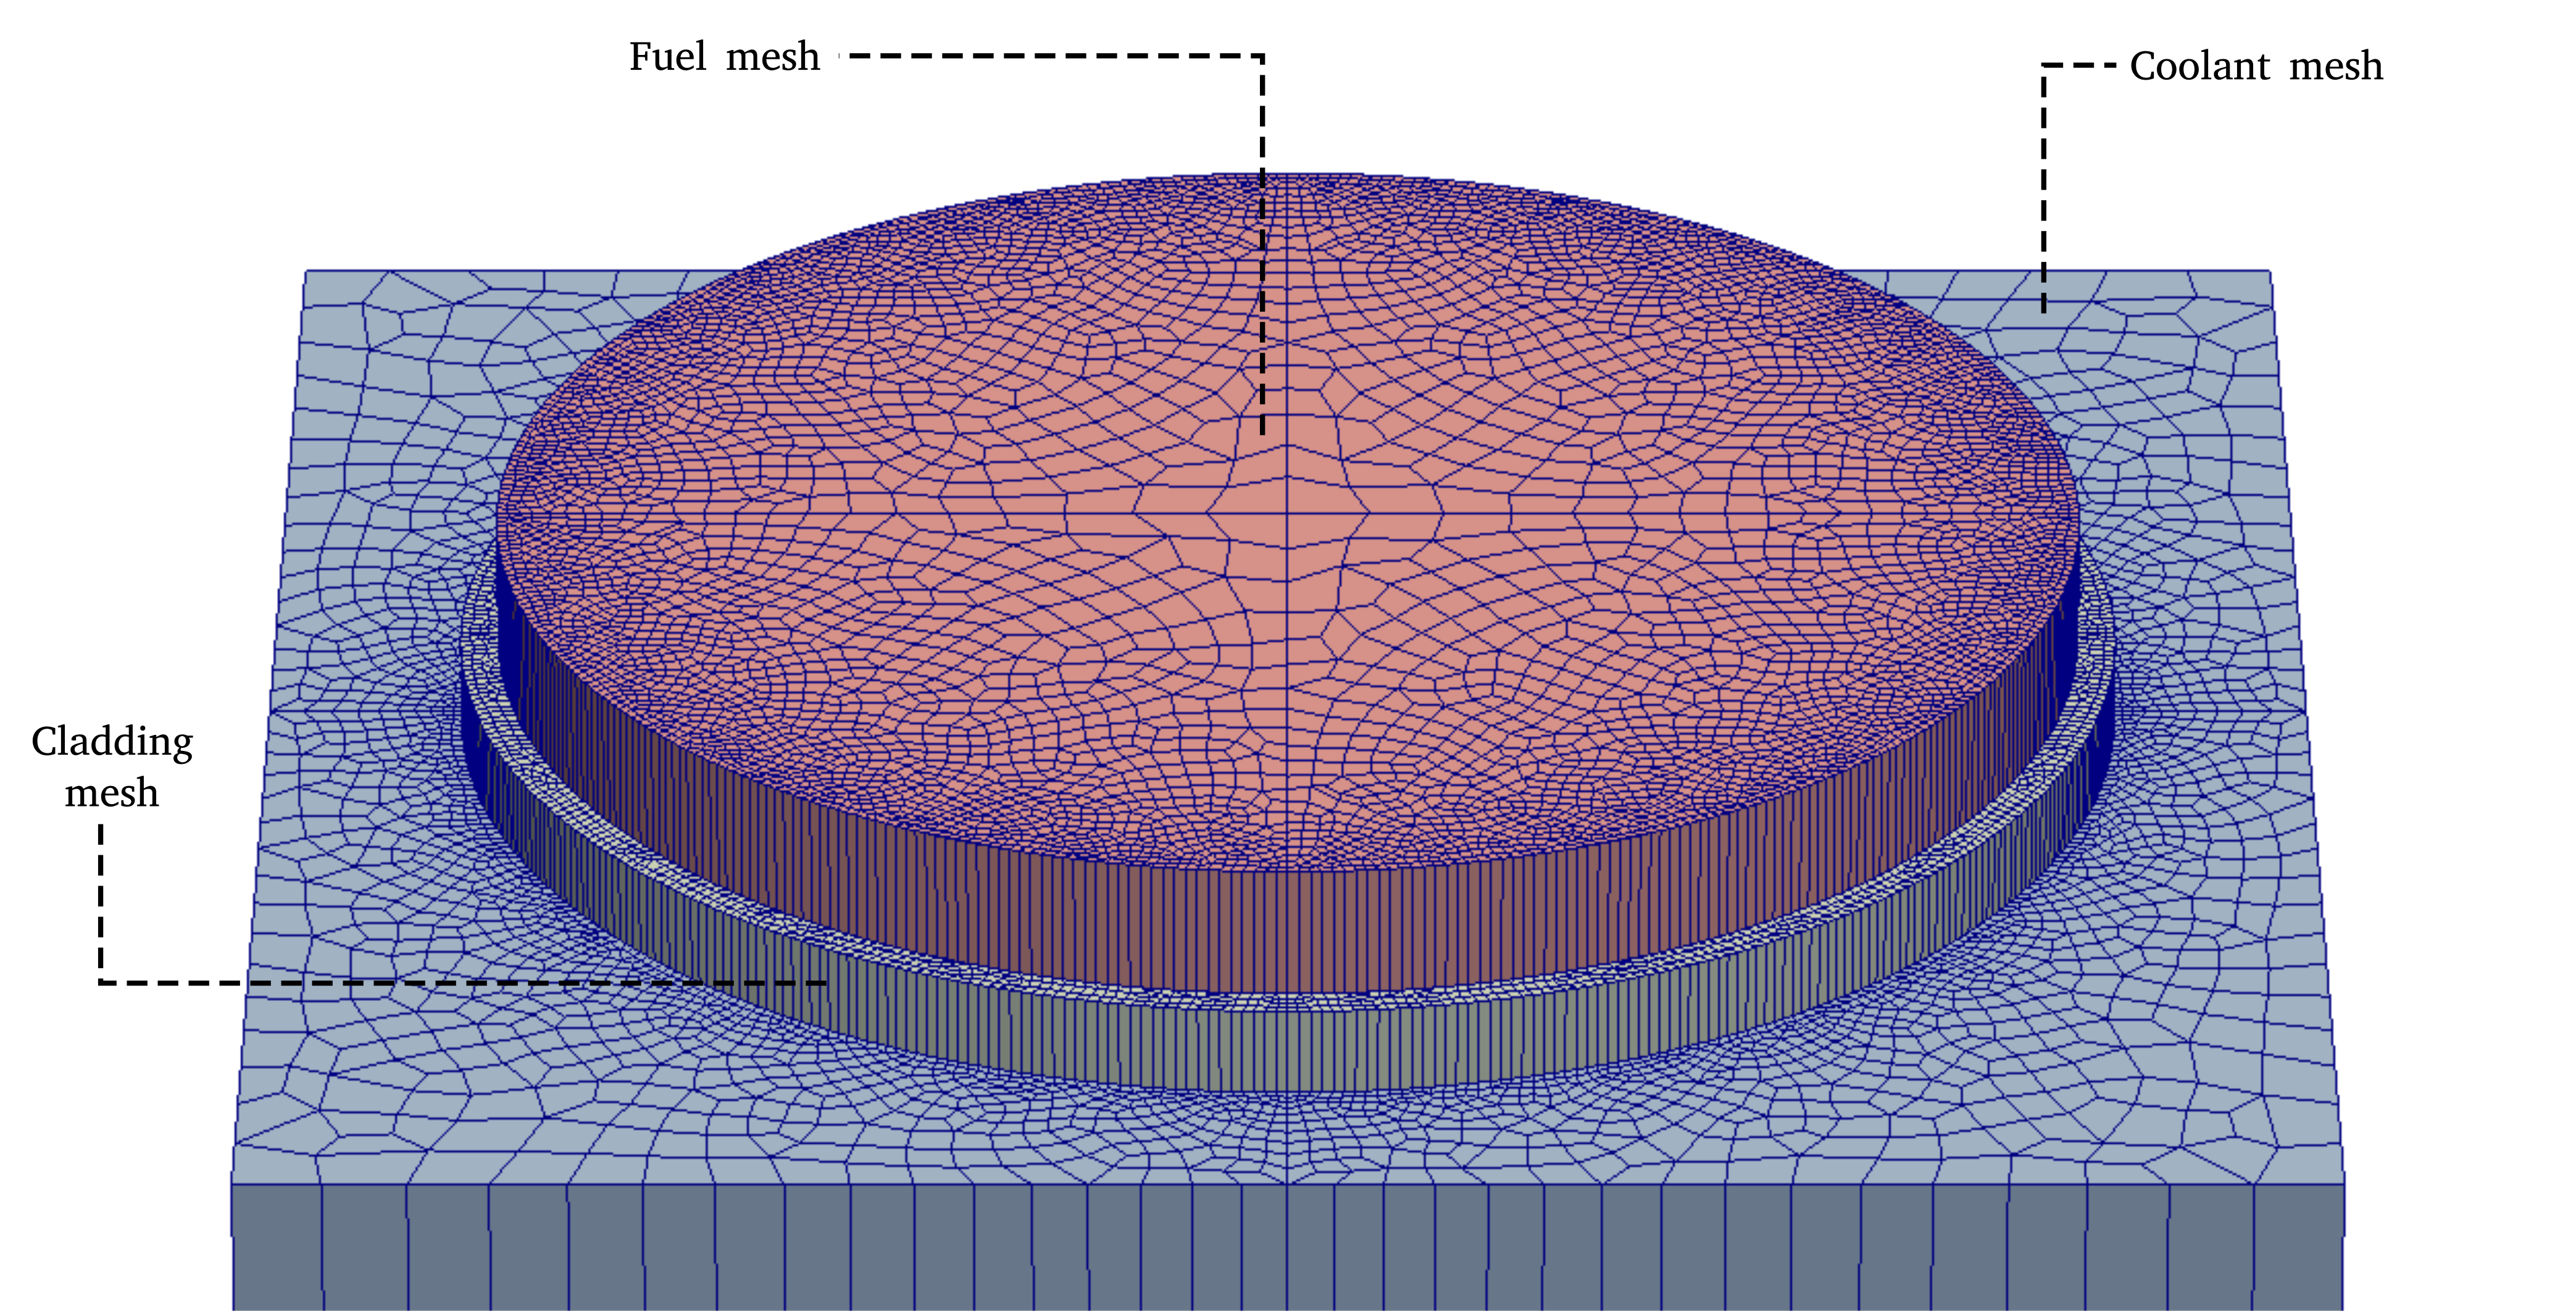
\includegraphics[scale=0.32]{../figuras/regioes_edges_com_legenda_ingles.png}
  \centering
  \vspace{0.2cm}
  $\sim$ 376 mil células.
\end{frame}

%-------------------------------------------------
\begin{frame}
  \frametitle{Aplicação}
  \framesubtitle{Algumas condições iniciais}
  \centering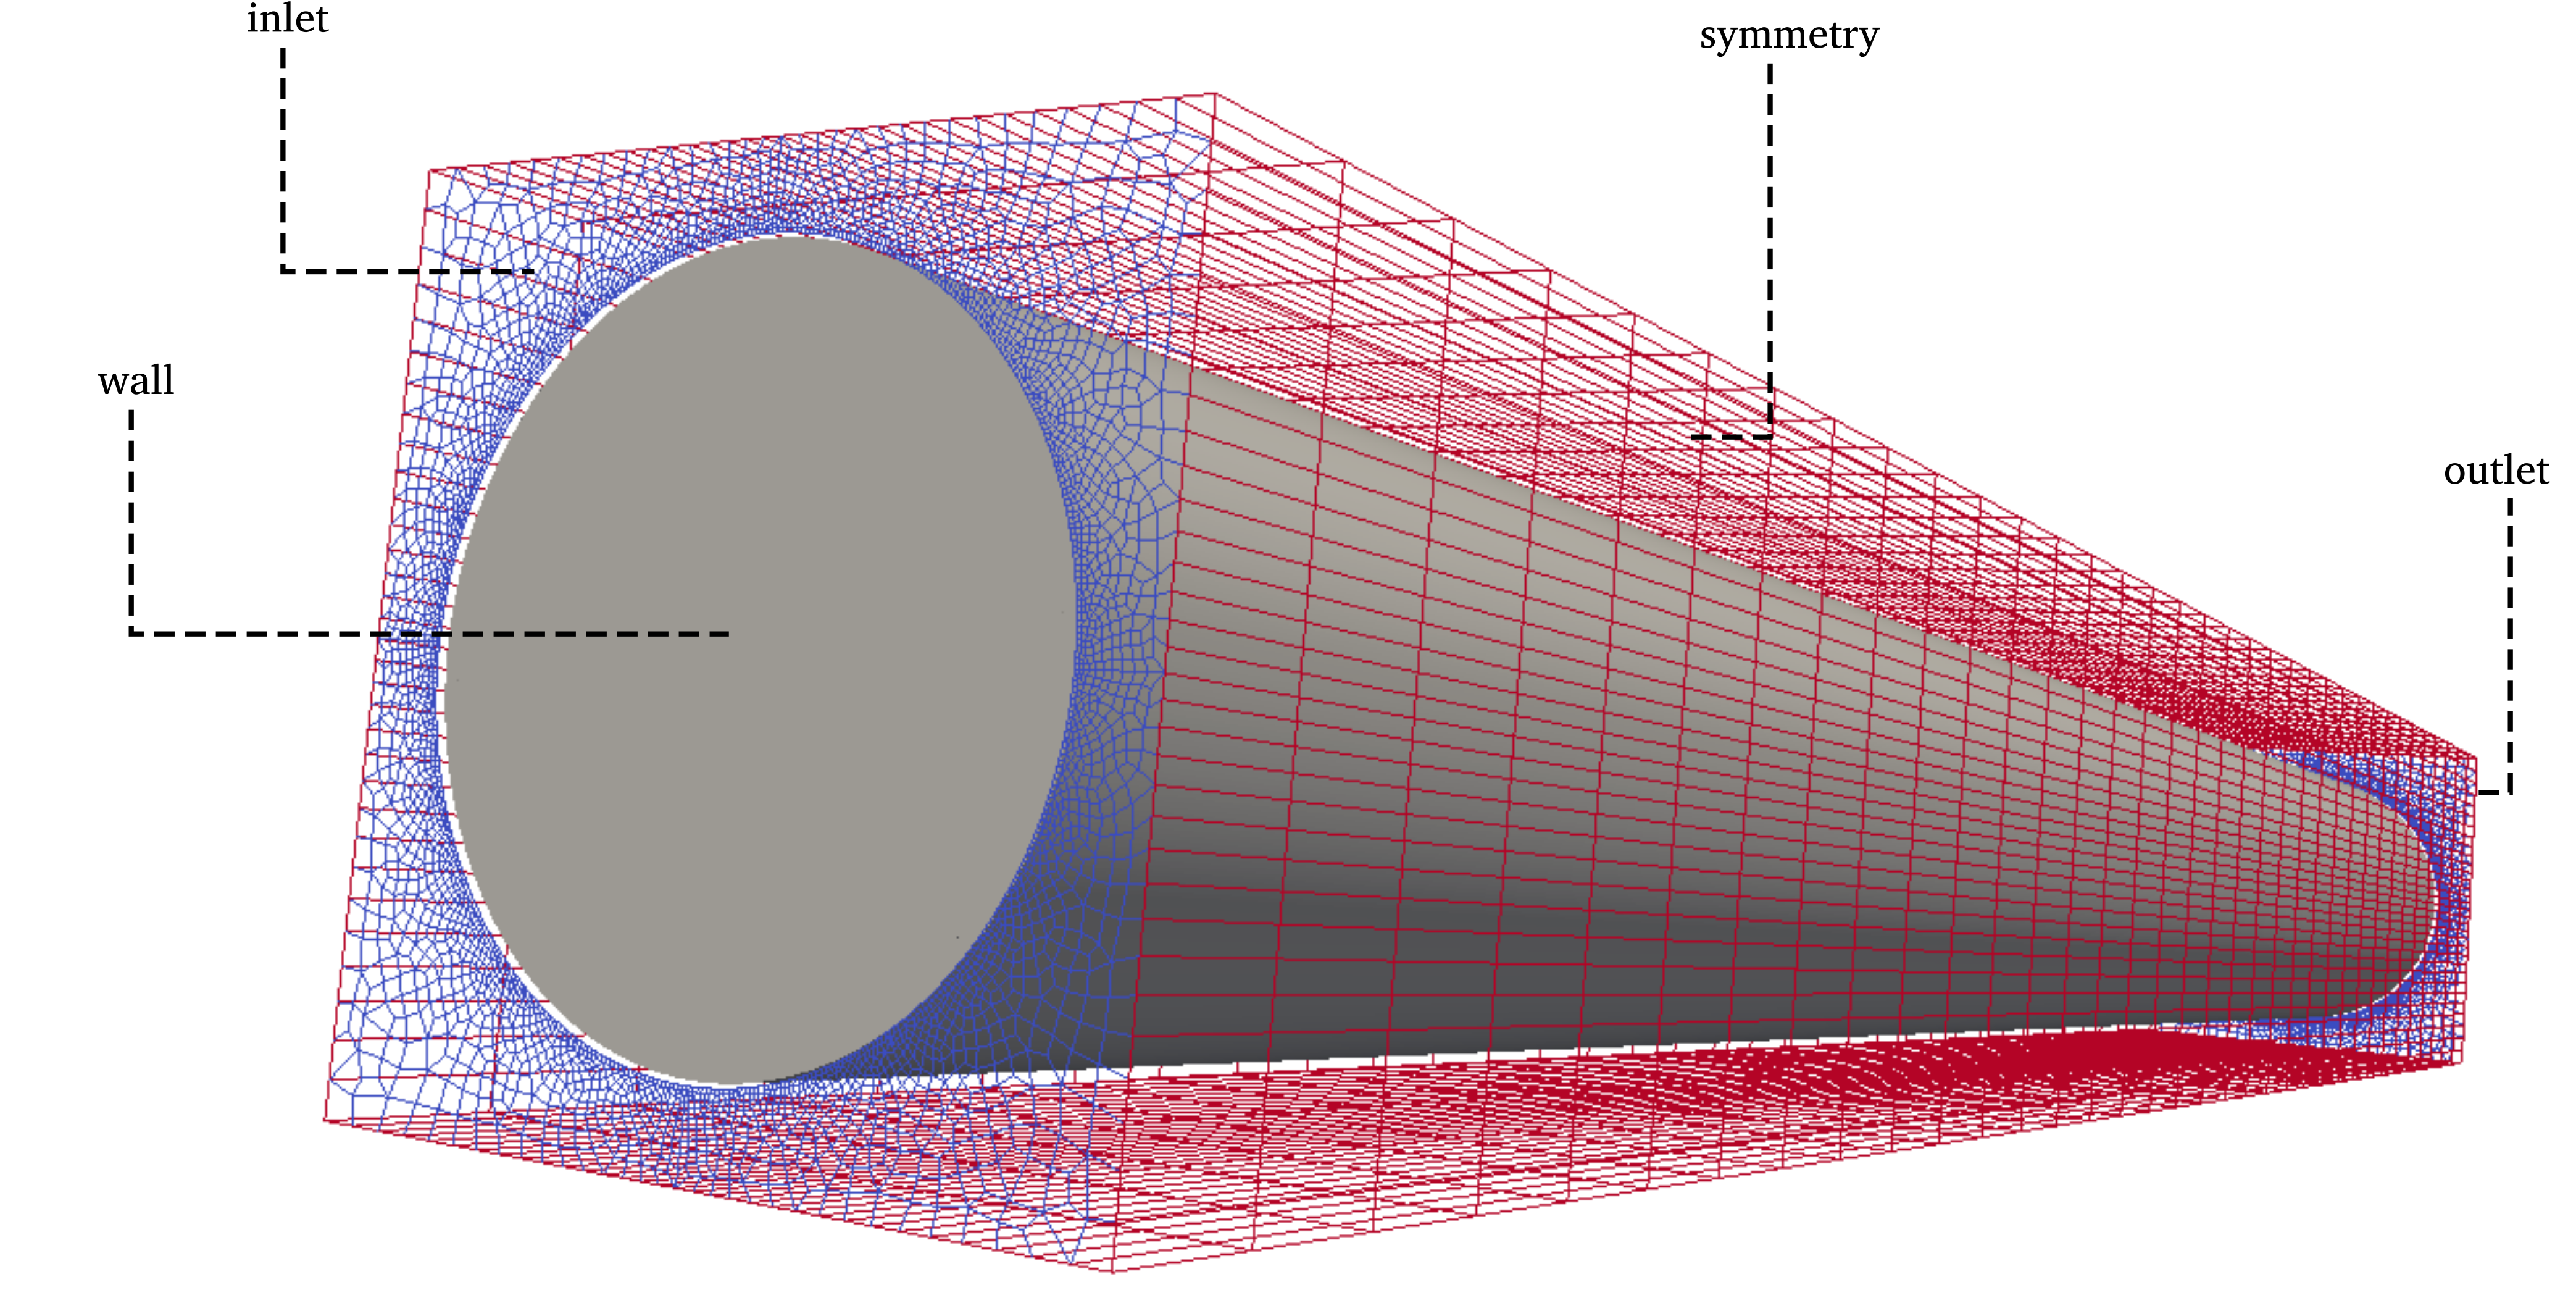
\includegraphics[scale=0.32]{../figuras/inlet_paredes_extremos_wireframe2.png}
  \vspace{0.2cm}
  \raggedright
  \\
  Temperatura de entrada da água: 300 [K] ($\sim27^{\circ}C$).
  \\
  Velocidade do escoamente: $0,1 m/s$.
\end{frame}

%-------------------------------------------------
\begin{frame}
  \frametitle{Aplicação}
  \framesubtitle{Como provar o conceito?}
  Três potências diferentes.
  \\
  \vspace{0.2cm}
  Dois conjuntos de simulações:
%  \\
  \vspace{0.2cm}
  \begin{itemize}
  \item Conjunto 1: simulações \textbf{não-acopladas} em três potências; 
  \item Conjunto 2: simulações \textbf{acopladas} em três potências; 
  \end{itemize}
  \vspace{0.2cm}
  Total de seis simulações.
  
\end{frame}

%-------------------------------------------------
\subsection{Condições iniciais}
\begin{frame}
  \frametitle{Condições iniciais}
  \framesubtitle{Temperaturas médias obtidas da execução do \textit{OpenFOAM} com distribuição homogênea de potência.}
  
    \centering
    Temperaturas médias iniciais.
    \\
    \vspace{0.5cm}
    \label{tab:temp-keff}
    \begin{tabular}{cccc}
      \multicolumn{1}{l}{}         & \multicolumn{3}{c}{Temperaturas [K]}                                                                        \\ \cline{2-4}
      \multicolumn{1}{c}{Potência [kW]} & \multicolumn{1}{c}{Refrigerante} & \multicolumn{1}{c}{Revestimento} & \multicolumn{1}{c}{Combustível}  \\ \hline
      1.98                      & 303,56                         & 327,20                         & 339,80                           \\ \hline
      3.97                      & 307,15                         & 354,54                         & 379,77                           \\ \hline
      7,93                      & 310,09                         & 375,42                         & 422,94                                         
    \end{tabular}
    \vspace{0.5cm}
    \begin{figure}[htb]
    \centering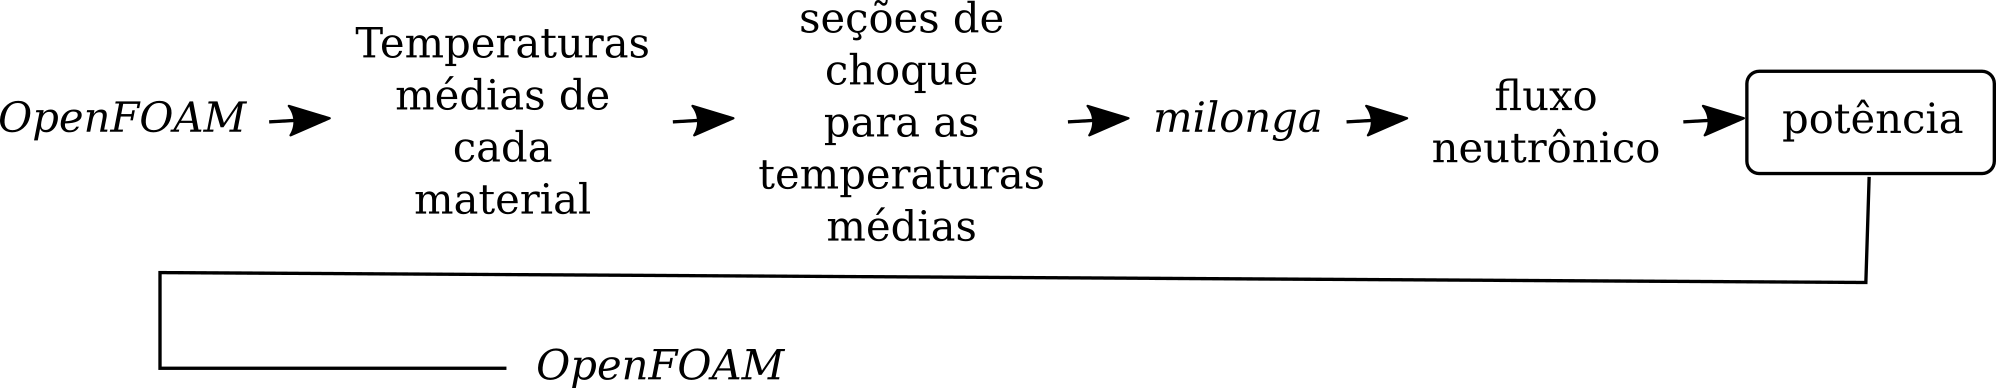
\includegraphics[scale=0.6]{../figuras/initial-condition.png}
    \end{figure}
    \end{frame}

%-------------------------------------------------
\begin{frame}
  \frametitle{Condições iniciais}
  \framesubtitle{Distribuição de potências iniciais}
  %  Fluxo [$\phi/phi_{avg}$].
%  \centering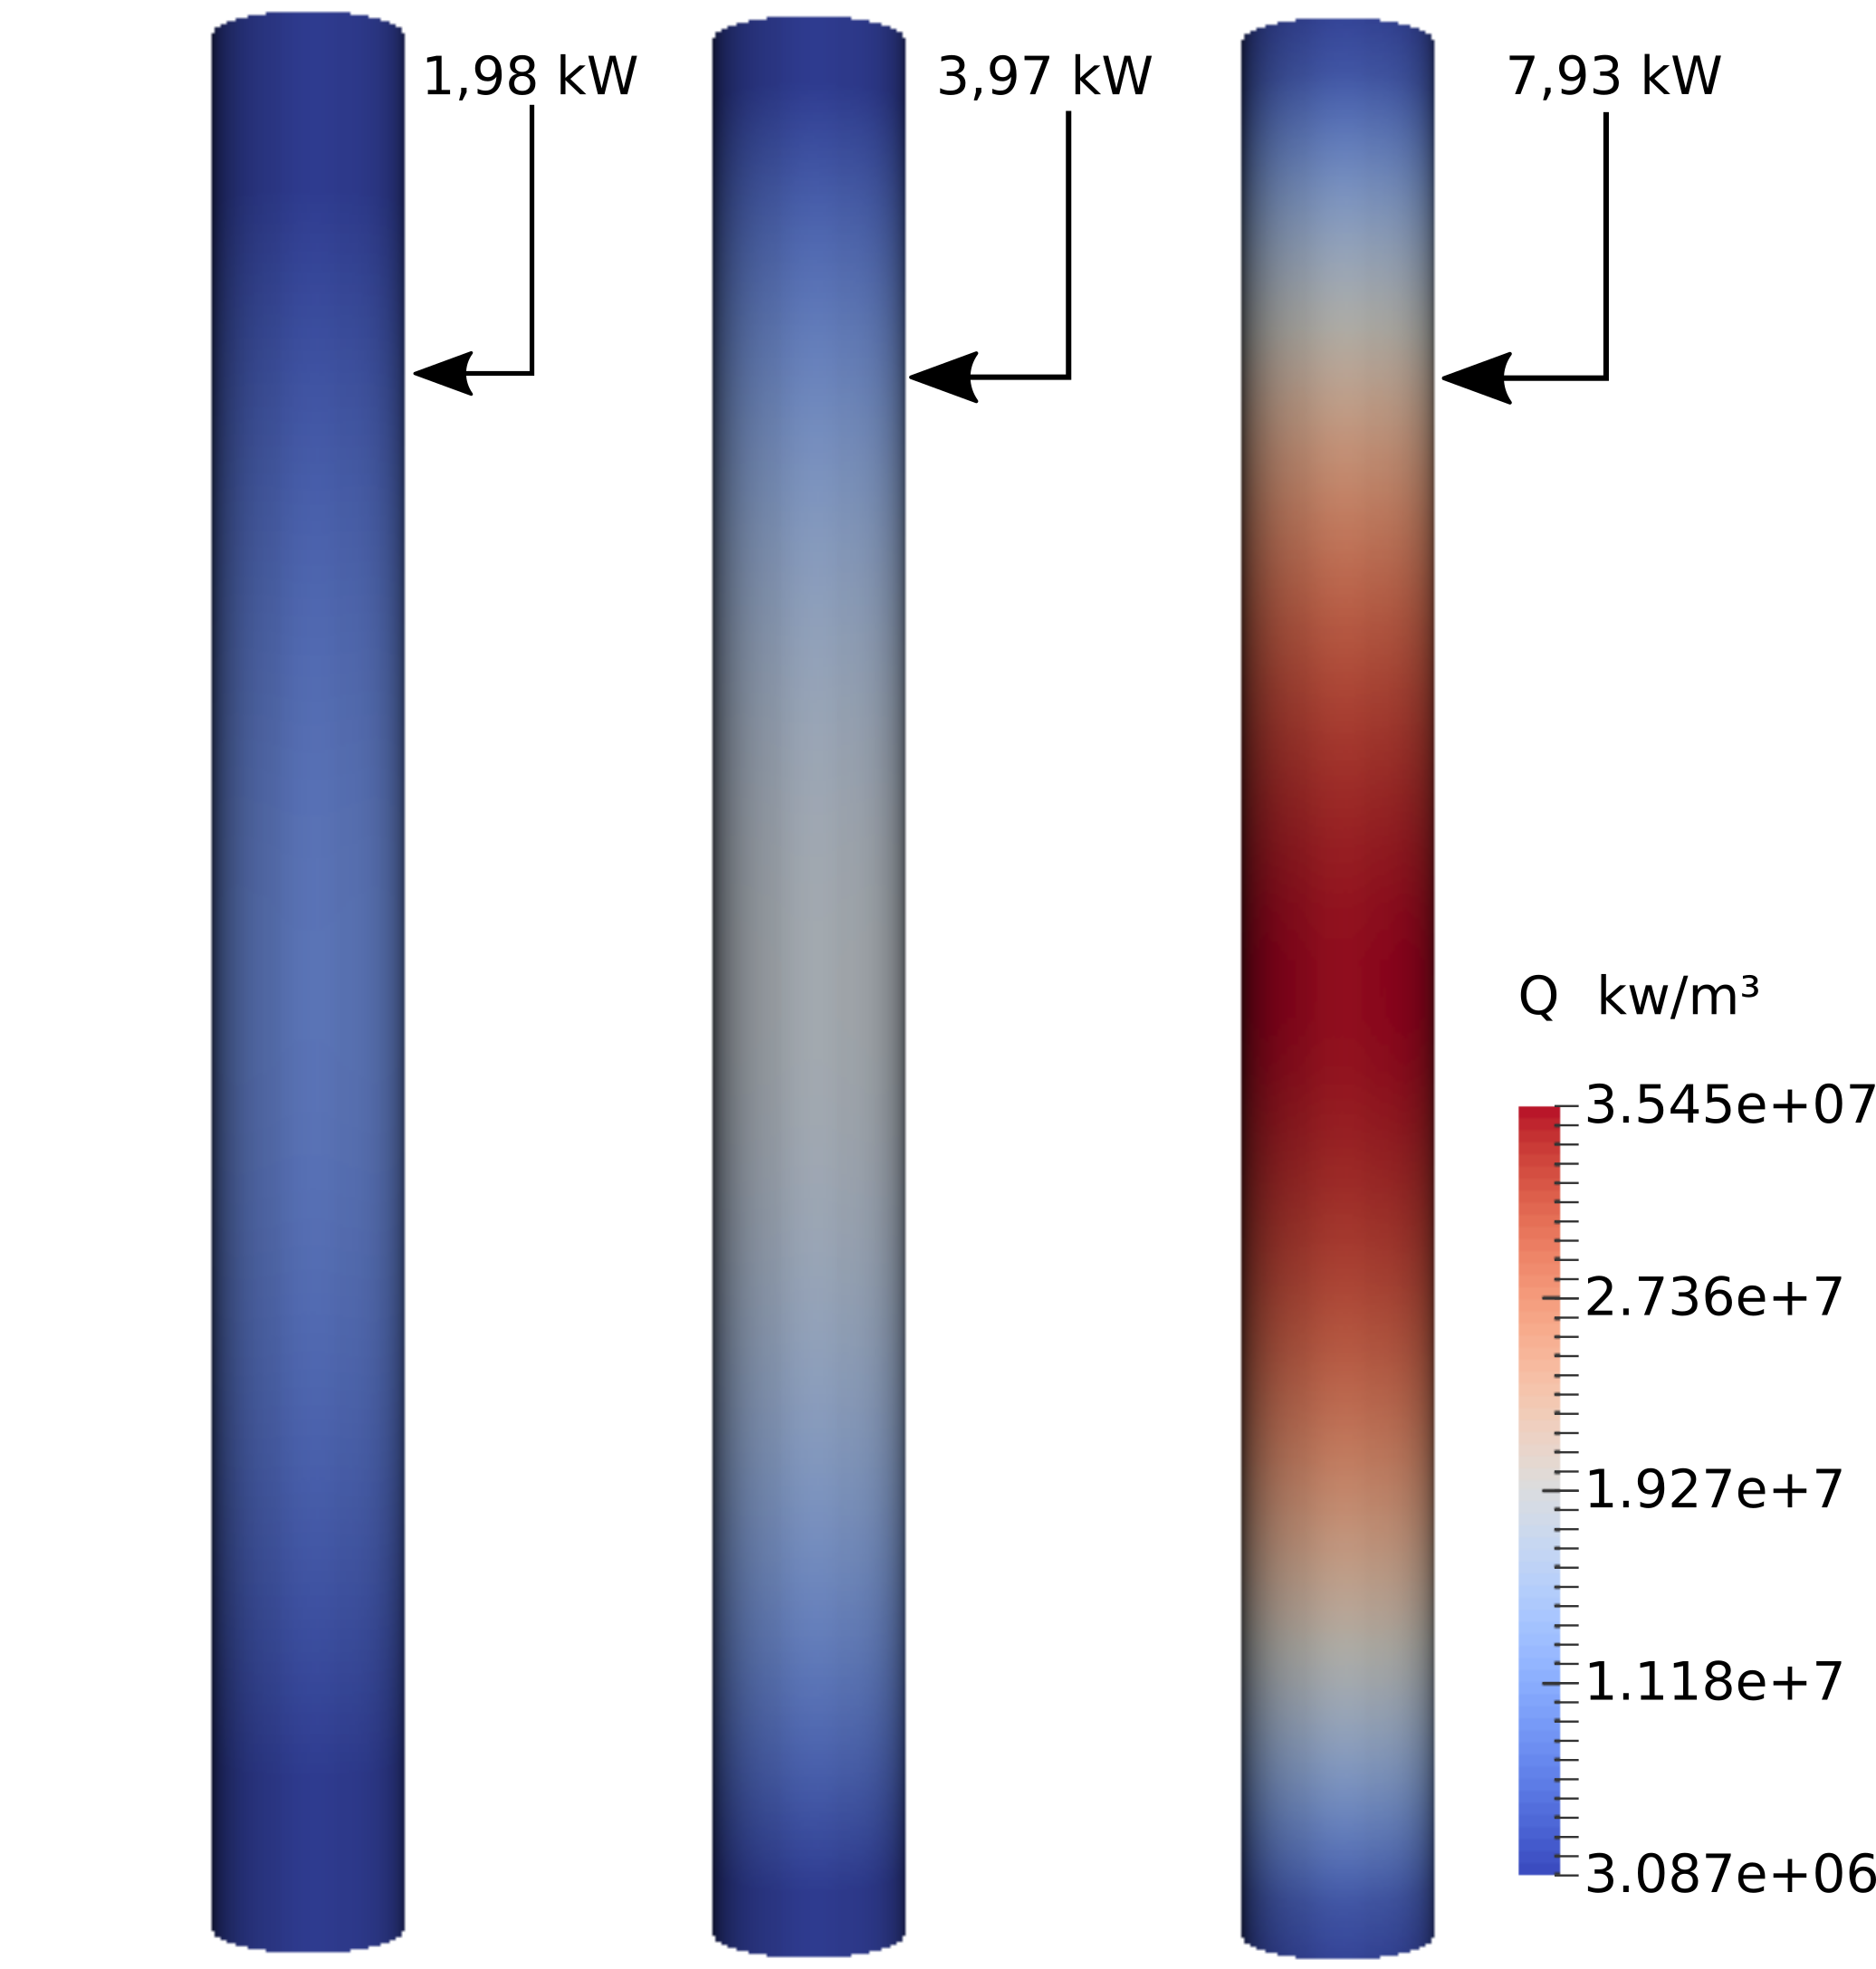
\includegraphics[width=\textwidth, height=7.0cm]{../figuras/Q_fuel_all_NC.png}
  \centering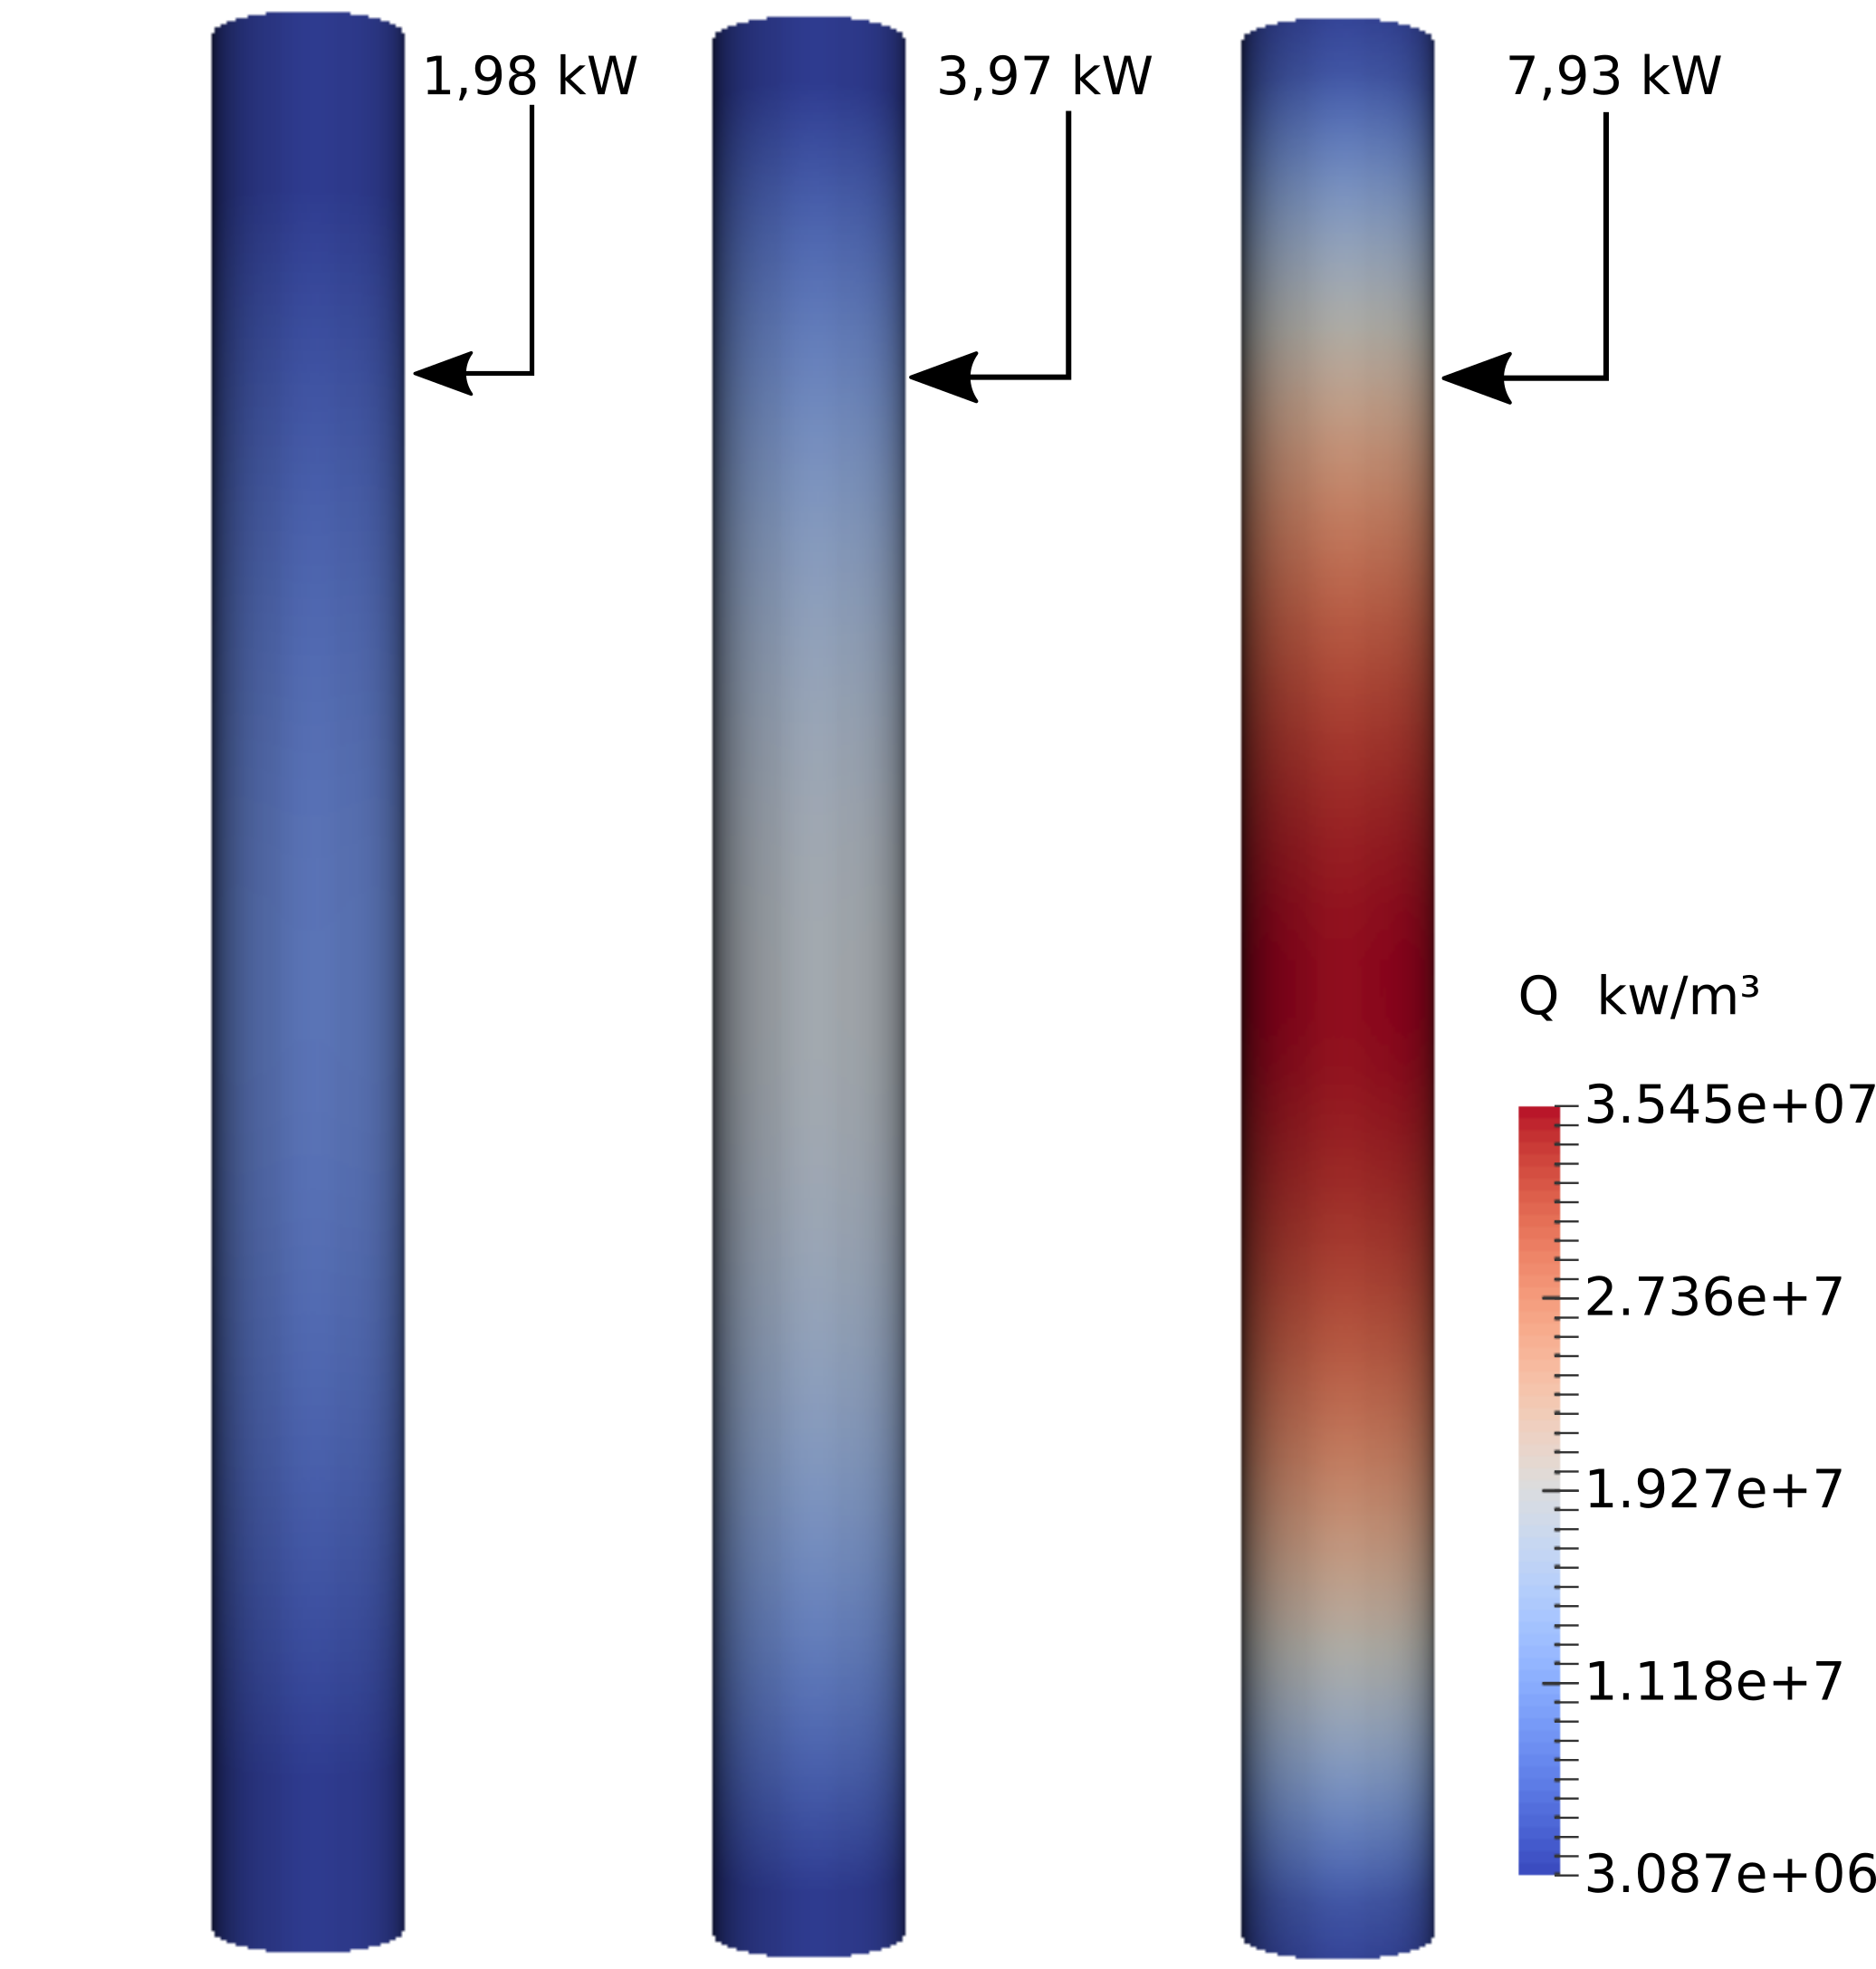
\includegraphics[scale=0.4]{../figuras/Q_fuel_all_NC.png}
\end{frame}

\section{Resultados}
%-------------------------------------------------
\subsection{Gráficos}
\begin{frame}
  \frametitle{Resultados}
  \framesubtitle{Fluxo neutrônico: distribuição axial ($7,93 kW$)}
  %  Fluxo [$\phi/phi_{avg}$].
  \centering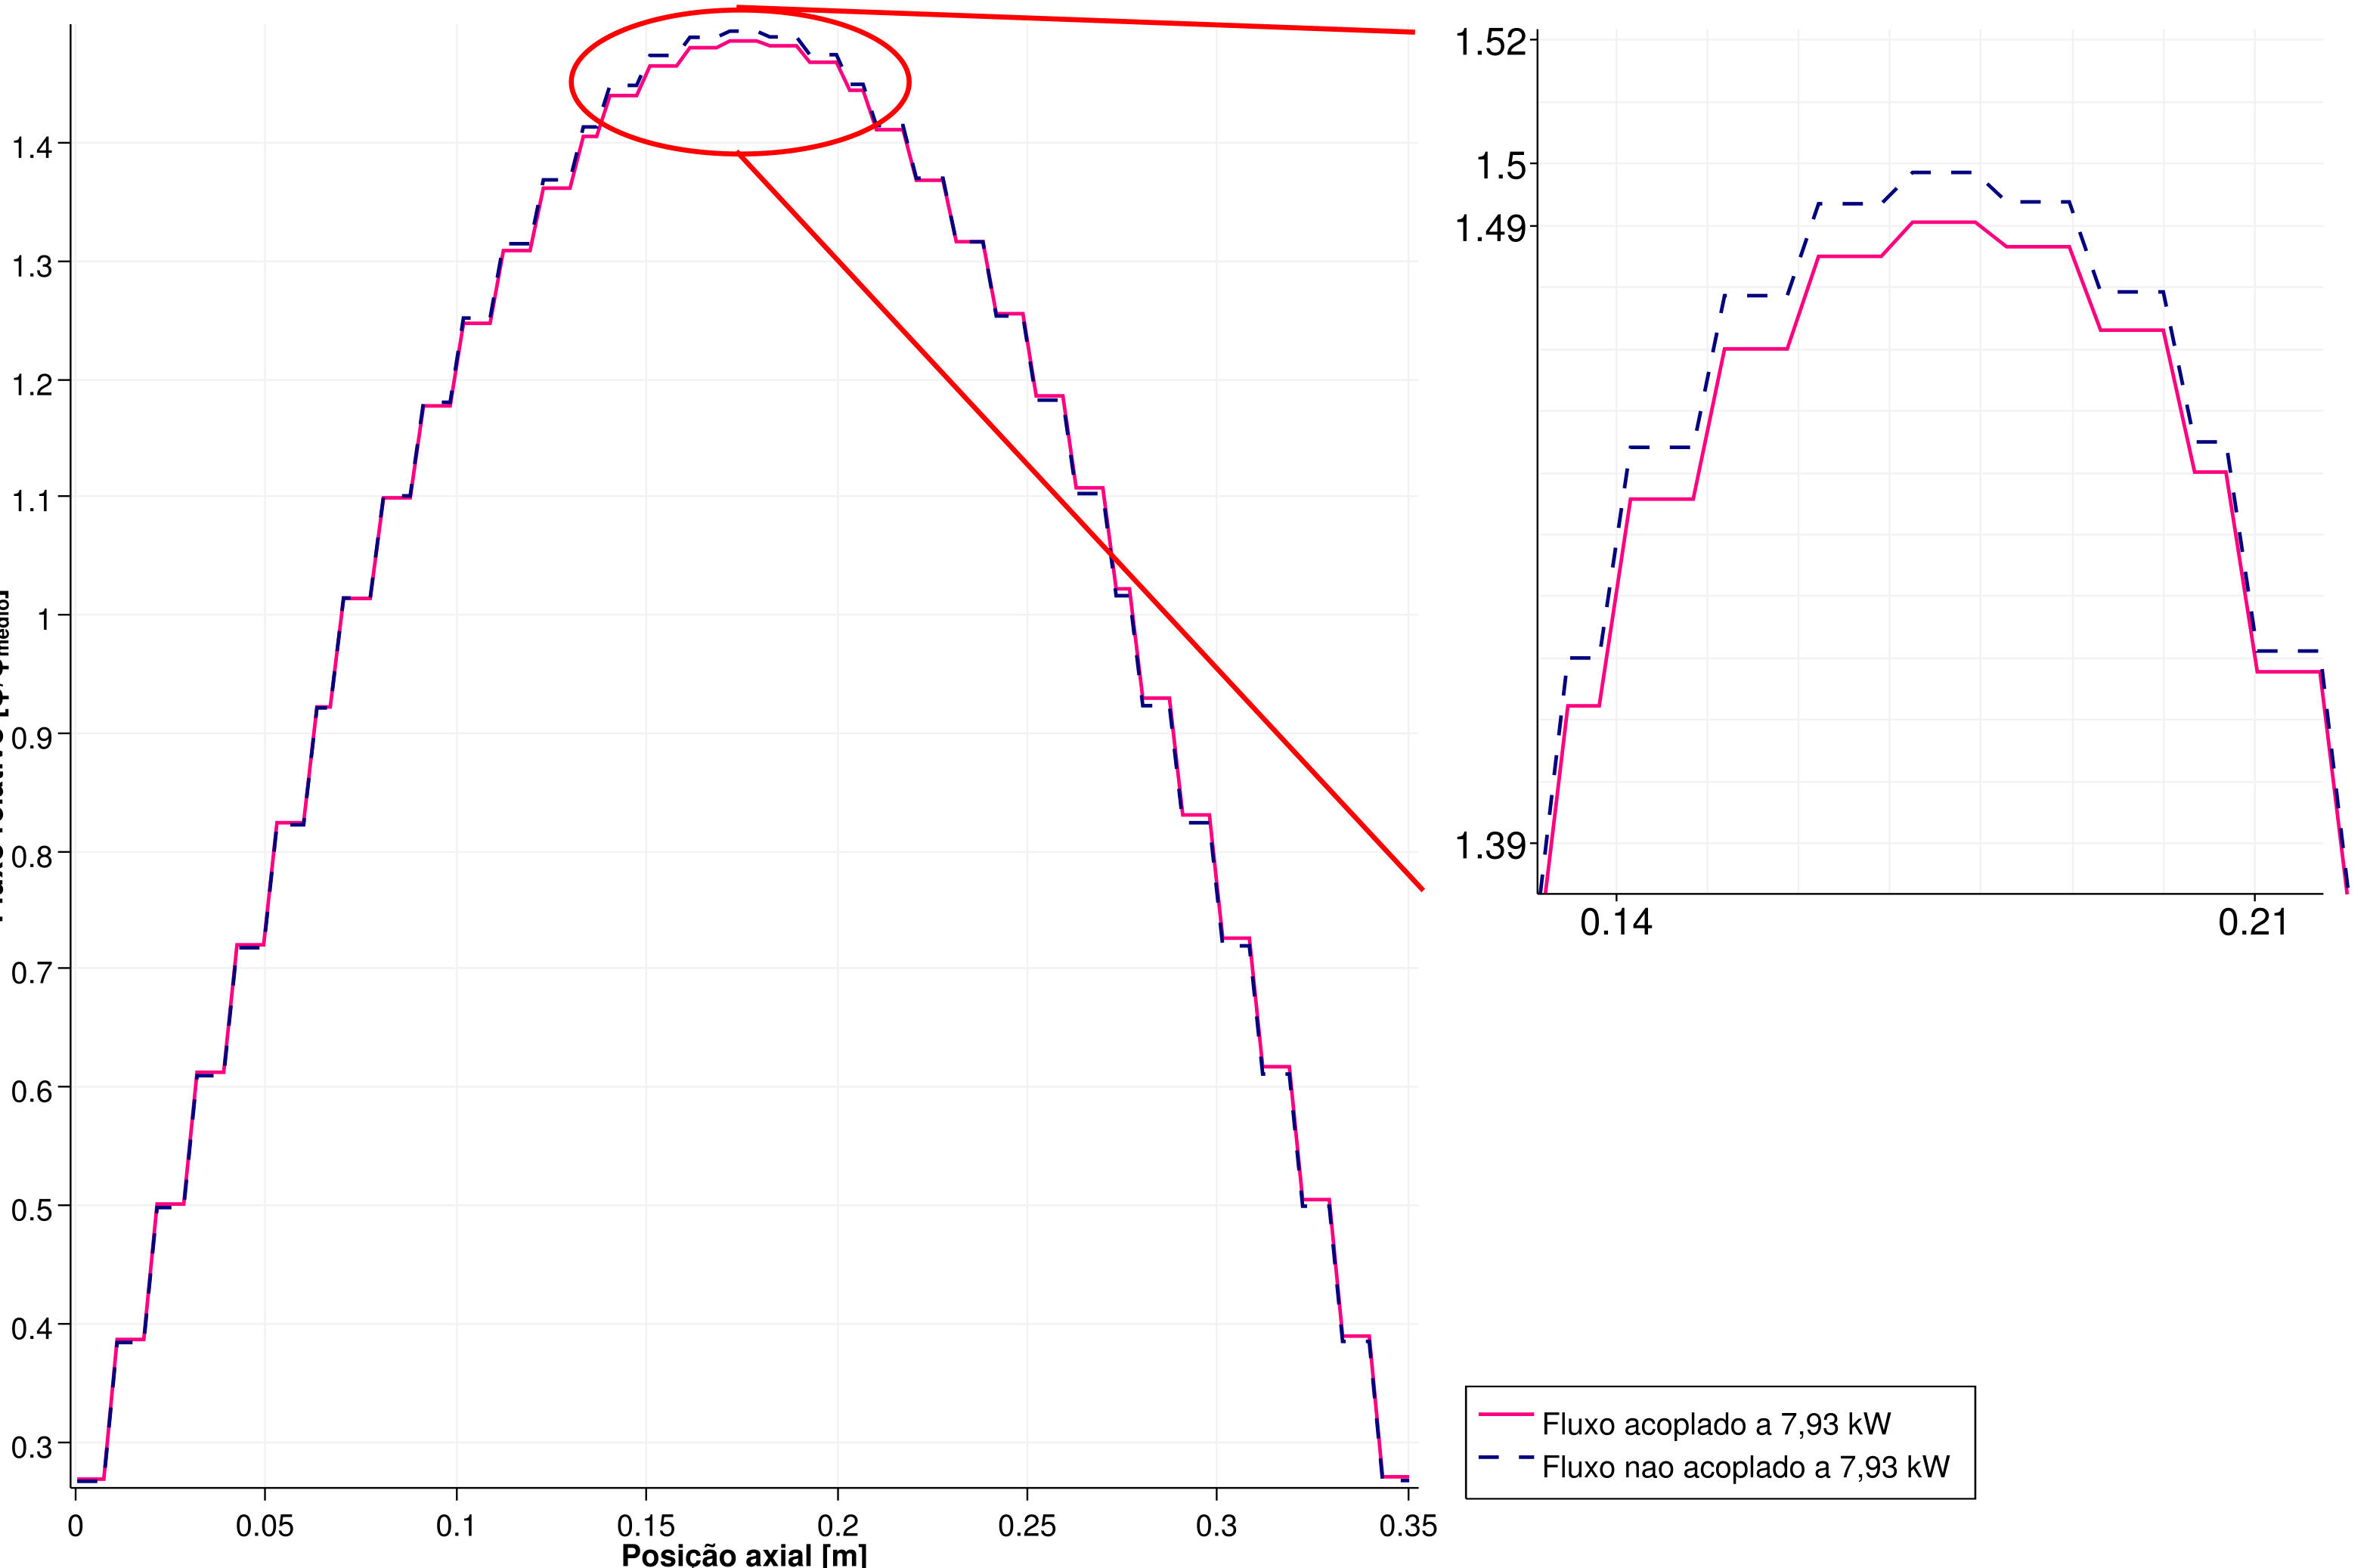
\includegraphics[width=\textwidth, height=7.0cm]{../figuras/Flux_rel_z_200_port_trabalhado.png}
  \label{fig:flux200z}
\end{frame}

%-------------------------------------------------
%\subsection{Gráficos}
\begin{frame}
  \frametitle{Resultados}
  \framesubtitle{Fluxo neutrônico: distribuição radial ($7,93 kW$)}
%  Fluxo [$\phi/phi_{avg}$].
  \centering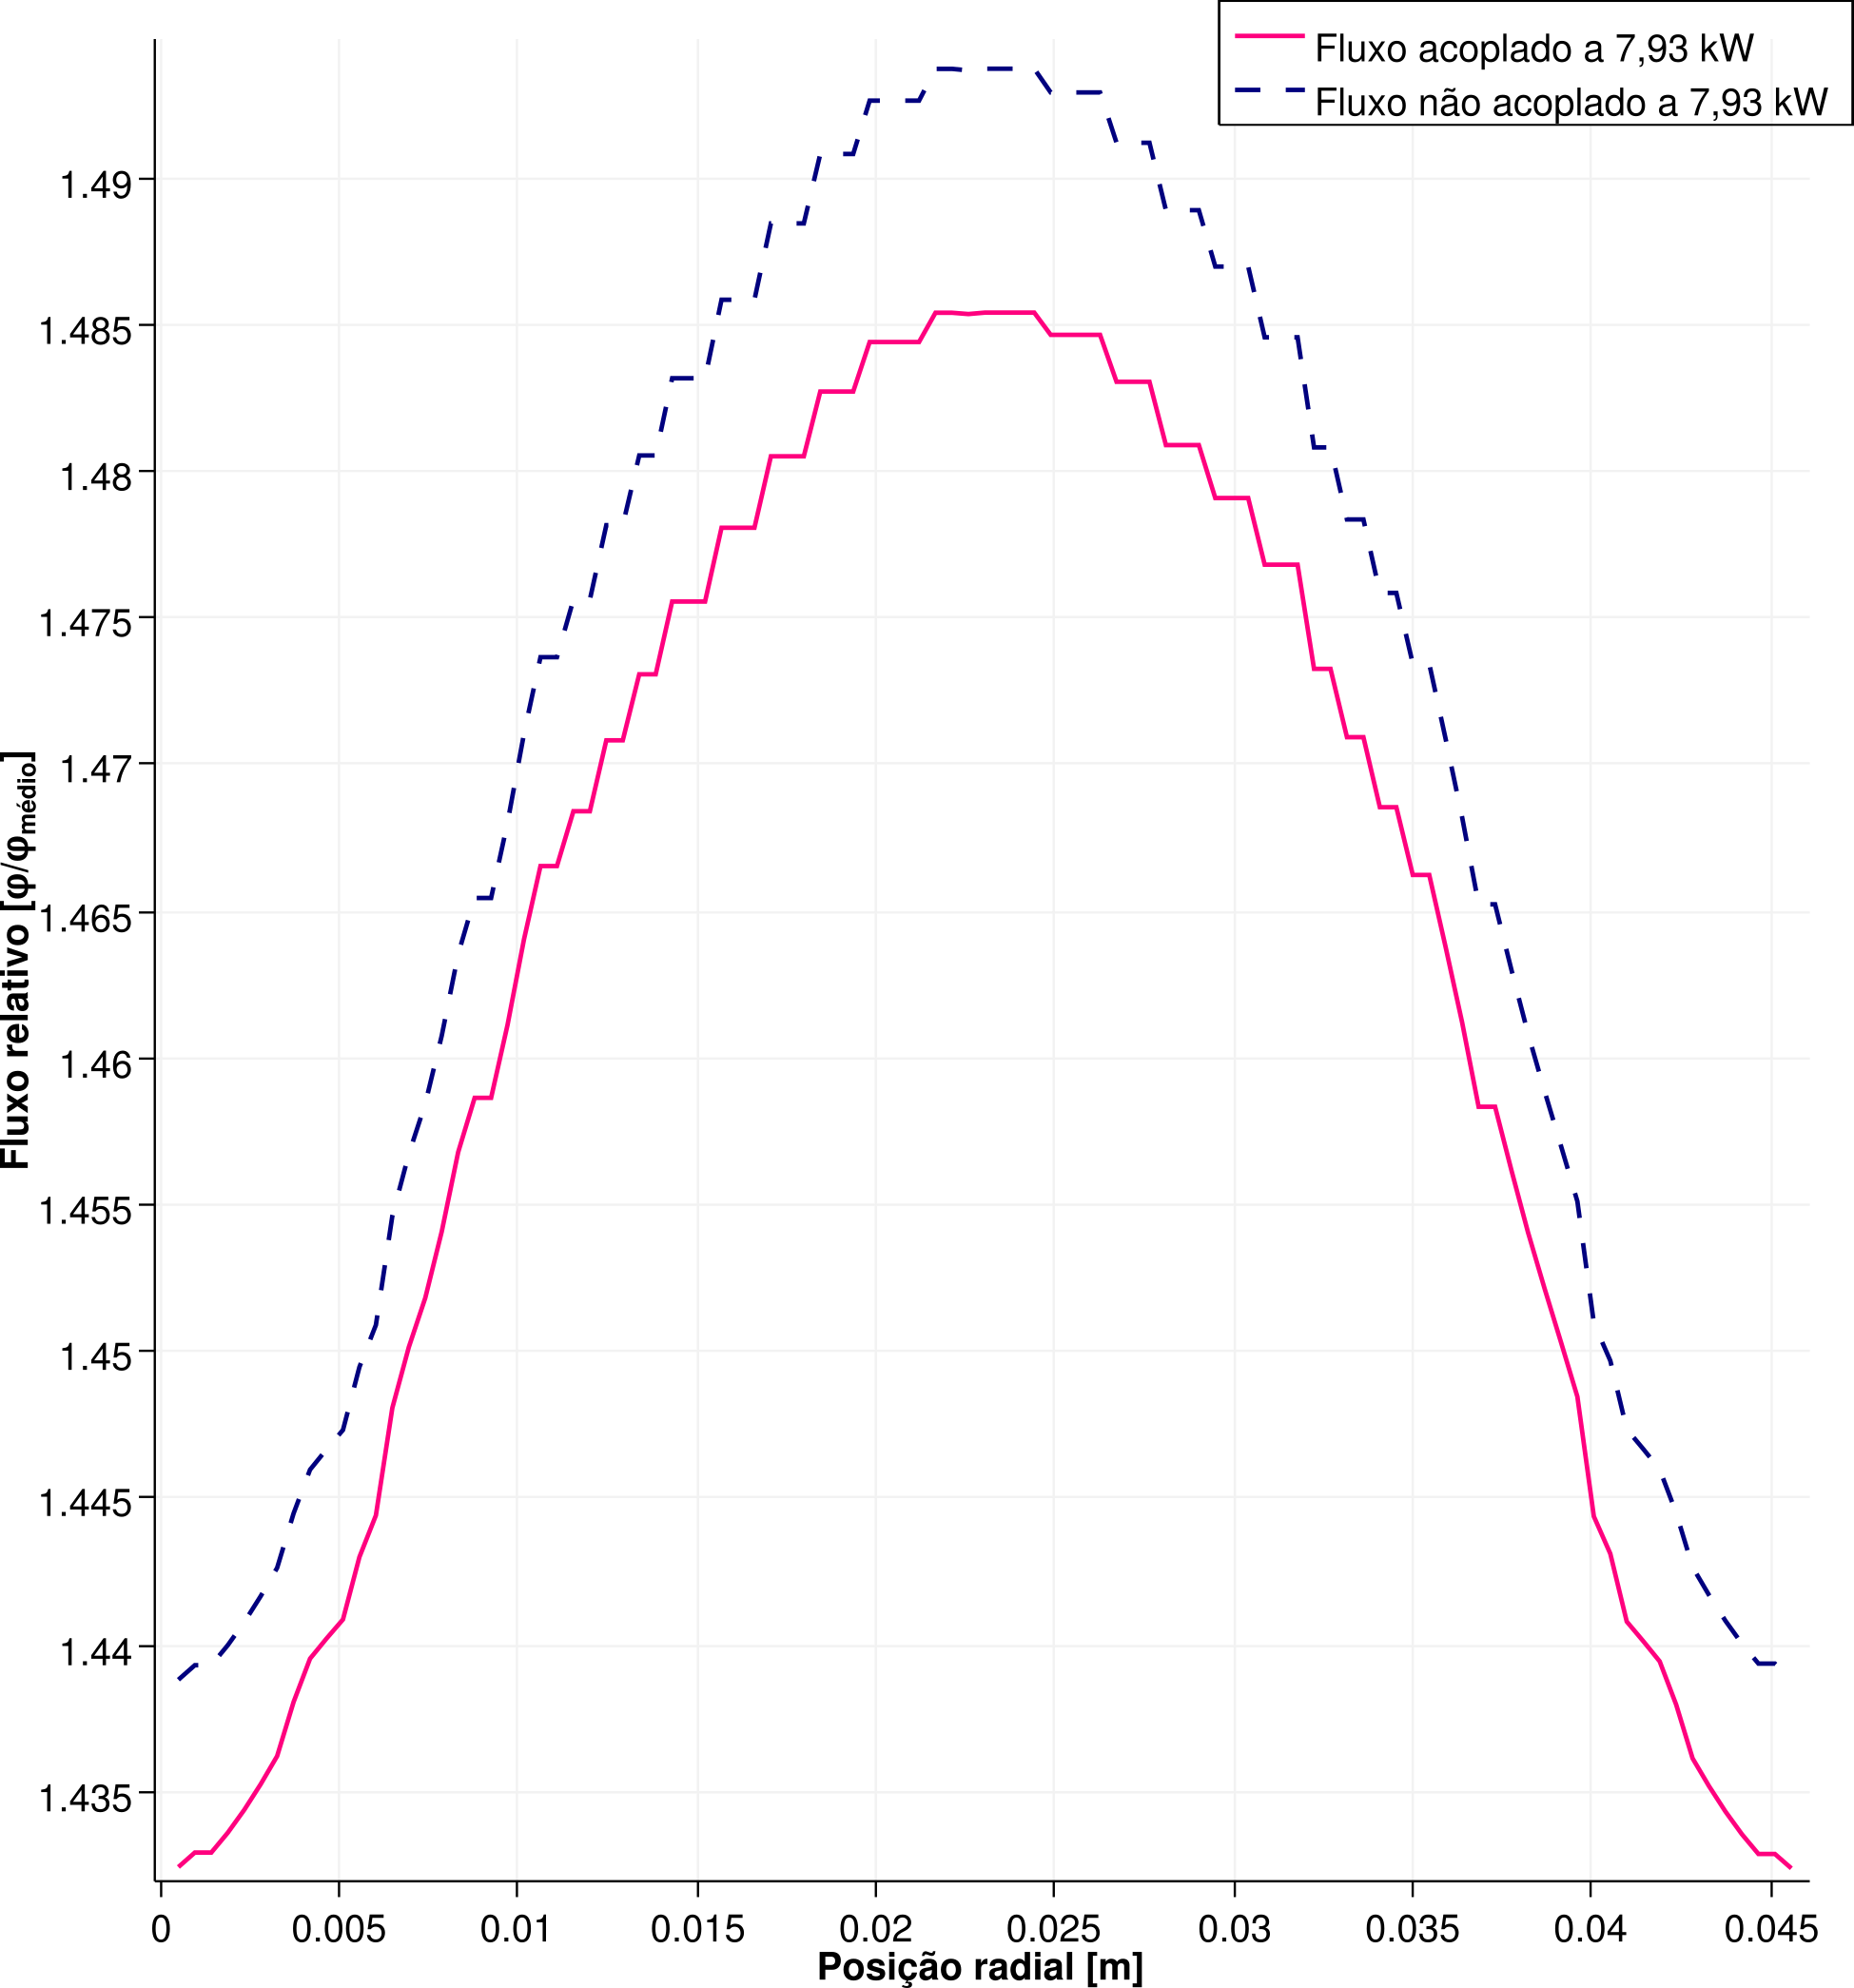
\includegraphics[width=\textwidth, height=7.0cm]{../figuras/Flux_rel_x_200_port.png}
  \label{fig:flux200x}
\end{frame}

%-------------------------------------------------
%\subsection{Gráficos}
\begin{frame}
  \frametitle{Resultados}
  \framesubtitle{Potência: distribuição axial}
%  Distribuição de potência [$kW/m^3$].
  \centering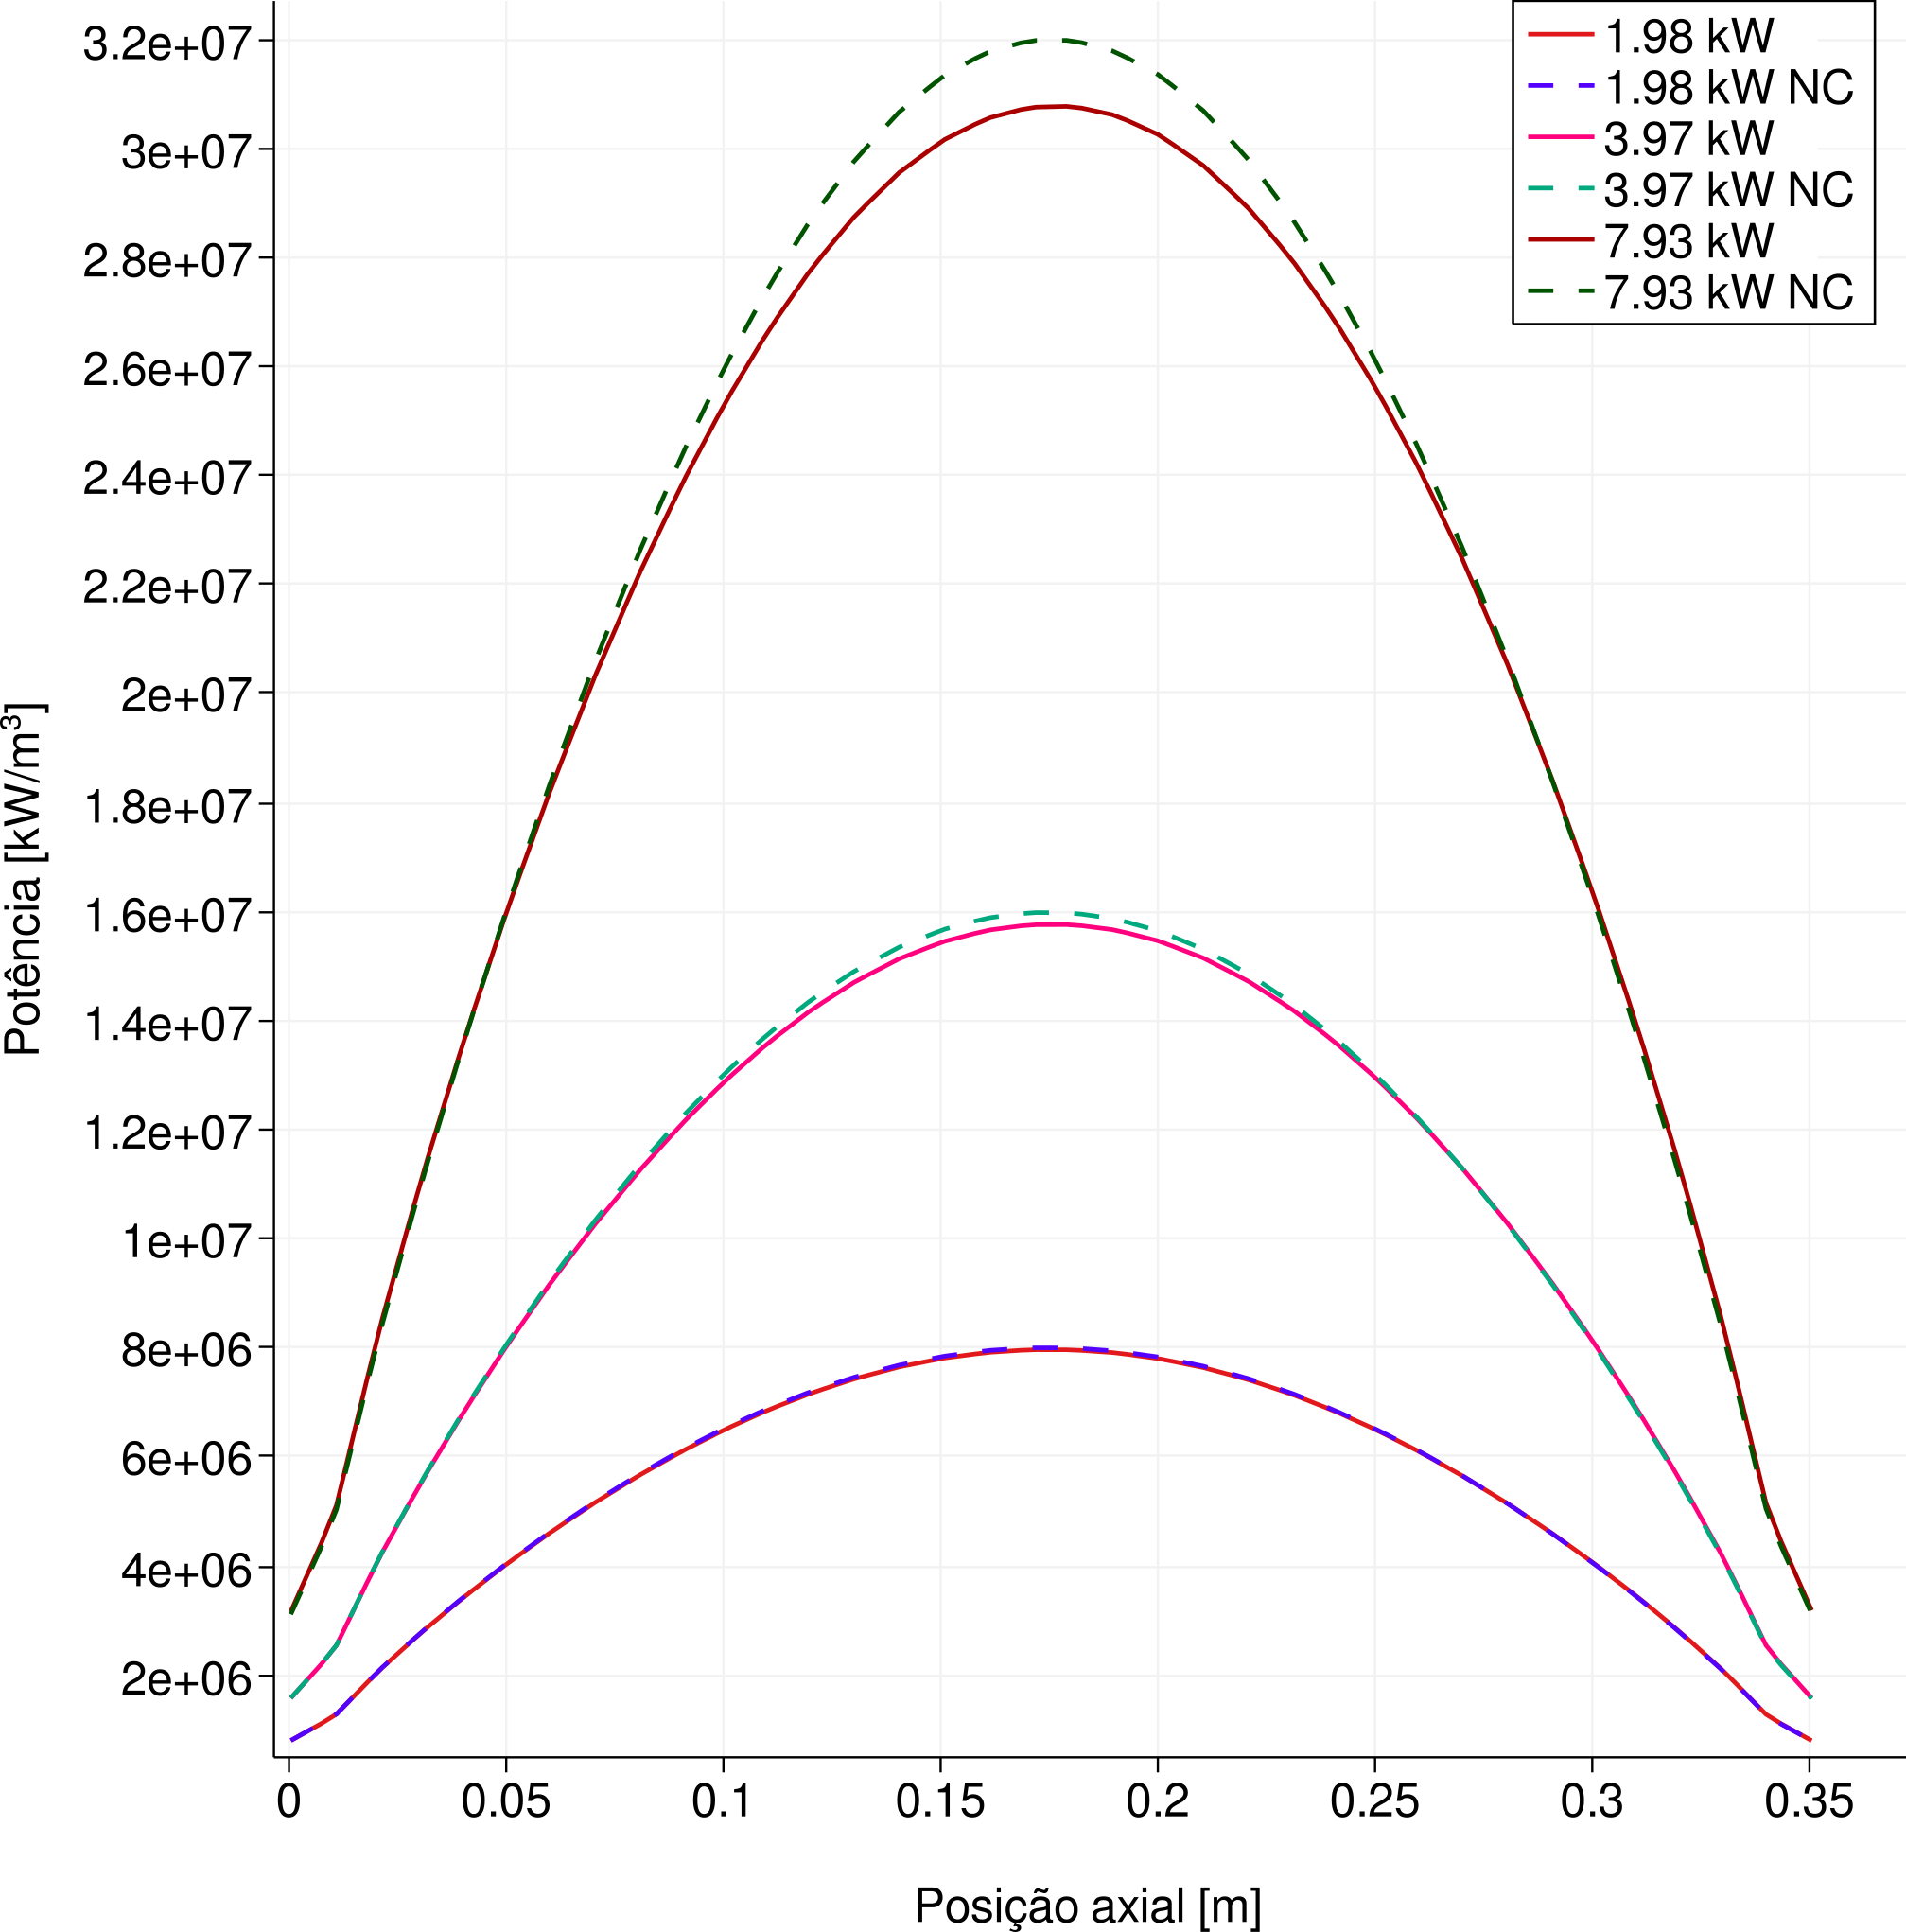
\includegraphics[width=\textwidth, height=7.0cm]{../figuras/Q_all_z_square_port.png}
  \label{fig:keff50}
\end{frame}

%-------------------------------------------------
%\subsection{Gráficos}
\begin{frame}
  \frametitle{Resultados}
  \framesubtitle{Potência: distribuição radial}
%  Distribuição de potência [$KW/m^3$].
  \centering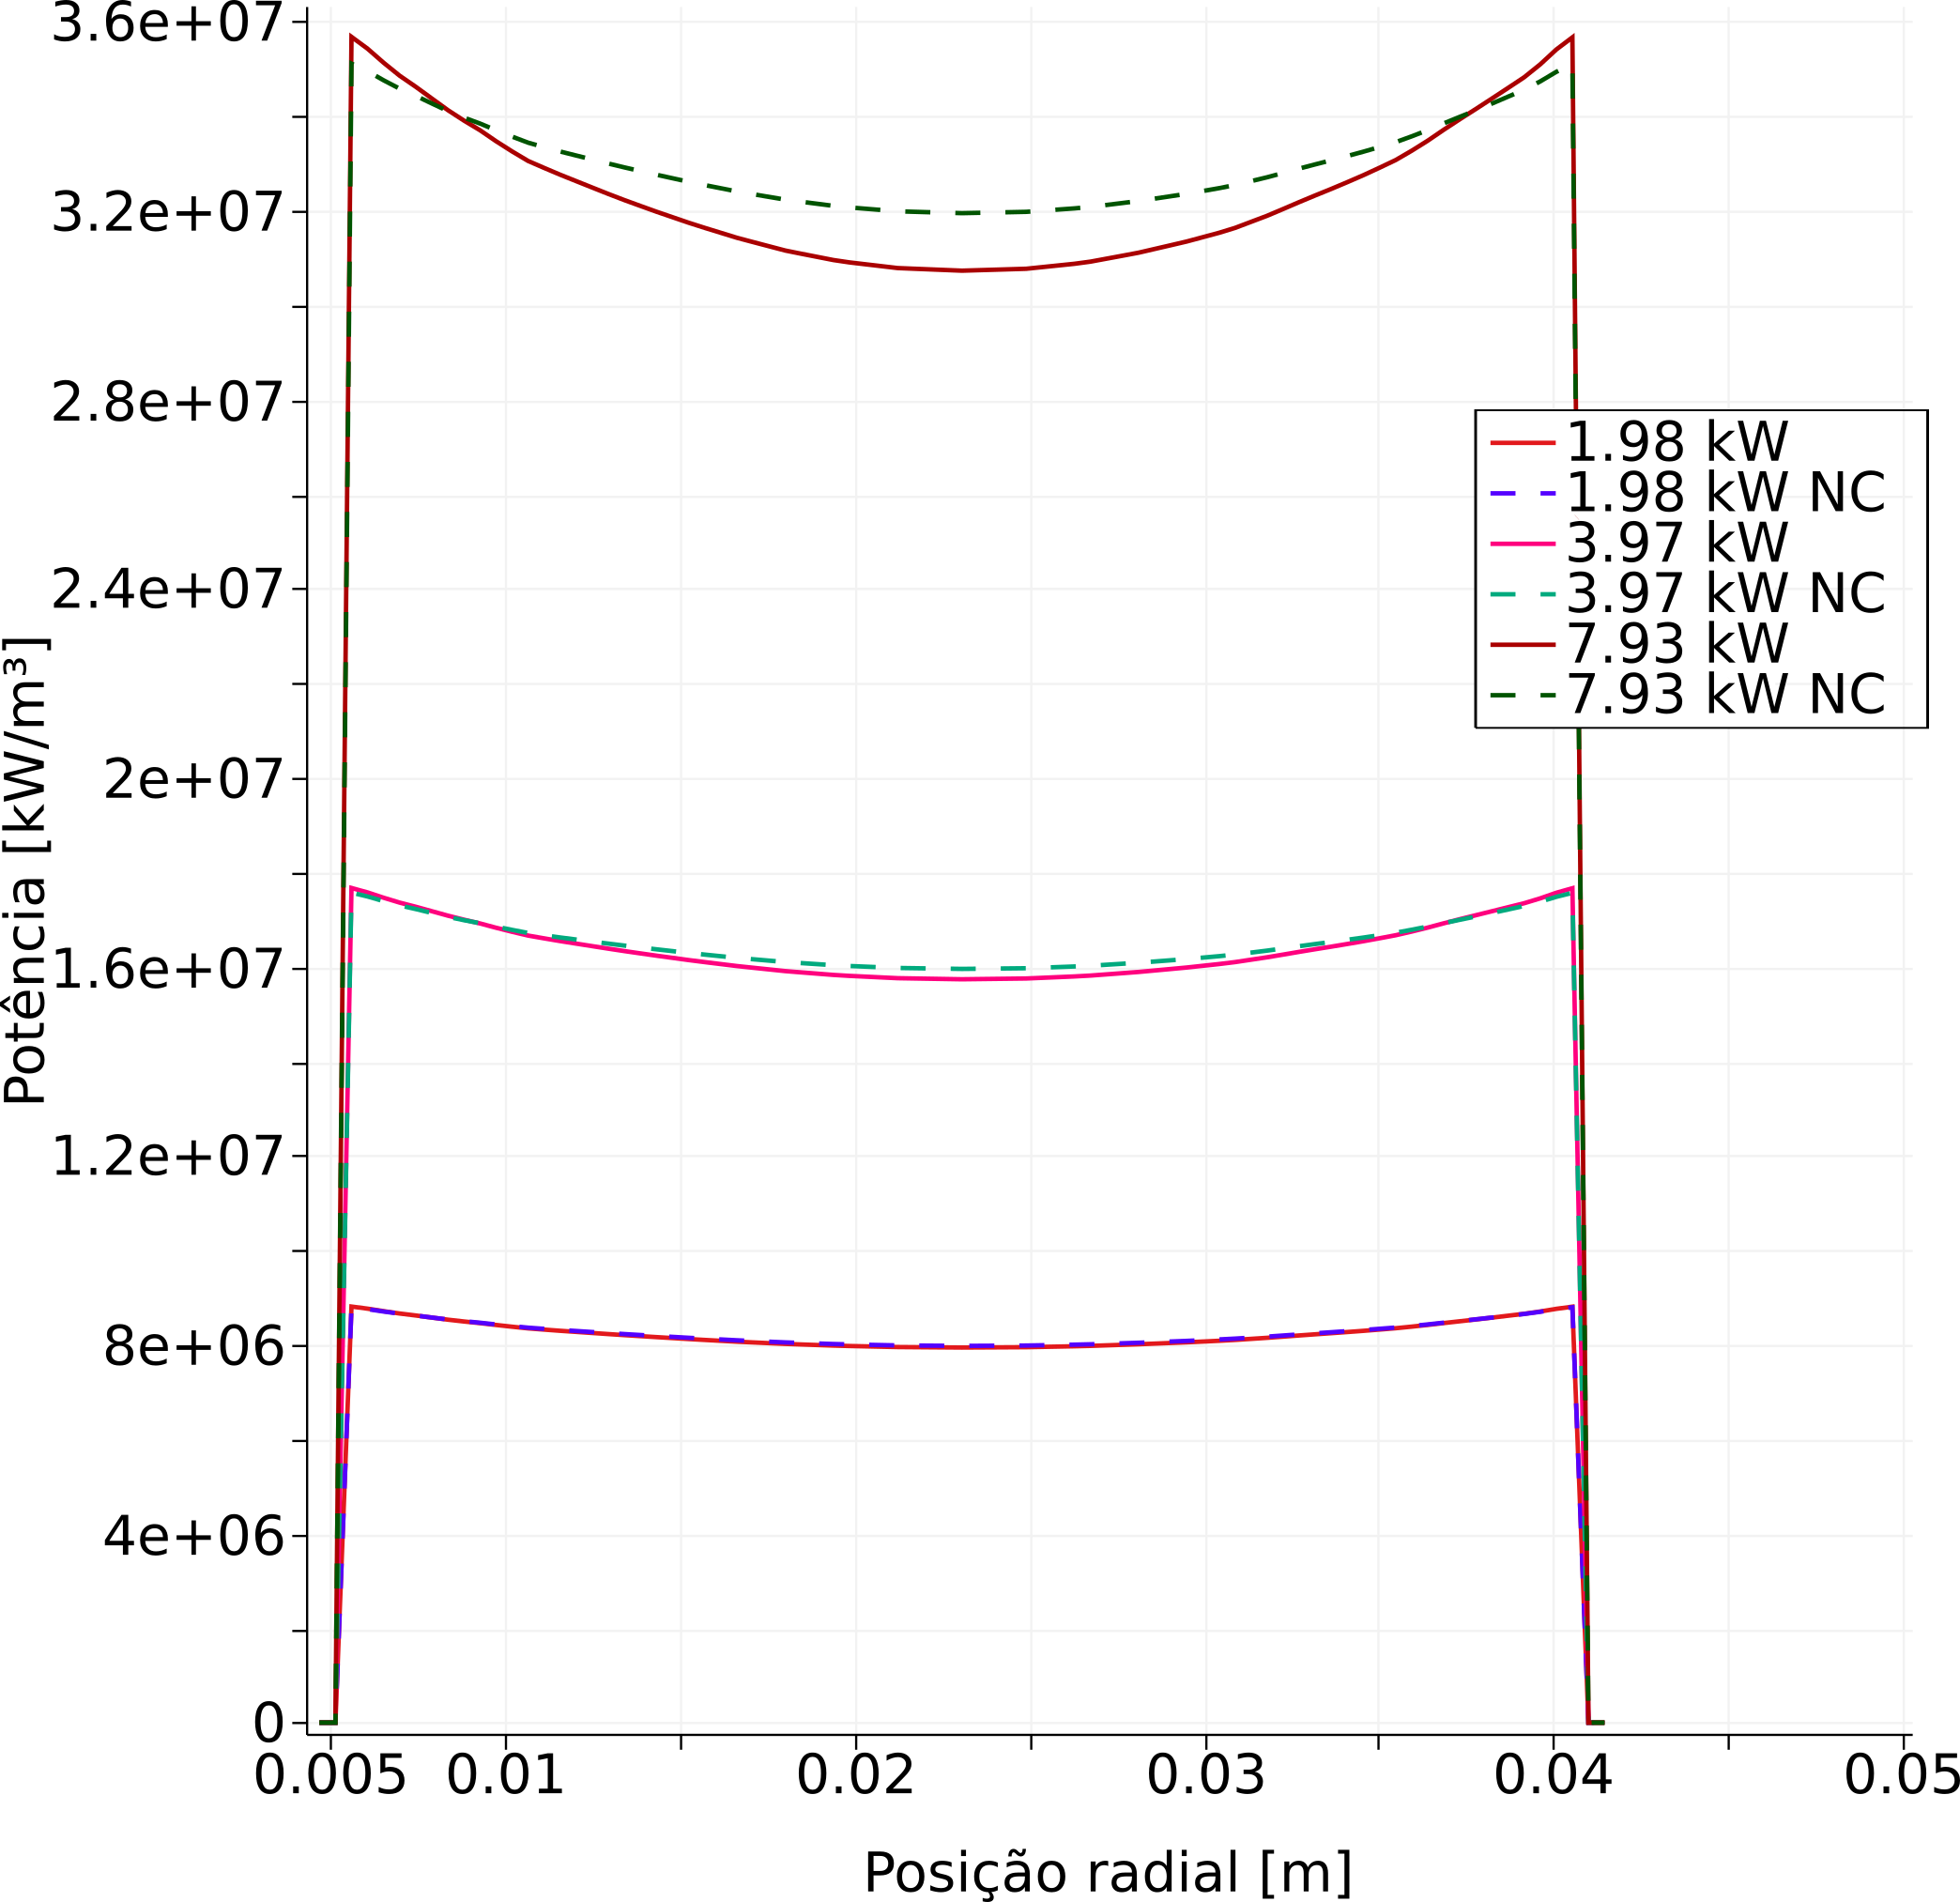
\includegraphics[width=\textwidth, height=7.0cm]{../figuras/Q_all_x_square_port.png}
  \label{fig:keff50}
\end{frame}

%-------------------------------------------------
%\subsection{Gráficos}
\begin{frame}
  \frametitle{Resultados}
  \framesubtitle{Temperatura: distribuição axial}
%  Distribuição de temperaturas [$K$].
  \centering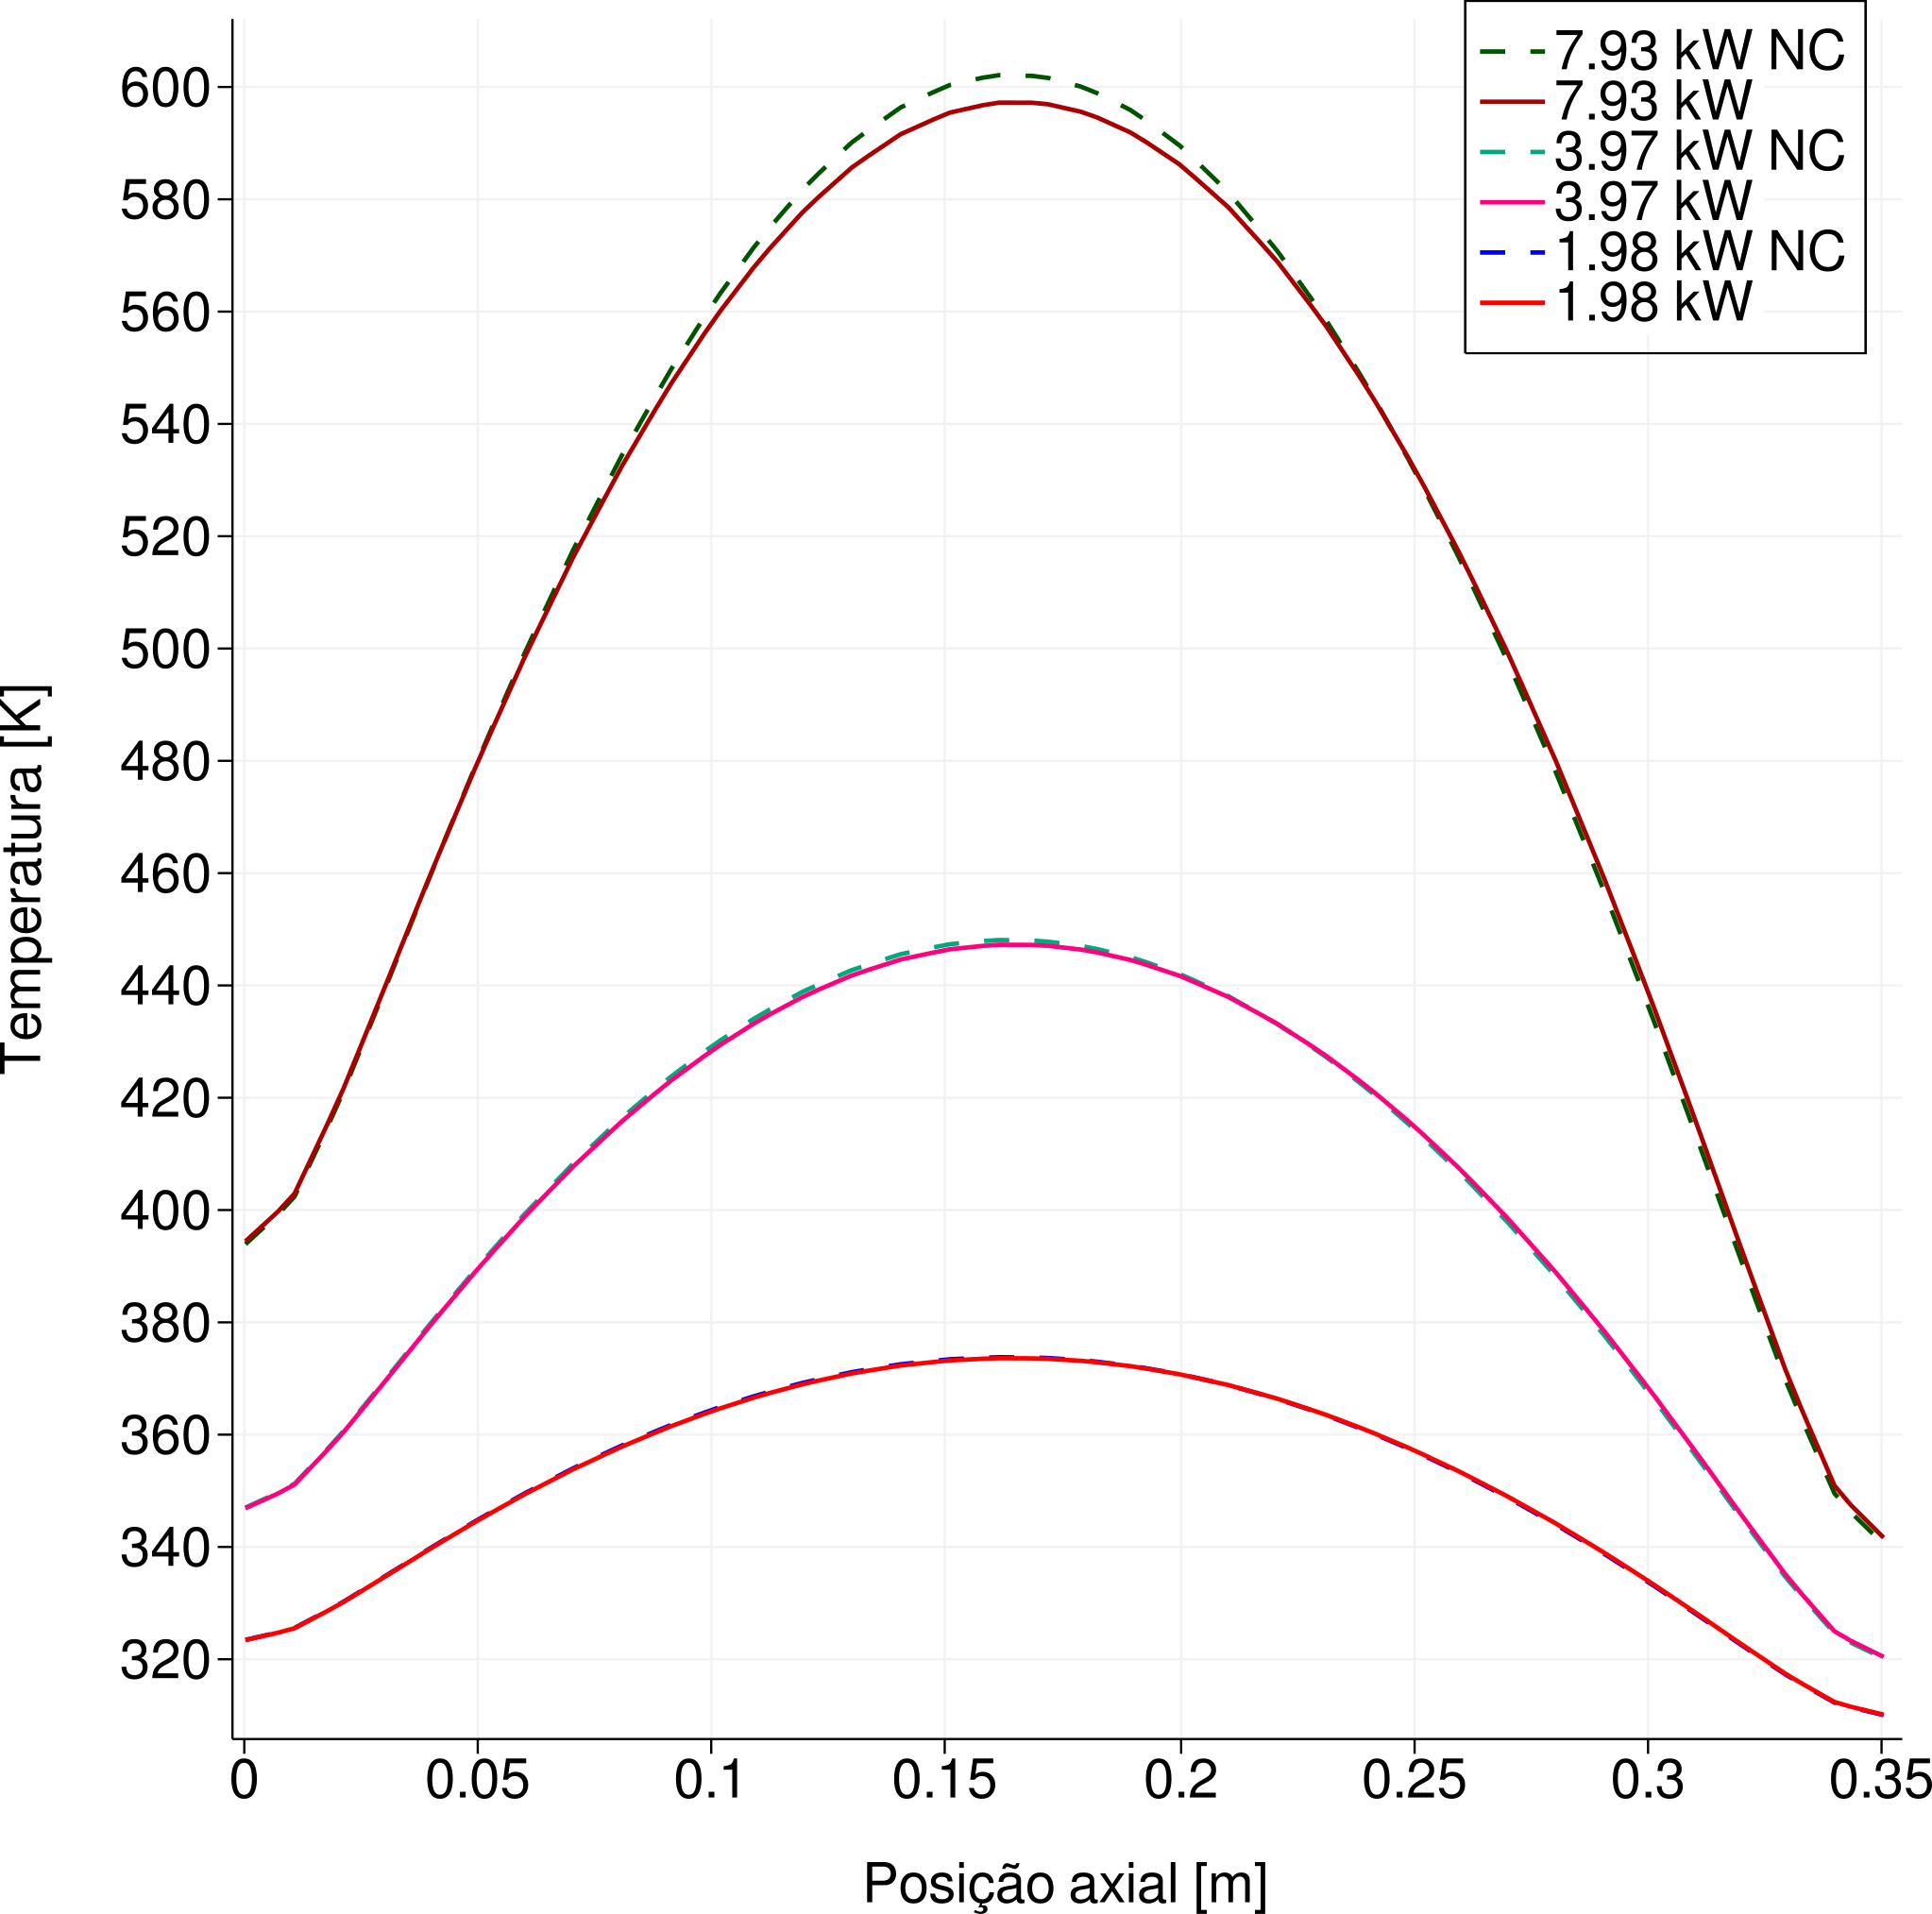
\includegraphics[width=\textwidth, height=7.0cm]{../figuras/T_z_all_square_port.png}
  \label{fig:keff50}
\end{frame}

%-------------------------------------------------
%\subsection{Gráficos}
\begin{frame}
  \frametitle{Resultados}
  \framesubtitle{Temperatura: distribuição radial}
%  Distribuição de temperaturas [$K$].
  \centering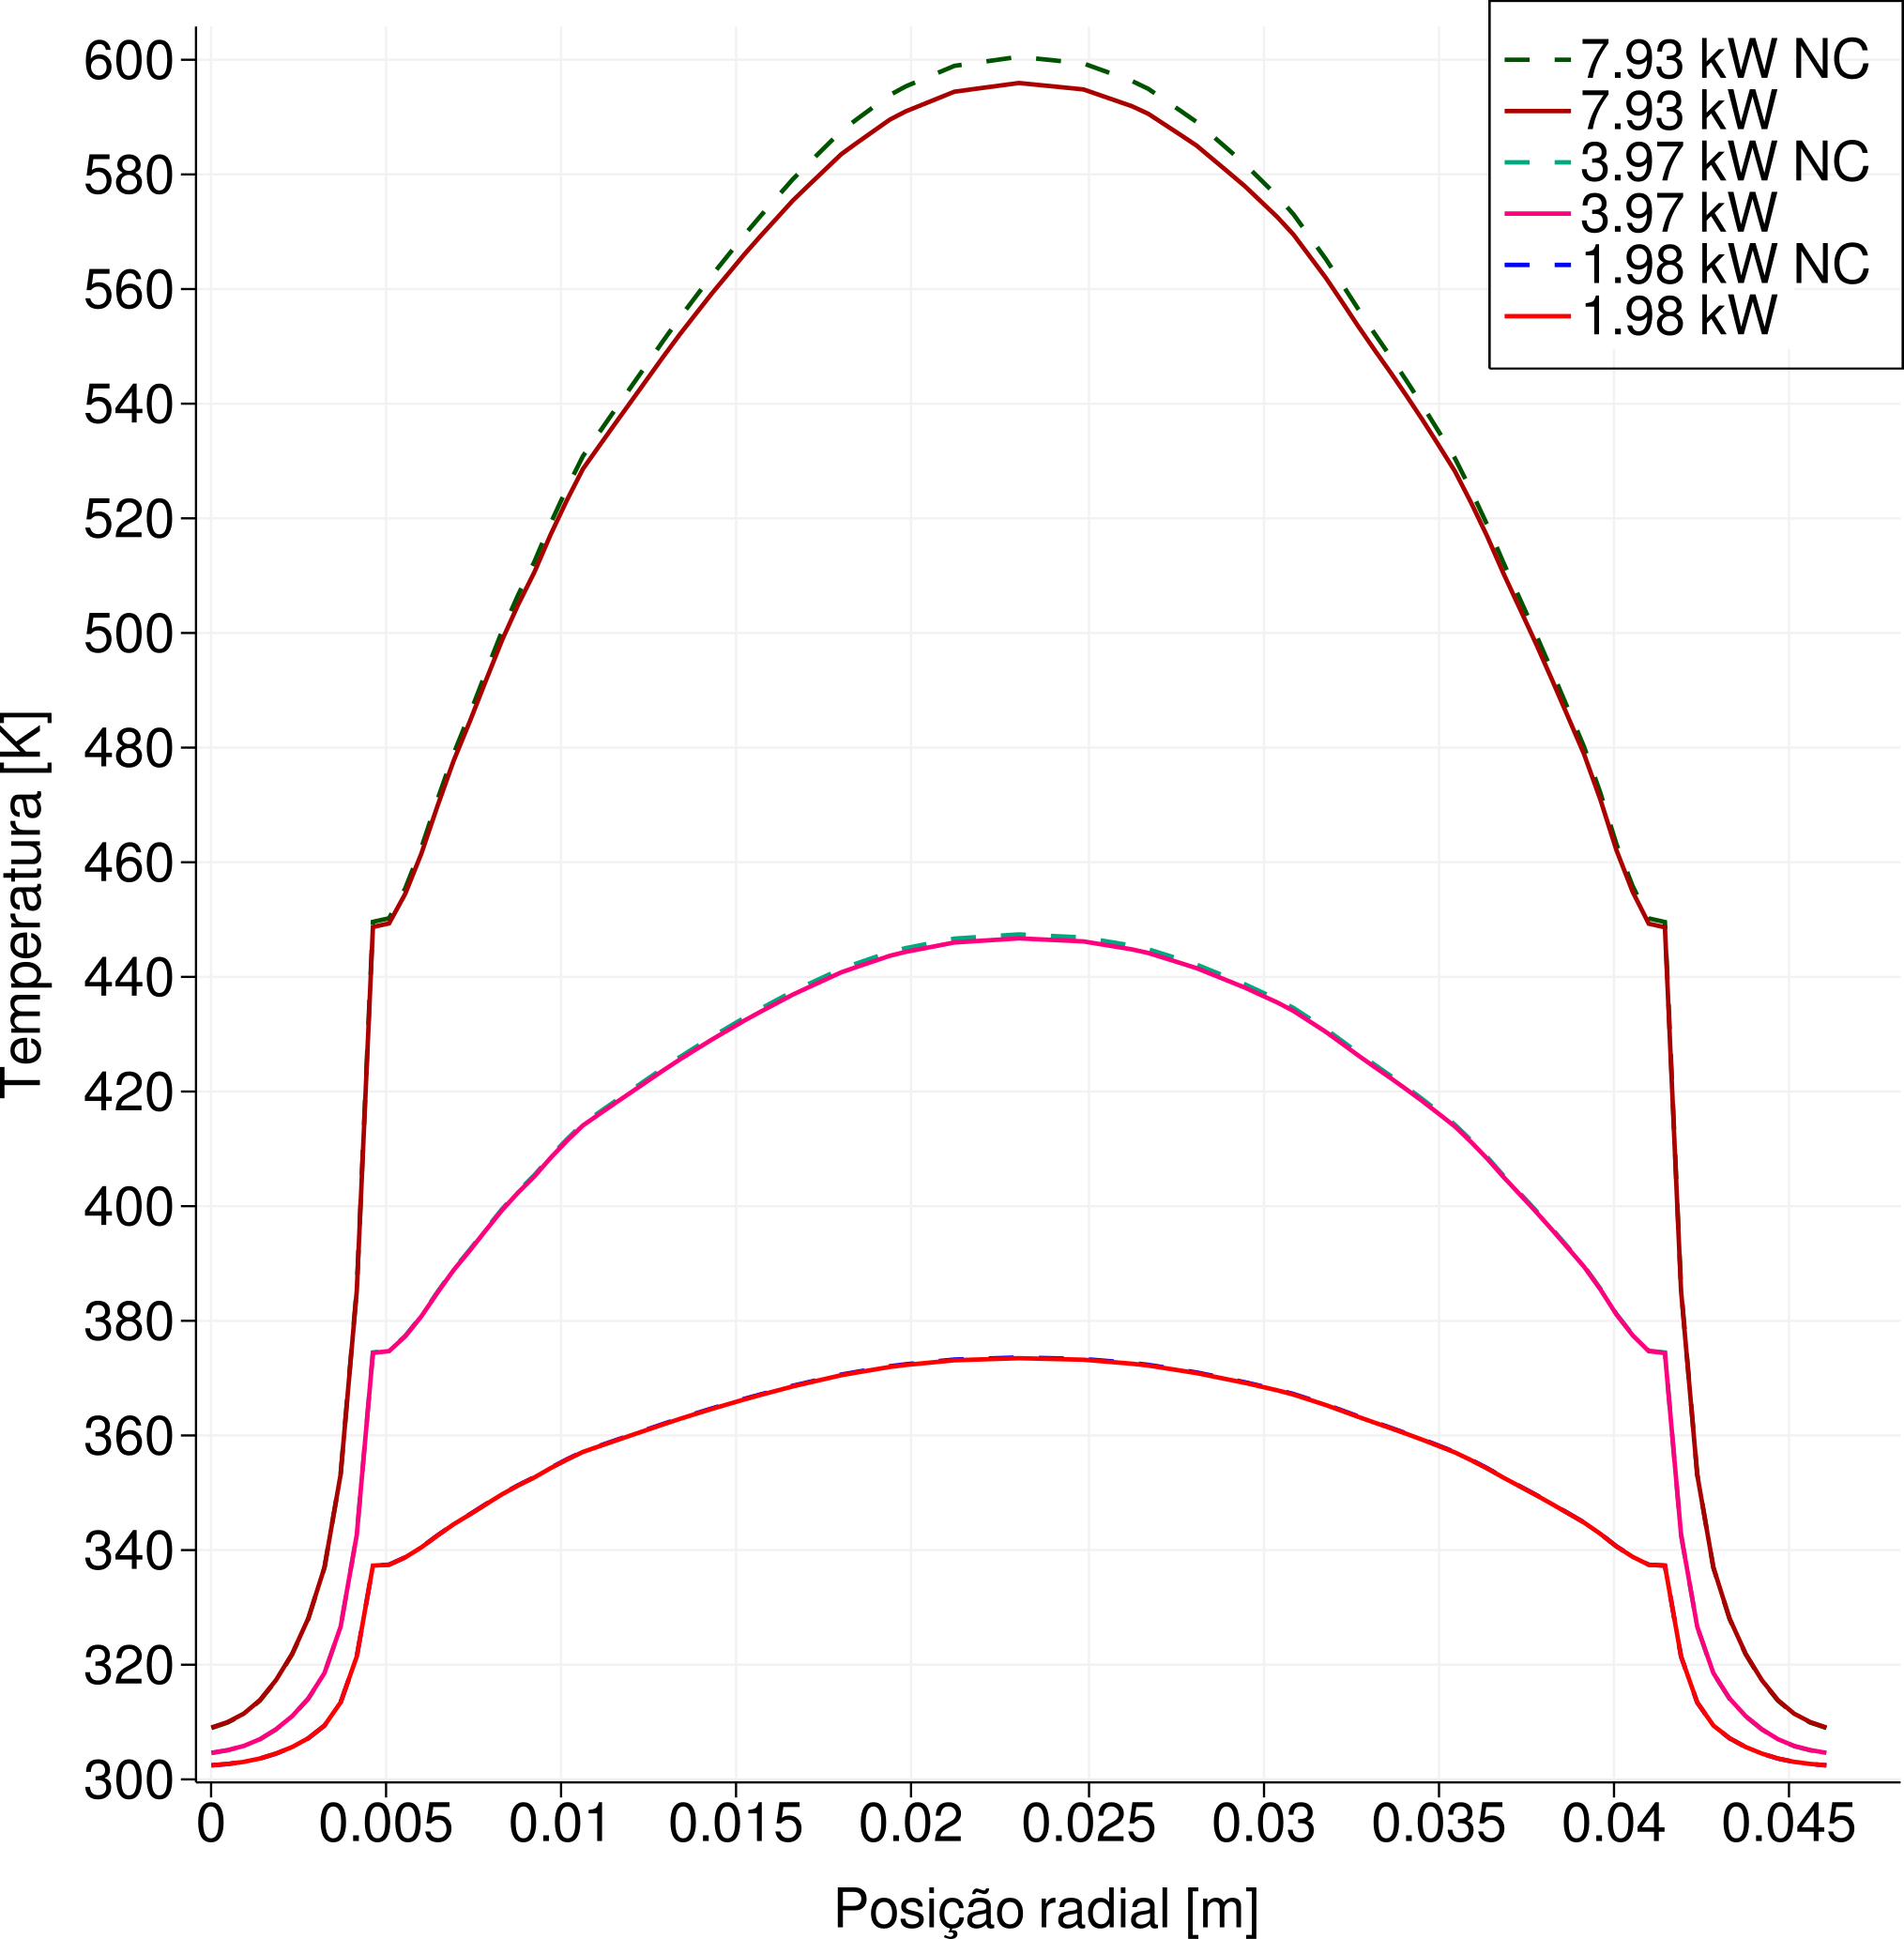
\includegraphics[width=\textwidth, height=7.0cm]{../figuras/T_x_all_square_port.png}
  \label{fig:keff50}
\end{frame}

%-------------------------------------------------
%\subsection{Gráficos}
\begin{frame}
  \frametitle{Resultados}
  \framesubtitle{Convergência}
  Variação dos fatores de multiplicação efetivo ($k_{eff}$).
  \centering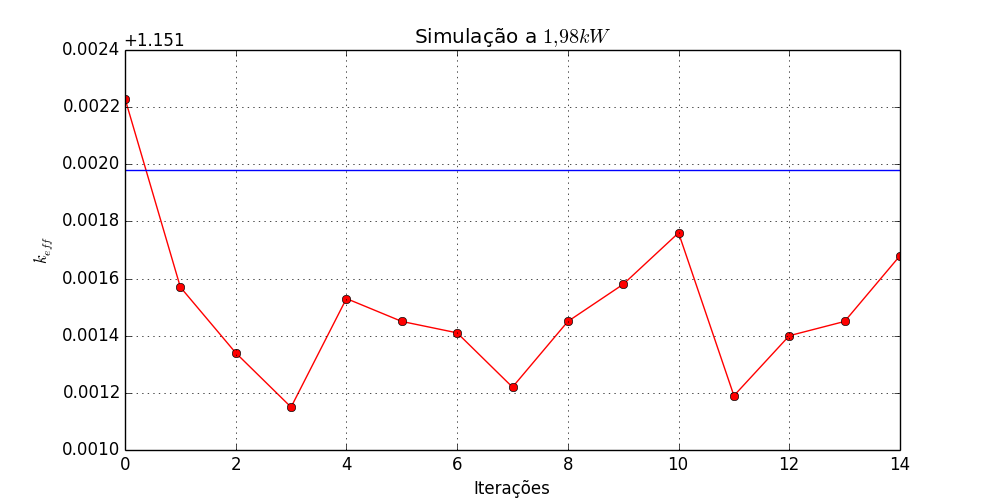
\includegraphics[scale=0.45]{../figuras/plot50.png}
  \label{fig:keff50}
\end{frame}

%-------------------------------------------------
\begin{frame}
  \frametitle{Resultados}
  \framesubtitle{Convergência}
  Variação dos fatores de multiplicação efetivo ($k_{eff}$).
  \centering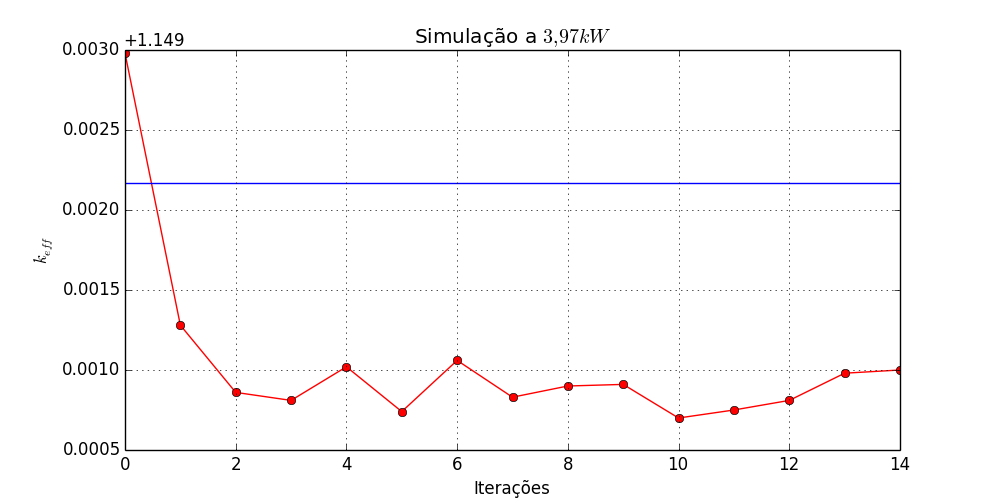
\includegraphics[scale=0.45]{../figuras/plot100.png}
  \label{fig:keff100}
\end{frame}

%-------------------------------------------------
\begin{frame}
  \frametitle{Resultados}
  \framesubtitle{Convergência}
  Variação dos fatores de multiplicação efetivo ($k_{eff}$).
  \centering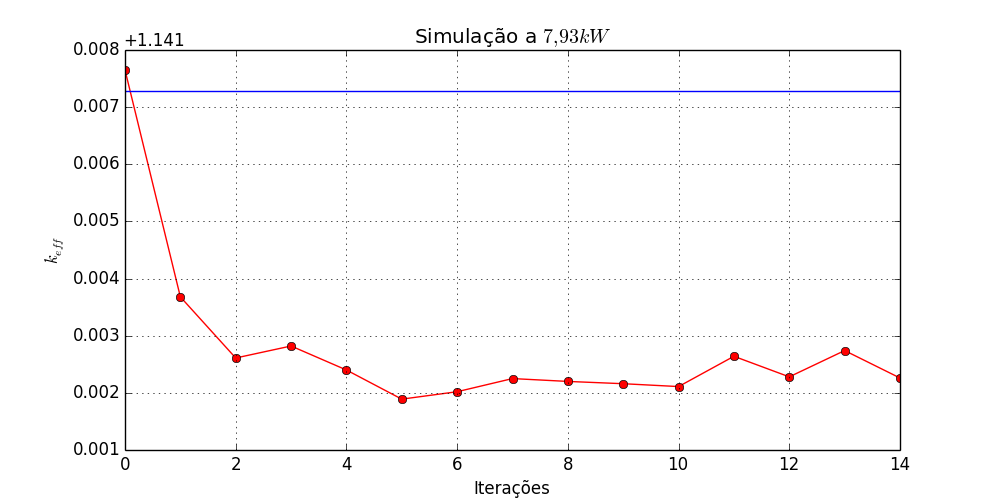
\includegraphics[scale=0.45]{../figuras/plot200.png}
  \label{fig:keff200}
\end{frame}




%-------------------------------------------------
\subsection{Fator de multiplicação}
\begin{frame}
  \frametitle{Resultados}
  \framesubtitle{Fator de multiplicação}
\begin{table}[]
\centering
%\caption{My caption}
\begin{tabular}{l|r|r|r|}
\cline{2-4}
\multicolumn{1}{c|}{}          & \multicolumn{3}{c|}{$k_{eff}$}                                                                                                                                              \\ \hline
\multicolumn{1}{|c|}{Potência} & \multicolumn{1}{c|}{Não acoplado} & \multicolumn{1}{c|}{\begin{tabular}[c]{@{}c@{}}Acoplado\\ (média durante \\os cálculos)\end{tabular}} & \multicolumn{1}{c|}{Desvio padrão} \\ \hline
\multicolumn{1}{|l|}{1,98 kW}  & 1,15298                           & 1,15249                                                                                             & 0,000257                           \\ \hline
\multicolumn{1}{|l|}{3,97 kW}  & 1,15117                           & 1,15004                                                                                             & 0,000538                           \\ \hline
\multicolumn{1}{|l|}{7,93 kW}  & 1,14829                           & 1,14378                                                                                             & 0,001367                           \\ \hline
\end{tabular}
\end{table}
\end{frame}

%-------------------------------------------------
\begin{frame}
  \frametitle{Resultados}
  \framesubtitle{Robustez(?)}
  Variação do fator de multiplicação efetivo ($k_{eff}$) com mudanças em parâmetros de convergência.
  \centering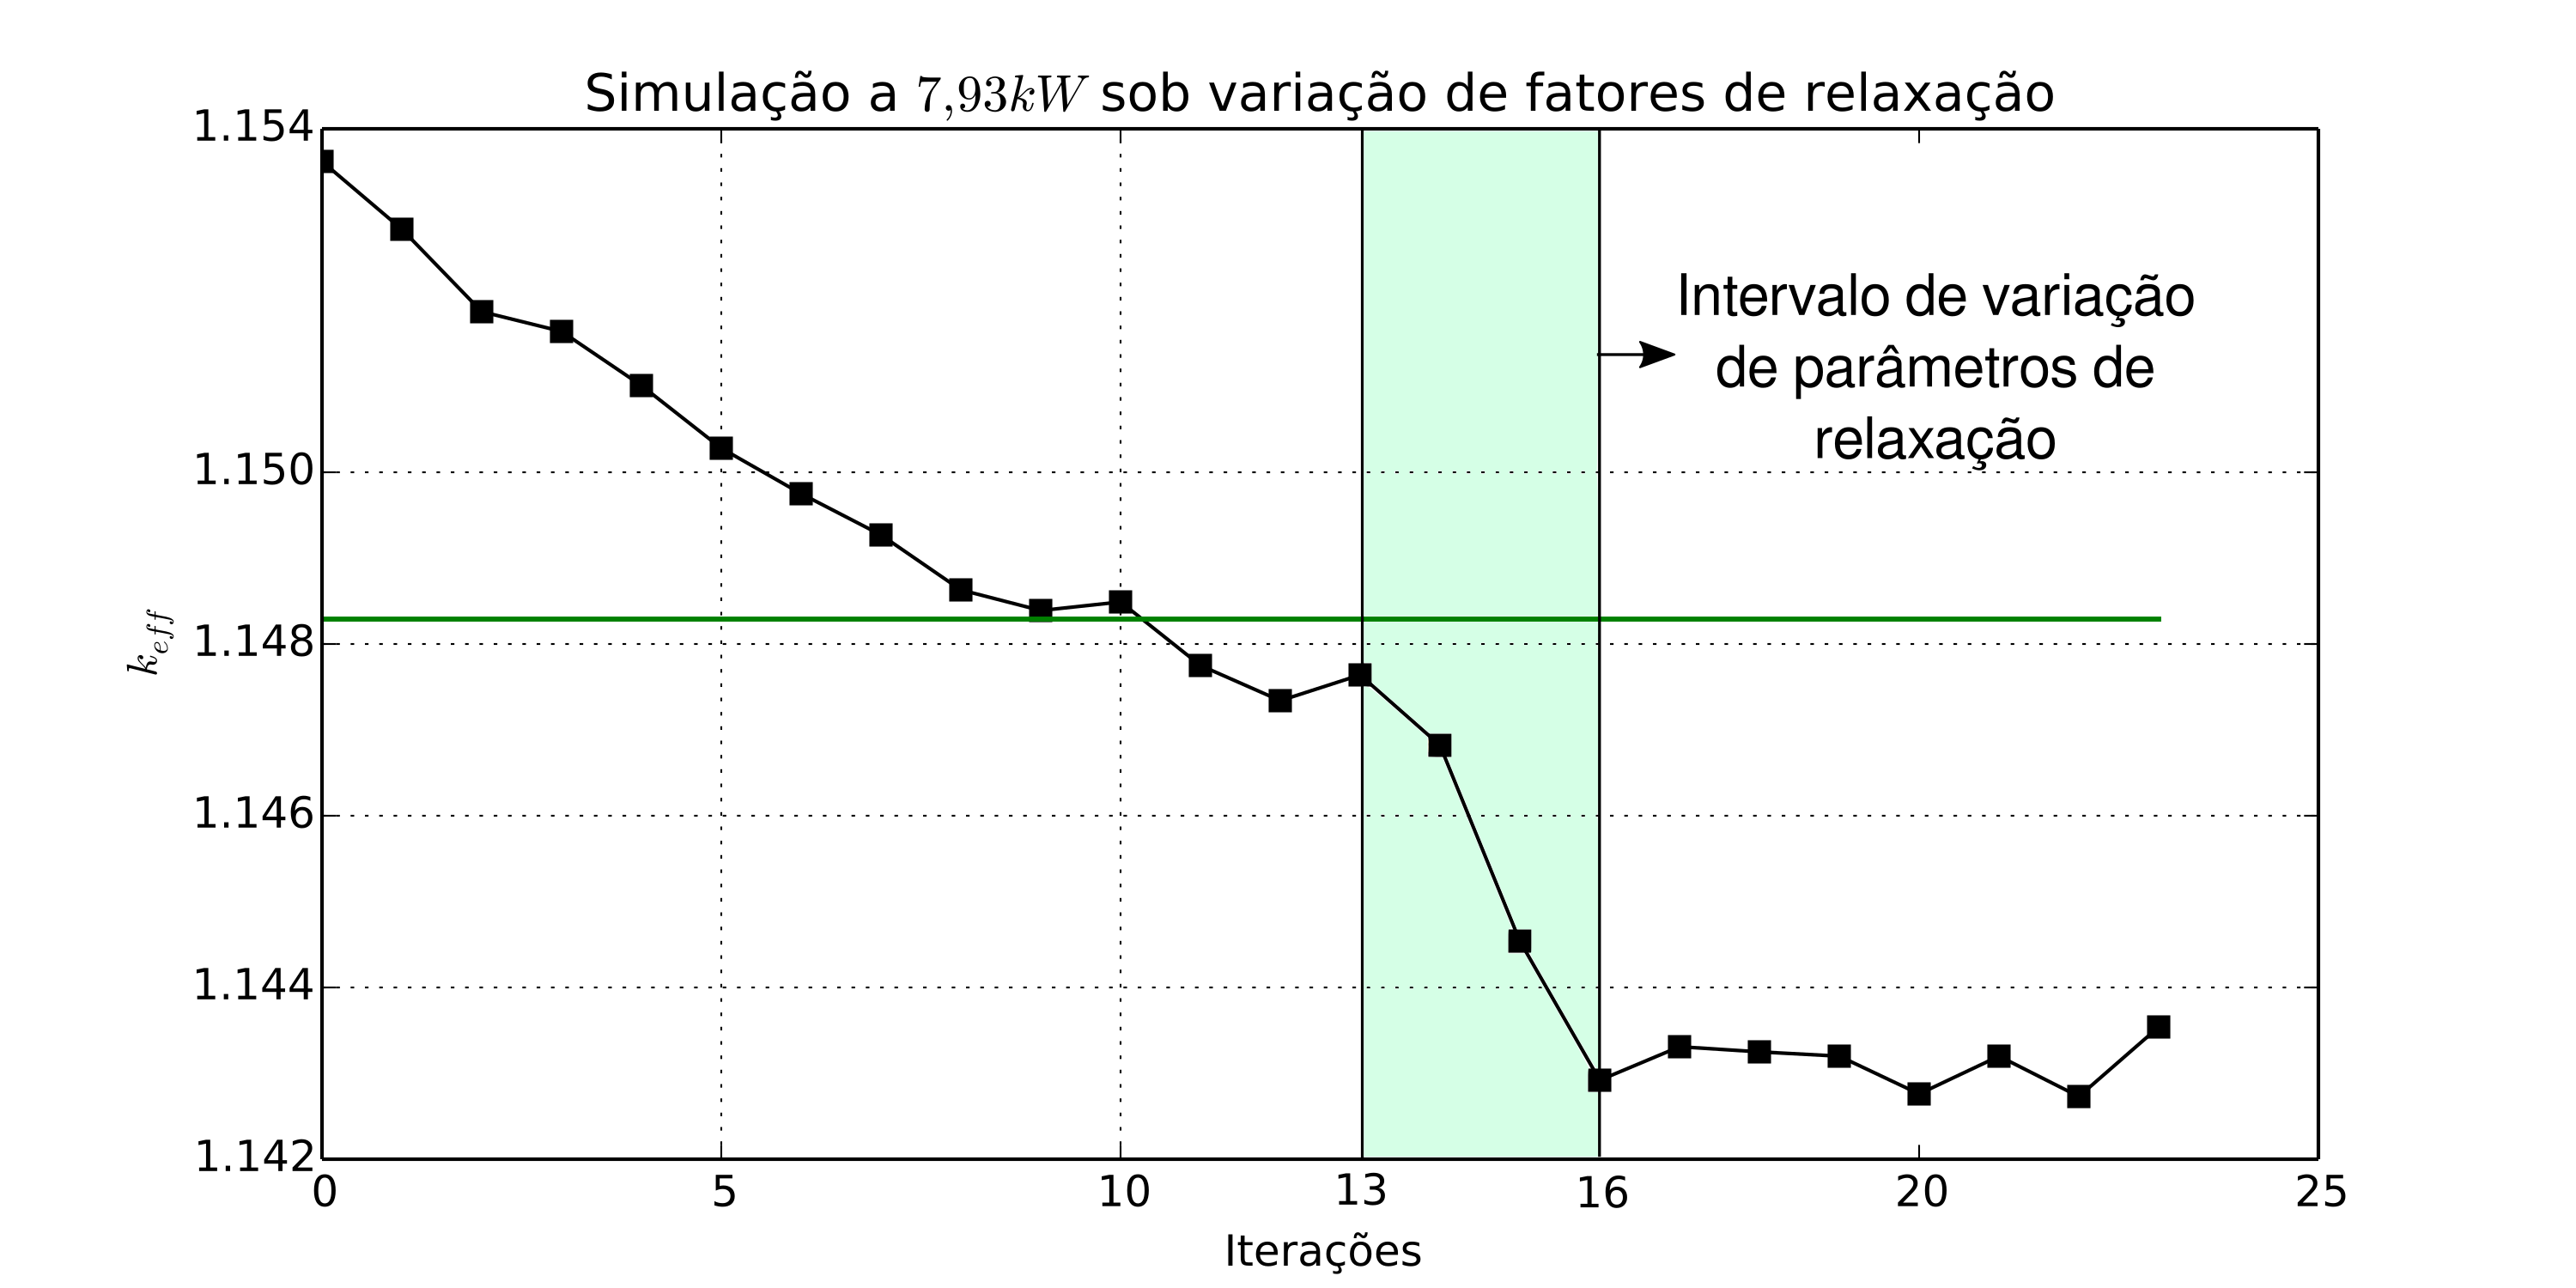
\includegraphics[scale=0.45]{../figuras/plot200-disturb-port.png}
  \label{fig:keff_dist}
%  \legend{Fonte: autor}
\end{frame}

\section{Conclusões}
%-------------------------------------------------
\begin{frame}
  \frametitle{Conclusões}
  \framesubtitle{}
  \begin{itemize}
  \item Desenvolvido um sistema livre, aberto e gratuito para cálculos neutrônicos e termo-hidráulicos acoplados utilizado a mesma malha;
  \item Desenvolvida uma metodologia para a construção do sistema acoplado baseado em sistemas já existentes e utilizando memória compartilhada
    para intercâmbio de dados;
  \item O sistema desenvolvido é inovador nas suas caracteríticas;
  \end{itemize}
\end{frame}

%-------------------------------------------------
\begin{frame}
  \frametitle{Conclusões}
  \framesubtitle{}
  \begin{columns}
    \column{0.5\textwidth}
    Vantagens:
    \column{0.5\textwidth}
    Desvantagens:
  \end{columns}
\end{frame}

%-------------------------------------------------
\begin{frame}
  \frametitle{Conclusões}
  \framesubtitle{Discussão sobre \textit{software} livre}
\end{frame}

%-------------------------------------------------
\begin{frame}
  \frametitle{Conclusões}
  \framesubtitle{Trabalhos futuros}
\end{frame}



%-------------------------------------------------
\begin{frame}[allowframebreaks]
        \frametitle{Referências}
        \bibliographystyle{amsalpha}
        \bibliography{apre.bib}
\end{frame}


%-------------------------------------------------
% Frame escondido
\begin{frame}[noframenumbering]
  \frametitle{Respostas}
  \framesubtitle{Seções de choque}
  Teste
\end{frame}


\end{document}

